\documentclass[12pt,a4paper]{article}

% ============================================================================
% C++ / Технологии программирования — общая преамбула конспекта
% Движок: XeLaTeX
% Основной стандарт примеров: C++17, если явно не указано иное.
% ============================================================================

% ---------- Язык, Unicode и шрифты ------------------------------------------
\usepackage{fontspec}
\usepackage{polyglossia}
\setdefaultlanguage{russian}
\setotherlanguage{english}

\defaultfontfeatures{Ligatures=TeX,Scale=MatchLowercase}
\setmainfont{DejaVu Serif}
\setsansfont{DejaVu Sans}
\setmonofont{DejaVu Sans Mono}

% ---------- Геометрия и базовая типографика --------------------------------
\usepackage[a4paper,top=20mm,bottom=22mm,left=22mm,right=18mm,headheight=15pt]{geometry}
\usepackage{microtype}
\usepackage{setspace}
\usepackage{parskip}
\usepackage{ragged2e}
\usepackage{enumitem}
\usepackage{titlesec}

\setlength{\parindent}{0pt}
\setlength{\parskip}{0.55em}
\setlist{nosep,leftmargin=2em}
\emergencystretch=2em

% ---------- Математика -------------------------------------------------------
\usepackage{amsmath}
\usepackage{amssymb}
\usepackage{mathtools}
\usepackage{amsthm}

% ---------- Цвета ------------------------------------------------------------
\usepackage{xcolor}

\definecolor{CppBlue}{HTML}{1F4E79}
\definecolor{CppDark}{HTML}{202124}
\definecolor{CppGray}{HTML}{5F6368}
\definecolor{CppLightGray}{HTML}{F4F5F7}
\definecolor{CppBorder}{HTML}{D0D7DE}
\definecolor{CppGreen}{HTML}{2E7D32}
\definecolor{CppOrange}{HTML}{B35C00}
\definecolor{CppRed}{HTML}{B42318}
\definecolor{CppPurple}{HTML}{6F42C1}
\definecolor{CppCyan}{HTML}{006D77}
\definecolor{CppYellowBg}{HTML}{FFF8DC}
\definecolor{CppRedBg}{HTML}{FFF1F0}
\definecolor{CppGreenBg}{HTML}{F1F8F3}
\definecolor{CppBlueBg}{HTML}{EEF6FF}
\definecolor{CppPurpleBg}{HTML}{F7F2FF}

% ---------- Рисунки, таблицы, плавающие объекты -----------------------------
\usepackage{graphicx}
\usepackage{eso-pic}
\usepackage{float}
\usepackage{booktabs}
\usepackage{tabularx}
\usepackage{longtable}
\usepackage{array}
\usepackage{multirow}
\usepackage{caption}
\usepackage{subcaption}

\graphicspath{{./}{figures/}{images/}}
\captionsetup{font=small,labelfont=bf}

\newcolumntype{Y}{>{\RaggedRight\arraybackslash}X}
\newcolumntype{C}[1]{>{\centering\arraybackslash}p{#1}}
\newcolumntype{L}[1]{>{\RaggedRight\arraybackslash}p{#1}}

% ---------- Ссылки -----------------------------------------------------------
\usepackage{hyperref}
\usepackage{xurl}
\usepackage[nameinlink,noabbrev]{cleveref}

\hypersetup{
  unicode=true,
  colorlinks=true,
  linkcolor=CppBlue,
  citecolor=CppGreen,
  urlcolor=CppPurple,
  pdfborder={0 0 0}
}

\urlstyle{same}

% ---------- Колонтитулы ------------------------------------------------------
\usepackage{fancyhdr}
\pagestyle{fancy}
\fancyhf{}
\fancyhead[L]{\small\sffamily Технологии программирования и C++}
\fancyhead[R]{\small\sffamily\nouppercase{\leftmark}}
\fancyfoot[C]{\small\sffamily\thepage}
\renewcommand{\headrulewidth}{0.4pt}
\renewcommand{\footrulewidth}{0pt}

% ---------- Код: listings ----------------------------------------------------
% listings выбран намеренно без shell-escape: PDF должен собираться обычным
% XeLaTeX. Основной код примеров — ASCII; русские пояснения даются вне листинга.
\usepackage{listings}
\usepackage{upquote}

\lstdefinestyle{codebase}{
  basicstyle=\ttfamily\small,
  backgroundcolor=\color{CppLightGray},
  frame=single,
  rulecolor=\color{CppBorder},
  framerule=0.5pt,
  framesep=7pt,
  xleftmargin=0.5em,
  xrightmargin=0.5em,
  breaklines=true,
  breakatwhitespace=false,
  postbreak=\mbox{\textcolor{CppGray}{$\hookrightarrow$}\space},
  columns=fullflexible,
  keepspaces=true,
  showstringspaces=false,
  showtabs=false,
  tabsize=4,
  captionpos=b,
  aboveskip=0.9em,
  belowskip=0.9em,
  escapeinside={(*@}{@*)},
  literate={~}{{\textasciitilde}}1
           {^}{{\textasciicircum}}1
}

\lstdefinestyle{cpp}{
  style=codebase,
  language=C++,
  keywordstyle=\bfseries\color{CppBlue},
  keywordstyle=[2]\bfseries\color{CppPurple},
  commentstyle=\itshape\color{CppGreen},
  stringstyle=\color{CppOrange},
  numberstyle=\scriptsize\color{CppGray},
  numbers=left,
  numbersep=9pt,
  morekeywords=[2]{override,final,noexcept,nullptr,constexpr,decltype,alignas,alignof,
                   static_assert,thread_local,concept,requires,co_await,co_yield,co_return}
}

\lstdefinestyle{cppplain}{
  style=cpp,
  numbers=none
}

\lstdefinestyle{shell}{
  style=codebase,
  language=bash,
  numbers=none,
  keywordstyle=\bfseries\color{CppBlue},
  commentstyle=\itshape\color{CppGreen},
  stringstyle=\color{CppOrange}
}

\lstdefinelanguage{CMake}{
  sensitive=false,
  morekeywords={cmake_minimum_required,project,add_executable,add_library,
    target_compile_features,target_compile_options,target_include_directories,
    target_link_libraries,set,option,if,elseif,else,endif,foreach,endforeach,
    function,endfunction,include,find_package,enable_testing,add_test,
    install,FetchContent_Declare,FetchContent_MakeAvailable},
  morecomment=[l]{\#},
  morestring=[b]"
}

\lstdefinestyle{cmake}{
  style=codebase,
  language=CMake,
  numbers=left,
  numberstyle=\scriptsize\color{CppGray},
  numbersep=9pt,
  keywordstyle=\bfseries\color{CppPurple},
  commentstyle=\itshape\color{CppGreen},
  stringstyle=\color{CppOrange}
}

\lstdefinelanguage{Diff}{
  morecomment=[f][\color{CppGreen}]{+},
  morecomment=[f][\color{CppRed}]{-},
  morecomment=[f][\color{CppCyan}]{@@}
}

\lstdefinestyle{diff}{
  style=codebase,
  language=Diff,
  numbers=none
}

\lstdefinestyle{output}{
  style=codebase,
  numbers=none,
  basicstyle=\ttfamily\footnotesize,
  backgroundcolor=\color{white},
  rulecolor=\color{CppBorder}
}

% Основные окружения для вставки кода.
\lstnewenvironment{cppcode}[1][]
  {\lstset{style=cpp,#1}}
  {}

\lstnewenvironment{cppcodeplain}[1][]
  {\lstset{style=cppplain,#1}}
  {}

\lstnewenvironment{shellcode}[1][]
  {\lstset{style=shell,#1}}
  {}

\lstnewenvironment{cmakecode}[1][]
  {\lstset{style=cmake,#1}}
  {}

\lstnewenvironment{outputcode}[1][]
  {\lstset{style=output,#1}}
  {}

\lstnewenvironment{diffcode}[1][]
  {\lstset{style=diff,#1}}
  {}

% Короткий inline-код. Использование: \cppinline|std::vector<int>|
\newcommand{\cppinline}{\lstinline[style=cppplain]}
\newcommand{\shellinline}{\lstinline[style=shell]}

% ---------- Цветные смысловые блоки -----------------------------------------
\usepackage[most]{tcolorbox}
\tcbuselibrary{breakable,skins,theorems,listings}

\newtcolorbox{importantbox}[1][Важно]{
  enhanced,breakable,
  colback=CppBlueBg,colframe=CppBlue,
  boxrule=0.7pt,arc=1.5mm,
  title={#1},fonttitle=\bfseries,
  left=1.2mm,right=1.2mm,top=1mm,bottom=1mm
}

\newtcolorbox{warningbox}[1][Осторожно]{
  enhanced,breakable,
  colback=CppYellowBg,colframe=CppOrange,
  boxrule=0.7pt,arc=1.5mm,
  title={#1},fonttitle=\bfseries,
  left=1.2mm,right=1.2mm,top=1mm,bottom=1mm
}

\newtcolorbox{ubbox}[1][Undefined behavior]{
  enhanced,breakable,
  colback=CppRedBg,colframe=CppRed,
  boxrule=0.8pt,arc=1.5mm,
  title={#1},fonttitle=\bfseries,
  left=1.2mm,right=1.2mm,top=1mm,bottom=1mm
}

\newtcolorbox{practicebox}[1][Практика]{
  enhanced,breakable,
  colback=CppGreenBg,colframe=CppGreen,
  boxrule=0.7pt,arc=1.5mm,
  title={#1},fonttitle=\bfseries,
  left=1.2mm,right=1.2mm,top=1mm,bottom=1mm
}

\newtcolorbox{performancebox}[1][Производительность]{
  enhanced,breakable,
  colback=CppPurpleBg,colframe=CppPurple,
  boxrule=0.7pt,arc=1.5mm,
  title={#1},fonttitle=\bfseries,
  left=1.2mm,right=1.2mm,top=1mm,bottom=1mm
}

\newtcolorbox{implementationbox}[1][Типичная реализация]{
  enhanced,breakable,
  colback=CppLightGray,colframe=CppGray,
  boxrule=0.7pt,arc=1.5mm,
  title={#1},fonttitle=\bfseries,
  left=1.2mm,right=1.2mm,top=1mm,bottom=1mm
}

\newtcolorbox{standardbox}[1][Что гарантирует стандарт]{
  enhanced,breakable,
  colback=white,colframe=CppCyan,
  boxrule=0.8pt,arc=1.5mm,
  title={#1},fonttitle=\bfseries,
  left=1.2mm,right=1.2mm,top=1mm,bottom=1mm
}

\newtcolorbox{whybox}[1][Почему?]{
  enhanced,breakable,
  colback=white,colframe=CppBlue,
  borderline west={2.2pt}{0pt}{CppBlue},
  boxrule=0pt,arc=0mm,
  title={#1},fonttitle=\bfseries,
  left=2mm,right=1mm,top=1mm,bottom=1mm
}

\newtcolorbox{mistakebox}[1][Типичная ошибка]{
  enhanced,breakable,
  colback=CppRedBg,colframe=CppRed,
  borderline west={2.2pt}{0pt}{CppRed},
  boxrule=0pt,arc=0mm,
  title={#1},fonttitle=\bfseries,
  left=2mm,right=1mm,top=1mm,bottom=1mm
}

% ---------- Определения, утверждения, леммы ---------------------------------
\theoremstyle{definition}
\newtheorem{definition}{Определение}[section]
\newtheorem{example}{Пример}[section]
\newtheorem{exercise}{Упражнение}[section]

\theoremstyle{plain}
\newtheorem{theorem}{Теорема}[section]
\newtheorem{lemma}{Лемма}[section]
\newtheorem{proposition}{Утверждение}[section]
\newtheorem{corollary}{Следствие}[section]

\theoremstyle{remark}
\newtheorem{remark}{Замечание}[section]

% ---------- Алгоритмы без дополнительной зависимости algorithm2e ------------
\newcounter{algorithmnote}[section]
\renewcommand{\thealgorithmnote}{\thesection.\arabic{algorithmnote}}

\newenvironment{algorithmnote}[1]{%
  \refstepcounter{algorithmnote}%
  \begin{tcolorbox}[
    enhanced,breakable,
    colback=white,colframe=CppDark,
    boxrule=0.7pt,arc=1.5mm,
    title={Алгоритм~\thealgorithmnote: #1},
    fonttitle=\bfseries,
    left=1.2mm,right=1.2mm,top=1mm,bottom=1mm]%
}{%
  \end{tcolorbox}%
}

% ---------- Небольшие семантические команды --------------------------------
\newcommand{\Cpp}{C\texttt{++}}
\newcommand{\CppStd}[1]{\textsf{C++#1}}
\newcommand{\term}[1]{\textbf{#1}}
\newcommand{\filepath}[1]{\texttt{#1}}
\newcommand{\flag}[1]{\texttt{#1}}
\newcommand{\command}[1]{\texttt{#1}}
\newcommand{\keyword}[1]{\texttt{#1}}
\newcommand{\type}[1]{\texttt{#1}}
\newcommand{\function}[1]{\texttt{#1}}
\newcommand{\headerfile}[1]{\texttt{<#1>}}

% Метки стандарта/реализации, чтобы визуально не смешивать уровни утверждений.
\newcommand{\standardtag}{\textsf{[standard]}}
\newcommand{\implementationtag}{\textsf{[implementation]}}
\newcommand{\practicetag}{\textsf{[practice]}}

% ---------- Оформление заголовков -------------------------------------------
\titleformat{\section}
  {\Large\bfseries\sffamily\color{CppDark}}
  {\thesection}{0.7em}{}

\titleformat{\subsection}
  {\large\bfseries\sffamily\color{CppBlue}}
  {\thesubsection}{0.7em}{}

\titleformat{\subsubsection}
  {\normalsize\bfseries\sffamily\color{CppDark}}
  {\thesubsubsection}{0.7em}{}

% ---------- Поведение содержания --------------------------------------------
\setcounter{tocdepth}{3}
\setcounter{secnumdepth}{3}

% ---------- cleveref: русские имена -----------------------------------------
\crefname{definition}{определение}{определения}
\Crefname{definition}{Определение}{Определения}
\crefname{theorem}{теорема}{теоремы}
\Crefname{theorem}{Теорема}{Теоремы}
\crefname{lemma}{лемма}{леммы}
\Crefname{lemma}{Лемма}{Леммы}
\crefname{proposition}{утверждение}{утверждения}
\Crefname{proposition}{Утверждение}{Утверждения}
\crefname{corollary}{следствие}{следствия}
\Crefname{corollary}{Следствие}{Следствия}
\crefname{example}{пример}{примеры}
\Crefname{example}{Пример}{Примеры}
\crefname{exercise}{упражнение}{упражнения}
\Crefname{exercise}{Упражнение}{Упражнения}
\crefname{algorithmnote}{алгоритм}{алгоритмы}
\Crefname{algorithmnote}{Алгоритм}{Алгоритмы}

% ============================================================================
% Конец общей преамбулы.
% ============================================================================


% ===== BEGIN ROBUST TOC NUMBER WIDTH FIX =====
% Ширины номеров задаются напрямую через стандартные LaTeX-макросы.
% Это не зависит от наличия пакета tocloft.
\makeatletter

% Верхний уровень: оставляем стандартный жирный стиль section,
% но увеличиваем место под номер секции, чтобы будущие "10", "11", ... не наезжали.
\renewcommand*\l@section[2]{%
  \ifnum \c@tocdepth >\z@
    \addpenalty\@secpenalty
    \addvspace{1.0em \@plus\p@}%
    \setlength\@tempdima{3.0em}%
    \begingroup
      \parindent \z@
      \rightskip \@pnumwidth
      \parfillskip -\@pnumwidth
      \leavevmode \bfseries
      \advance\leftskip\@tempdima
      \hskip -\leftskip
      #1\nobreak\hfil
      \nobreak\hb@xt@\@pnumwidth{\hss #2\kern-\p@}\par
    \endgroup
  \fi
}

% Подраздел: 3.6em вместо стандартного узкого поля.
% Этого достаточно для номеров 1.10, 12.18 и подобных.
\renewcommand*\l@subsection{%
  \@dottedtocline{2}{1.5em}{3.6em}%
}

% Подподраздел: номер может быть вида 1.3.10, поэтому поле ещё шире.
% Отступ начинается после ширины subsection, чтобы уровни визуально не слипались.
\renewcommand*\l@subsubsection{%
  \@dottedtocline{3}{5.1em}{4.6em}%
}

\makeatother
% ===== END ROBUST TOC NUMBER WIDTH FIX =====


\begin{document}

% ============================================================
% Обложка: vox.png на весь первый лист
% ============================================================
\thispagestyle{empty}

\IfFileExists{vox.png}{%
    \AddToShipoutPictureBG*{%
        \AtPageLowerLeft{%
            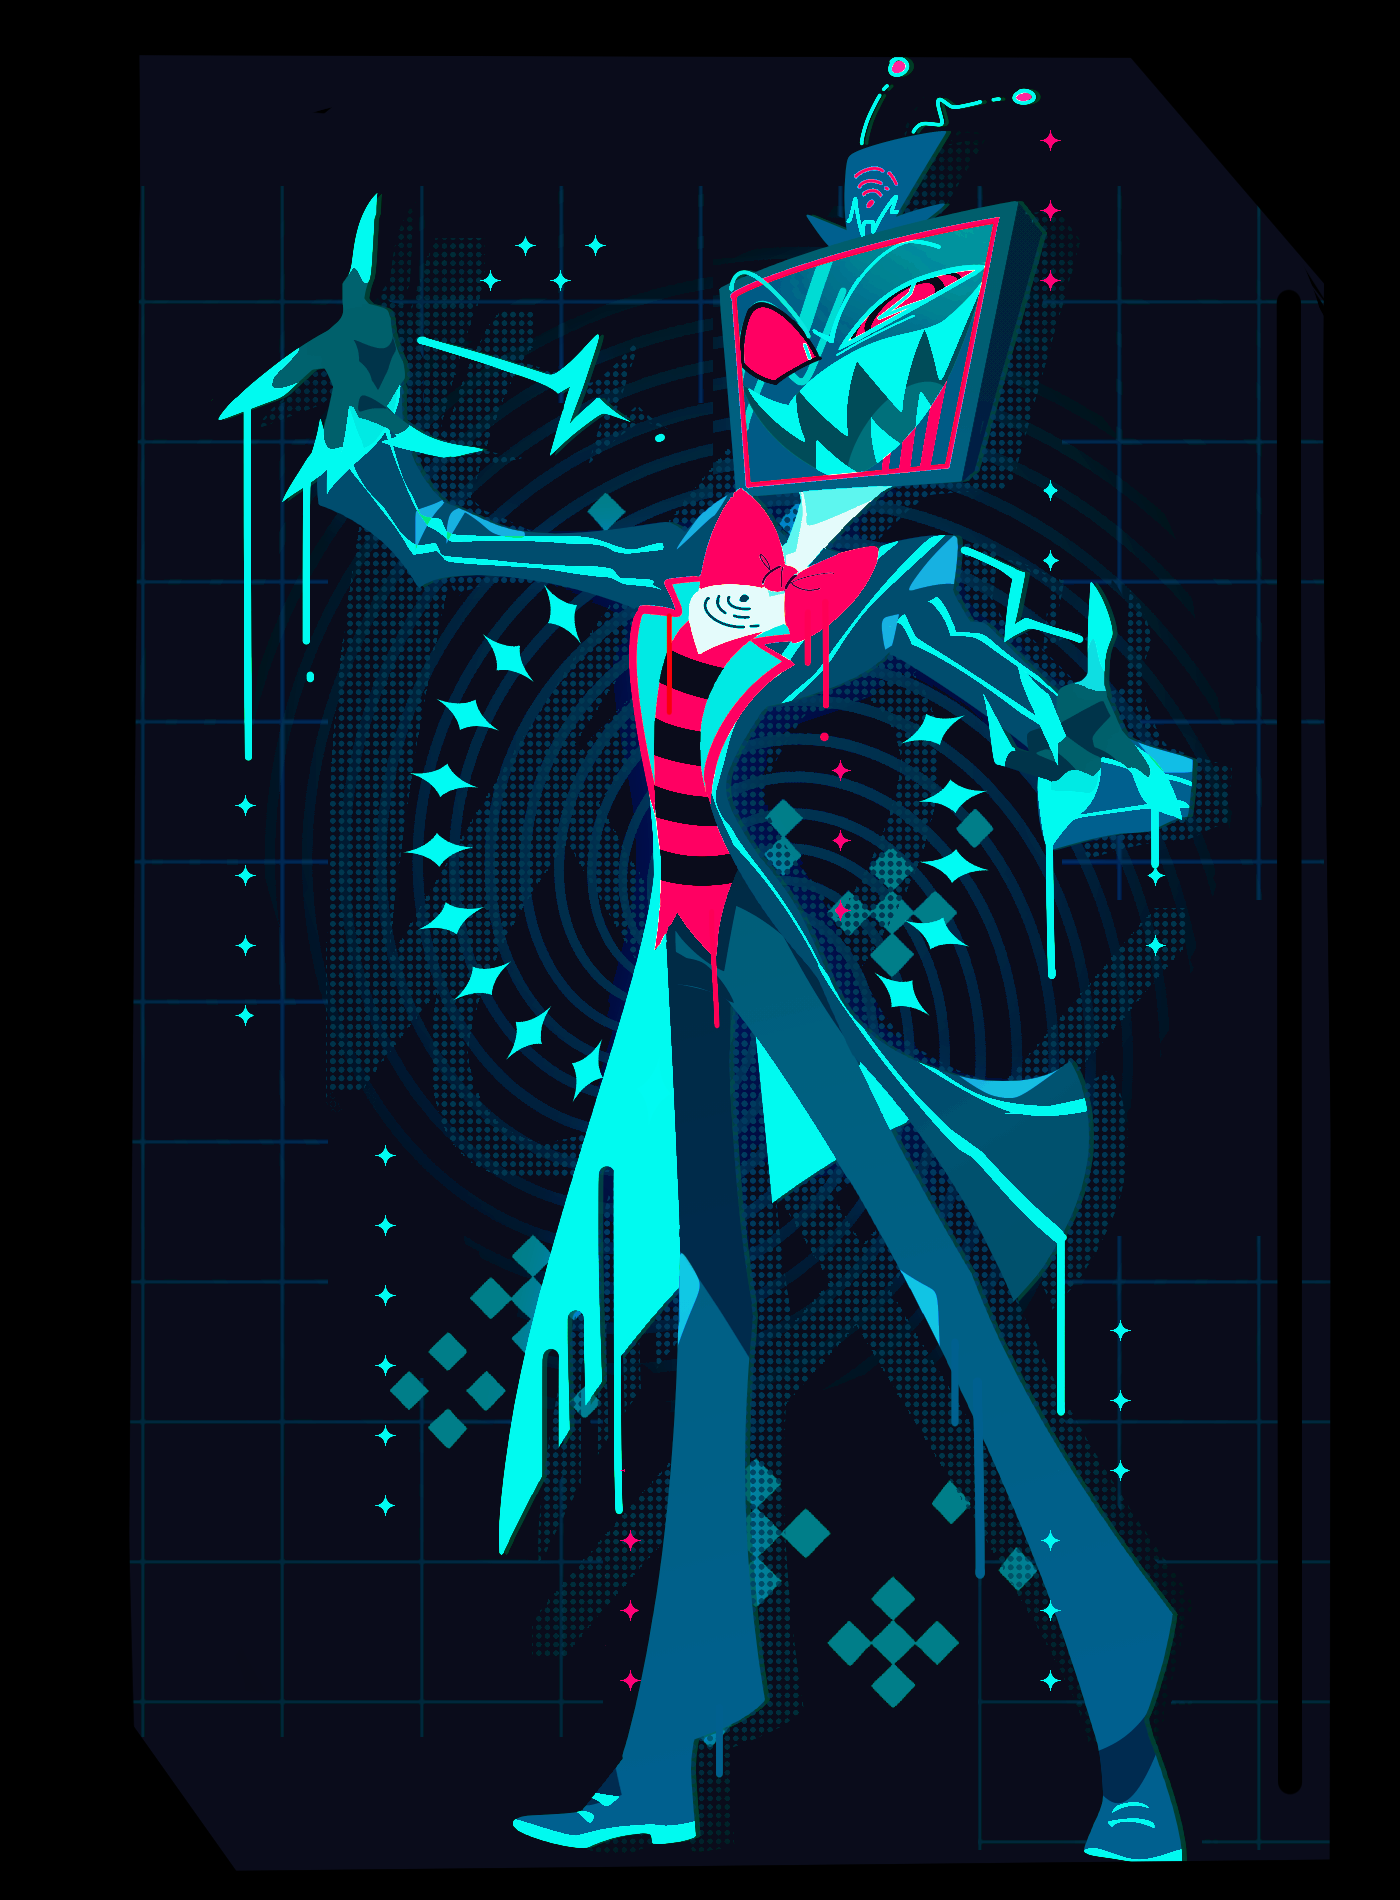
\includegraphics[width=\paperwidth,height=\paperheight]{vox.png}%
        }%
    }%
    \null
}{%
    \begin{center}
        \vspace*{\fill}
        {\Huge\bfseries Vox}\par
        \vspace{0.7cm}
        {\large Файл \texttt{vox.png} пока не найден.}\par
        \vspace*{\fill}
    \end{center}
}

\clearpage

% ============================================================
% Титульный лист
% ============================================================
\thispagestyle{empty}

\begin{center}
    {\large Московский физико-технический институт}\par
    \vspace{0.25cm}
    {\large Физтех-школа прикладной математики и информатики}\par

    \vfill

    {\Huge\bfseries Технологии программирования}\par
    \vspace{0.45cm}
    {\LARGE\bfseries и язык C++}\par

    \vspace{1.2cm}

    {\large Подробный конспект курса}\par
    \vspace{0.25cm}
    {\large C++17 с отдельными элементами C++20}\par

    \vfill

    \begin{tabular}{rl}
        Авторы: & Хомченко Илья \\
                & Шелегеда Наталья
    \end{tabular}

    \vfill

    {\large Москва, 2026}\par
\end{center}

\clearpage

% ============================================================
% Оглавление
% ============================================================
\tableofcontents
\clearpage

% ============================================================
% Все 15 завершённых лекций подключены ниже.
% ============================================================

\section*{О конспекте}
\addcontentsline{toc}{section}{О конспекте}

Этот конспект посвящён технологиям программирования и языку C++.
Основной стандарт курса --- C++17; заключительный блок отдельно показывает,
что меняют ключевые возможности C++20 и как они продолжают уже изученную модель языка.

Материал организован в 15 последовательных лекционных блоков с практическими
экспериментами. Код, сборка, работа компилятора, модель памяти, инструменты
разработки и производительность рассматриваются вместе, а не как независимые темы.


% Подключённые готовые лекции.
\section{Лекция 1. Введение в C++ и первая программа}
\label{sec:lecture-01}

Первая лекция нужна не для того, чтобы выучить много синтаксиса.
Наша задача --- построить правильную картину: что такое исходный
код, кто превращает его в исполняемую программу, зачем языку типы и как уже
на первом занятии пользоваться простыми полезными абстракциями стандартной
библиотеки.

\begin{importantbox}[Что нужно уметь после лекции]
Создать файл \texttt{.cpp}, собрать его через \texttt{g++}, запустить программу,
объяснить каждую строку простого \texttt{main}, пользоваться базовыми типами,
понимать целочисленное деление и простые неявные преобразования, а также
использовать \texttt{std::string}, \texttt{std::vector} и \texttt{std::map}
на уровне их основного контракта.
\end{importantbox}

\subsection{От задачи к машинному коду}

Процессор не выполняет строку

\begin{cppcodeplain}
std::cout << "Hello!\n";
\end{cppcodeplain}

непосредственно. В конечном счёте он исполняет машинные инструкции конкретной
архитектуры. Язык программирования позволяет описывать вычисление на более
высоком уровне: через типы, операции, функции и готовые абстракции.

\begin{definition}
\textbf{Исходный код} --- текст программы, написанный программистом.
Для C++ исходные файлы часто имеют расширение \texttt{.cpp}.
\end{definition}

\begin{definition}
\textbf{Компилятор} --- программа, которая анализирует исходный код и переводит
его в другую форму. В типичном C++ toolchain результат нескольких стадий
становится машинным кодом для выбранной платформы.
\end{definition}

\begin{whybox}[Компилятор против интерпретатора]
Деление языков на «компилируемые» и «интерпретируемые» работает только как
первое приближение. Реальные реализации могут использовать байткод, JIT и
смешанные схемы. Для нас важно, что обычная C++-сборка заранее создаёт
нативный executable, а компилятор получает информацию о типах до запуска.
\end{whybox}

\subsection{Почему C++}

C++ интересен сочетанием высокоуровневых абстракций и достаточно прямого
контроля над стоимостью программы. Можно говорить «динамическая
последовательность чисел» через \texttt{std::vector}, а позже при
необходимости разбираться с размещением памяти, временем жизни и машинным
кодом.

\begin{performancebox}
Нельзя делать вывод «программа быстрая, потому что она написана на C++».
Скорость зависит от алгоритма, структуры данных, аллокаций, кэшей,
оптимизатора, ввода-вывода и железа. Полезная идея C++ --- абстракция
не обязана означать большую runtime-стоимость.
\end{performancebox}

\subsection{Практический pipeline сборки}

Одна команда

\begin{shellcode}
g++ main.cpp -o program
\end{shellcode}

скрывает несколько разных этапов. Для обучения удобно видеть цепочку

\begin{center}
\texttt{main.cpp}
$\rightarrow$
\texttt{preprocessing}
$\rightarrow$
\texttt{assembly}
$\rightarrow$
\texttt{object file}
$\rightarrow$
\texttt{linking}
$\rightarrow$
\texttt{executable}.
\end{center}

\subsubsection{Preprocessing}

До основной компиляции обрабатываются директивы препроцессора, например

\begin{cppcodeplain}
#include <iostream>
\end{cppcodeplain}

На первом уровне понимания этого достаточно: после обработки заголовка
объявления стандартного потокового ввода-вывода становятся доступны текущей
единице трансляции.

\begin{mistakebox}[Что не надо говорить]
Фраза «\texttt{\#include} подключает библиотеку» смешивает разные стадии.
Заголовок участвует в preprocessing, а связывание с уже скомпилированным кодом
происходит на стадии linking.
\end{mistakebox}

\subsubsection{Object file и linker}

После анализа C++ компилятор может сгенерировать assembly, а assembler ---
объектный файл. Объектный файл уже содержит машинный код, но часто ещё имеет
неразрешённые ссылки на другие части программы и библиотеки.

\begin{definition}
\textbf{Линкер} связывает объектные файлы и библиотеки, разрешает внешние ссылки
и создаёт итоговый executable или библиотеку.
\end{definition}

\begin{standardbox}
Стандарт C++ определяет translation units и фазы трансляции, но не требует,
чтобы реализация буквально сохраняла промежуточные \texttt{.ii},
\texttt{.s} и \texttt{.o}. Мы создаём их специально, чтобы увидеть устройство
конкретного toolchain.
\end{standardbox}

\begin{practicebox}[Эксперимент 1: разобрать сборку по частям]
Файл \texttt{examples/01\_intro\_and\_first\_program/01\_compilation\_pipeline/inspect.sh}
отдельно запускает preprocessing, генерацию assembly, создание object file и
linking. После эксперимента команда \texttt{g++} перестаёт быть магической
кнопкой.
\end{practicebox}

\subsection{Hello, World! по строкам}

\begin{cppcode}
#include <iostream>

int main() {
    std::cout << "Hello, World!\n";
    return 0;
}
\end{cppcode}

\texttt{\#include <iostream>} --- директива preprocessing.
Заголовок \texttt{iostream} предоставляет интерфейс стандартных потоков.

\texttt{main} --- особая функция обычной C++-программы: с неё начинается
выполнение пользовательского кода после необходимой работы среды выполнения.

Слово \texttt{int} означает, что функция возвращает целое значение.
Для \texttt{main} это код завершения программы.

\texttt{std::cout} --- стандартный поток вывода. Префикс \texttt{std::}
указывает пространство имён стандартной библиотеки.

\begin{warningbox}[Почему сразу пишем std::]
В старых учебных примерах часто встречается \texttt{using namespace std;}.
Конструкция допустима, но как основной стиль она скрывает происхождение имён
и может создавать конфликты. В этом конспекте стандартные имена по умолчанию
пишутся явно: \texttt{std::cout}, \texttt{std::string}, \texttt{std::vector}.
\end{warningbox}

Оператор \texttt{<<} передаёт значение в поток вывода. Позже мы увидим, что
это перегруженный оператор; пока важен его контракт.

Текст в двойных кавычках --- строковый литерал.
Последовательность \texttt{\textbackslash n} обозначает перевод строки.

\texttt{return 0;} завершает функцию и сообщает об успешном завершении.
Достижение конца \texttt{main} без явного \texttt{return} также считается
успешным, но на первых примерах оставим возврат видимым.

\subsection{Первая команда компиляции}

\begin{shellcode}
g++ -std=c++17 -Wall -Wextra -Wpedantic hello.cpp -o hello
\end{shellcode}

Здесь:

\textbf{\texttt{g++}:} C++-драйвер GCC; \textbf{\texttt{-std=c++17}:} используем стандарт C++17; \textbf{\texttt{-Wall}:} включаем большой набор полезных предупреждений; \textbf{\texttt{-Wextra}:} включаем дополнительные предупреждения; \textbf{\texttt{-Wpedantic}:} просим предупреждать об отклонениях от стандарта; \textbf{\texttt{-o hello}:} задаём имя результата.

\begin{warningbox}
Название \texttt{-Wall} не означает буквально «все предупреждения GCC».
Поэтому полезные группы warnings часто комбинируют.
\end{warningbox}

Запуск в Linux:

\begin{shellcode}
./hello
\end{shellcode}

Префикс \texttt{./} явно указывает текущий каталог. Обычно shell ищет команды
в каталогах из \texttt{PATH}, а текущий каталог туда не включён.

\subsection{Из чего состоит строка C++}

Рассмотрим

\begin{cppcodeplain}
int age = 20;
\end{cppcodeplain}

\texttt{int} --- keyword, \texttt{age} --- identifier,
\texttt{20} --- literal, \texttt{=} --- operator,
\texttt{;} --- punctuation.

Комментарии нужны для неочевидной причины, а не для пересказа кода.

\begin{cppcodeplain}
// Плохо: увеличиваем count на один.
count += 1;
\end{cppcodeplain}

Хороший комментарий объясняет, почему увеличение происходит здесь или какой
инвариант мы поддерживаем.

\subsection{Типы как информация о значениях и операциях}

\begin{cppcode}
int age = 20;
double temperature = 36.6;
char grade = 'A';
bool passed = true;
\end{cppcode}

\begin{definition}
\textbf{Тип} определяет множество допустимых значений и операций, которые
имеют смысл для объекта или выражения.
\end{definition}

Тип нужен не только человеку: он сообщает компилятору, как трактовать данные,
какие операции разрешены и какие преобразования возможны.

Для первой лекции достаточно знать группы:

\texttt{bool}; символьный \texttt{char}; целые \texttt{short}, \texttt{int}, \texttt{long}, \texttt{long long} и unsigned-варианты; \texttt{float}, \texttt{double}, \texttt{long double}.

\begin{standardbox}[Не запоминаем int = 4 байта как закон языка]
На современных desktop-системах это часто так, но стандарт не определяет
\texttt{int} фразой «четырёхбайтовое целое». Конкретный размер относится к
реализации и платформе.
\end{standardbox}

\begin{warningbox}[double не равен множеству вещественных чисел]
Floating-point хранит конечное множество представимых значений. Многие
десятичные дроби нельзя представить точно, поэтому появляются ошибки
округления. Подробно вернёмся к этому позже.
\end{warningbox}

\subsection{Инициализация и арифметика}

\begin{cppcode}
int count = 5;
double price{12.5};
\end{cppcode}

Фигурная инициализация полезна тем, что запрещает ряд сужающих преобразований,
например попытку записать \texttt{3.14} непосредственно в \texttt{int}.

Базовые арифметические операции:

\begin{cppcode}
int a = 10;
int b = 3;

int sum = a + b;       // 13
int product = a * b;   // 30
int quotient = a / b;  // 3
int rest = a % b;      // 1
\end{cppcode}

Самый важный ранний пример:

\begin{cppcode}
int x = 7 / 2;         // 3
double y = 7.0 / 2.0; // 3.5
\end{cppcode}

\begin{whybox}[Почему 7 / 2 даёт 3]
Оба операнда целые, поэтому выполняется целочисленное деление.
В \texttt{7.0 / 2.0} операнды floating-point, поэтому операция другая.
\end{whybox}

Ещё важнее:

\begin{cppcode}
int a = 1;
int b = 4;

double wrong = a / b;       // 0.0
double right = 1.0 * a / b; // 0.25
\end{cppcode}

В первой строке сначала вычисляется целочисленное \texttt{1 / 4}, получается
\texttt{0}, и только затем ноль превращается в \texttt{double}.
Тип переменной слева не меняет задним числом семантику выражения справа.

\subsection{Сравнения и простые преобразования}

Операторы \texttt{==}, \texttt{!=}, \texttt{<}, \texttt{<=}, \texttt{>},
\texttt{>=} дают значение типа \texttt{bool}.

\begin{cppcode}
int age = 20;
bool adult = age >= 18;
\end{cppcode}

C++ также выполняет неявные преобразования:

\begin{cppcode}
int whole = 5;
double real = whole;  // 5 -> 5.0
\end{cppcode}

Обратное направление может терять информацию:

\begin{cppcode}
double real = 3.9;
int whole = real;  // дробная часть теряется
\end{cppcode}

Неявное преобразование --- конкретная операция с правилами, а не «магическая
совместимость типов».

\subsection{Ввод и вывод}

\begin{cppcode}
#include <iostream>

int main() {
    int age{};

    std::cout << "Enter age: ";
    std::cin >> age;

    std::cout << "Age: " << age << '\n';
    return 0;
}
\end{cppcode}

\texttt{std::cin >> age} просит поток ввода разобрать следующее значение как
\texttt{int}. Обработку ошибочного ввода пока откладываем: для неё нужны
управляющие конструкции.

\subsection{Первая стандартная абстракция: std::string}

\begin{cppcode}
#include <string>

std::string language{"C++"};
std::cout << language << '\n';
std::cout << language.size() << '\n';
\end{cppcode}

Пока читаем \texttt{language.size()} как «спросить у объекта длину».
Полный механизм методов появится вместе с классами.

\subsection{std::vector: последовательность однотипных значений}

\begin{cppcode}
#include <vector>

std::vector<int> numbers{10, 20, 30};

std::cout << numbers[0] << '\n';
std::cout << numbers.size() << '\n';

numbers.push_back(40);
\end{cppcode}

\texttt{std::vector<int>} пока читаем буквально как
«vector, элементы которого имеют тип int». Почему тип записан в угловых
скобках, объяснит лекция о шаблонах.

\begin{importantbox}
\texttt{vector} даёт абстракцию изменяемой последовательности однотипных
элементов и сам управляет необходимыми ресурсами. Поэтому мы можем решать
задачи с последовательностями до изучения ручного управления памятью.
\end{importantbox}

Индексация начинается с нуля. \texttt{operator[]} не проверяет границы
автоматически; к последствиям вернёмся в лекции о памяти.

\subsection{std::map: ключ и значение}

\begin{cppcode}
#include <map>
#include <string>

std::map<std::string, int> frequency;

frequency["cat"] += 1;
frequency["dog"] += 1;
frequency["cat"] += 1;

std::cout << frequency["cat"] << '\n'; // 2
\end{cppcode}

\texttt{std::map<std::string, int>} читаем как соответствие
«ключ типа string $\rightarrow$ значение типа int».

\begin{whybox}[Почему новый счётчик начинается с нуля]
\texttt{map::operator[]} при отсутствии ключа создаёт для него значение.
Для \texttt{int} значение по умолчанию равно нулю, после чего
\texttt{+= 1} увеличивает счётчик.
\end{whybox}

\subsection{Не смешиваем язык, библиотеку и инструменты}

Уже сейчас существуют три разных уровня:

\textbf{Язык C++:} типы, выражения, функции, синтаксис и правила преобразований; \textbf{Стандартная библиотека:} \texttt{iostream}, \texttt{string}, \texttt{vector}, \texttt{map}; \textbf{Toolchain:} \texttt{g++}, assembler, linker, CMake, shell.

\texttt{vector} не ключевое слово языка.
Флаг \texttt{-Wall} не входит в стандарт C++.
CMake --- не компилятор.

\subsection{CMake как первая абстракция над сборкой}

Для одного файла удобно написать команду \texttt{g++}. Когда исходников и
настроек становится больше, выгоднее описать цель сборки.

\begin{cmakecode}
cmake_minimum_required(VERSION 3.16)

project(basic_abstractions LANGUAGES CXX)

add_executable(basic_abstractions main.cpp)

target_compile_features(basic_abstractions PRIVATE cxx_std_17)
\end{cmakecode}

\texttt{add\_executable} создаёт build target, а
\texttt{target\_compile\_features} задаёт требование конкретно для него.

Сборка:

\begin{shellcode}
cmake -S . -B build
cmake --build build
./build/basic_abstractions
\end{shellcode}

\texttt{-S .} задаёт каталог исходников, \texttt{-B build} --- отдельный
каталог генерируемых файлов.

\begin{practicebox}[Эксперимент 2: простые абстракции]
Программа в
\texttt{examples/01\_intro\_and\_first\_program/02\_basic\_abstractions}
использует \texttt{string}, \texttt{vector} и \texttt{map}, но специально
обходится без циклов, собственных функций, указателей и классов.
Так мы начинаем с небольшого числа уже понятных абстракций.
\end{practicebox}

\subsection{Что пока остаётся за кадром}

Мы ещё не разобрали declaration и definition, scope, условия и циклы,
категории ошибок, память и lifetime, устройство \texttt{vector},
шаблоны, классы и стоимость операций контейнеров.

Это не пробел, а карта следующих лекций.

\subsection{Проверка понимания}

После лекции нужно суметь без подсказки объяснить:

1) чем исходный файл отличается от executable; 2) зачем нужны compiler и linker; 3) что делает \texttt{\#include}; 4) почему пишется \texttt{std::cout}; 5) почему \texttt{7 / 2} не равно \texttt{3.5}; 6) что означает \texttt{std::vector<int>}; 7) что означает \texttt{std::map<std::string, int>}; 8) почему новый \texttt{map}-счётчик можно увеличить через \texttt{+= 1}; 9) чем CMake отличается от компилятора.

\subsection{Источники для сверки}

Для терминов языка и фаз трансляции используем рабочий draft C++17 N4659.
Практический GCC pipeline сверяем с \textit{An Introduction to GCC}.
Первое педагогическое объяснение compilation pipeline сопоставляем с MIT
6.096 Lecture 1. Target-based сборку сверяем с \textit{Modern CMake}.

% Lecture 02: Объявления, управление потоком и ошибки

\section{Лекция 2. Объявления, поток управления и ошибки}
\label{sec:lecture-02}

Первая программа выполняла почти прямую последовательность команд. Реальная
программа должна хранить состояние, принимать решения, повторять действия и
останавливаться при нужном условии. Поэтому поток управления --- не набор
отдельных ключевых слов, а способ записать алгоритм.

\begin{importantbox}[Что нужно уметь после лекции]
Объявлять и инициализировать простые локальные объекты, строить выражения,
писать ветвления и циклы, проверять ввод, объяснять область видимости и
различать compile-time, linker, runtime, logic errors и undefined behavior.
Итоговая практическая цель --- небольшой корректный консольный инструмент.
\end{importantbox}

\subsection{Имя, объект, значение и состояние}

\begin{cppcode}
int attempts{0};
bool running{true};
double threshold{2.5};
char command{'s'};
\end{cppcode}

\begin{definition}
\textbf{Identifier} --- имя, которым исходный код обозначает сущность.
В примере это \texttt{attempts}, \texttt{running}, \texttt{threshold} и
\texttt{command}. Имя не может начинаться с цифры и не должно совпадать с
ключевым словом.
\end{definition}

\begin{definition}
\textbf{Объект} в терминологии C++ --- область хранения с типом и временем
жизни. \textbf{Значение} --- информация, которую выражение вычисляет или
объект хранит. Переменной будем называть именованный объект, значение которого
можно менять.
\end{definition}

Это точнее бытовой фразы «переменная --- коробка». Коробка полезна как первая
модель, но стандарт не обещает, что локальный объект обязательно лежит в CPU
stack: оптимизатор может держать значение в регистре или вообще устранить
отдельное хранение, сохранив наблюдаемое поведение программы.

Тип \texttt{int} хранит целые из диапазона, зависящего от реализации;
стандарт не обещает ему ровно четыре байта. \texttt{double} --- один из
floating-point типов, а не точные вещественные числа. \texttt{char} хранит
символьные/малые целочисленные значения, \texttt{bool} --- \texttt{false} или
\texttt{true}. Этих фундаментальных типов достаточно для текущих алгоритмов.

\subsection{Declaration, definition, initialization, assignment}

\begin{definition}
\textbf{Declaration} сообщает компилятору имя и свойства сущности. Definition
--- объявление, которое вводит саму сущность; для
обычного локального объекта definition предоставляет хранение.
\end{definition}

\begin{cppcode}
int score{10};       // definition и initialization
score = 12;          // assignment уже существующему объекту
extern int total;    // declaration; definition может быть в другом .cpp
\end{cppcode}

Инициализация создаёт начальное значение в момент начала lifetime объекта.
Присваивание заменяет значение уже живого объекта. Поэтому слова
«инициализируем второй раз» для \texttt{score = 12} неверны.

Основные формы, достаточные сейчас:

\begin{cppcode}
int a = 3;     // copy-initialization
int b(3);      // direct-initialization
int c{3};      // direct-list-initialization
int count{};   // value-initialization: для int получаем 0
\end{cppcode}

Фигурная форма хорошо видит некоторые narrowing conversions:

\begin{cppcode}
int truncated = 3.9; // допустимо с потерей дробной части; warning зависит от флагов
// int rejected{3.9}; // ошибка: list-initialization запрещает narrowing
\end{cppcode}

Не нужно превращать выбор скобок в догму. В учебных локальных объектах
\texttt{\{\}} явно показывает инициализацию и защищает от части сужений.

\begin{cppcode}
const int block_count{15};
// block_count = 16; // compile-time error
\end{cppcode}

\texttt{const} означает, что через это имя нельзя менять объект после
инициализации. Это полезный контракт намерения, а не обещание разместить число
в особой физической памяти.

\subsection{Литералы, выражения и преобразования}

Литерал записывает значение прямо в исходнике: \texttt{42}, \texttt{3.5},
\texttt{'q'}, \texttt{true}. Выражение сочетает литералы, имена и операторы и
вычисляет значение:

\begin{cppcode}
int completed{7};
int total{15};
int remaining = total - completed;
bool finished = remaining == 0;
\end{cppcode}

Арифметика использует \texttt{+}, \texttt{-}, \texttt{*}, \texttt{/} и для
целых \texttt{\%}. При \texttt{7 / 2} оба операнда целые, результат равен 3.
В \texttt{7.0 / 2} целое 2 преобразуется к floating-point, результат 3.5.

\begin{cppcode}
int part{1};
int whole{4};
double wrong = part / whole;       // сначала integer 0, затем double 0.0
double right = 1.0 * part / whole; // 0.25
\end{cppcode}

Неявное \texttt{int} $\rightarrow$ \texttt{double} удобно, но некоторые
большие целые представляются неточно. Обратное преобразование отбрасывает
дробную часть; слишком большое floating-point значение для целевого целого
типа может привести к undefined behavior. Сужение лучше делать заметным и
предварительно проверять диапазон. Подробные casts появятся позже.

Операторы \texttt{==}, \texttt{!=}, \texttt{<}, \texttt{<=}, \texttt{>},
\texttt{>=} возвращают \texttt{bool}. Логические \texttt{\&\&},
\texttt{||}, \texttt{!} означают «и», «или», «не»:

\begin{cppcode}
const bool valid_number = number >= 1 && number <= 15;
const bool should_print = show_all || !pair_complete;
\end{cppcode}

\subsubsection{Short-circuit --- не только оптимизация}

Для \texttt{left \&\& right} правый операнд вычисляется только если левый
оказался \texttt{true}. Для \texttt{left || right} --- только если левый
оказался \texttt{false}. Это гарантия языка и способ безопасно поставить
проверку перед опасной операцией:

\begin{cppcode}
const bool ratio_is_large = denominator != 0 && numerator / denominator > 2;
\end{cppcode}

Если знаменатель ноль, деление не выполняется. Переставить операнды нельзя:
integer division by zero имеет undefined behavior.

\subsection{Ветвление if: порядок проверок проектирует алгоритм}

\begin{cppcode}
if (score < 0) {
    std::cout << "invalid\n";
} else if (score < 50) {
    std::cout << "needs work\n";
} else {
    std::cout << "passed\n";
}
\end{cppcode}

Условия проверяются сверху вниз. Выполняется первое подходящее тело, остальные
ветви цепочки пропускаются. Значит, порядок влияет на корректность:
сначала часто ставят ошибки и более узкие случаи, затем общий случай.

Вложенный \texttt{if} нужен, когда второе решение имеет смысл только внутри
первого:

\begin{cppcode}
if (lecture_exists) {
    if (examples_exist) {
        std::cout << "complete pair\n";
    } else {
        std::cout << "examples missing\n";
    }
}
\end{cppcode}

Фигурные скобки синтаксически необязательны для одного statement, но в нашем
стиле ставятся всегда: добавление второй строки тогда не изменит границы ветви.

\begin{mistakebox}[Присваивание вместо сравнения]
\texttt{if (answer = 0)} присваивает ноль и затем преобразует результат к
\texttt{bool}; это корректный синтаксис, но почти наверняка logic error.
GCC с \texttt{-Wall -Wextra -Wpedantic} реально пишет warning вида
\texttt{suggest parentheses around assignment used as truth value}.
Нужное сравнение: \texttt{if (answer == 0)}.
\end{mistakebox}

Warning не обязан останавливать сборку и не доказывает
ошибки. Но его нужно прочитать и устранить или осознанно обосновать.

\subsection{switch: выбор по дискретному значению}

Меню естественно выражается через \texttt{switch}:

\begin{cppcode}
switch (choice) {
case 1:
    std::cout << "show all\n";
    break;
case 2:
    std::cout << "check one\n";
    break;
case 3:
case 4:
    std::cout << "report\n";
    break;
default:
    std::cout << "unknown command\n";
    break;
}
\end{cppcode}

Выражение \texttt{switch} вычисляется один раз, затем выбирается совпавший
\texttt{case}; \texttt{default} обрабатывает отсутствие совпадения.
\texttt{break} выходит из ближайшего \texttt{switch}. Без него выполнение
продолжается в следующий case --- это fallthrough. Иногда оно намеренно, как
для 3 и 4 выше. Если между непустыми case переход нужен специально, C++17
позволяет отметить его \texttt{[[fallthrough]];}.

\begin{implementationbox}
Компилятор может реализовать \texttt{switch} цепочкой сравнений, jump table
или иначе. Стандарт задаёт поведение, но не требует jump table. Выбираем
\texttt{switch} ради ясности дискретного выбора, не по легенде о скорости.
\end{implementationbox}

Для диапазонов и сложных независимых условий удобнее \texttt{if}; case labels
должны быть подходящими constant expressions и не могут означать диапазон.

\subsection{Циклы: повторение с условием остановки}

Перед циклом ответьте на четыре вопроса: какое состояние меняется, когда
продолжаем, какой шаг приближает остановку и что должно оставаться истинным.

\subsubsection{while и validation loop}

\begin{cppcode}
int number{};
while (!(std::cin >> number) || number < 1 || number > 15) {
    std::cout << "Enter an integer from 1 to 15: ";
    std::cin.clear();
    std::cin.ignore(std::numeric_limits<std::streamsize>::max(), '\n');
}
\end{cppcode}

\texttt{while} сначала проверяет условие, поэтому тело может не выполниться ни
разу. Здесь готовый stream API сообщает об ошибке ввода; \texttt{clear}
сбрасывает состояние ошибки, \texttt{ignore} удаляет неподходящий остаток
строки. Это validation loop: выход возможен только после допустимого значения.

\subsubsection{do while}

\begin{cppcode}
int choice{};
do {
    std::cout << "1 - continue, 0 - exit: ";
    std::cin >> choice;
} while (choice != 0);
\end{cppcode}

\texttt{do while} проверяет условие после тела, поэтому тело выполняется хотя
бы один раз. Это бывает естественно для показа меню, но если ввод может
сломаться, всё равно нужна явная обработка состояния потока.

\subsubsection{for и границы}

\begin{cppcode}
int sum{};                              // accumulator
for (int value = 1; value <= 5; ++value) {
    sum += value;
}
\end{cppcode}

Порядок таков: initialization выполняется один раз; condition проверяется
перед каждой итерацией; затем тело; iteration expression; новая проверка.
Переменная \texttt{value} видна в заголовке и теле, но после цикла её scope
заканчивается. \texttt{sum} --- accumulator: хранит результат уже обработанной
части. Переменная, считающая события, называется counter.

\begin{mistakebox}[Off-by-one]
Для значений 1, 2, 3, 4, 5 нужно \texttt{value <= 5}. Условие
\texttt{value < 5} выполнит четыре итерации. Для индексов последовательности,
напротив, обычно естествен полуинтервал \texttt{0 <= index < size}.
Проверяйте первую, последнюю и пустую итерации отдельно.
\end{mistakebox}

Если шаг не меняет состояние к остановке, например забыто \texttt{++value},
может возникнуть бесконечный цикл. Запись \texttt{while (true)} сама по себе
не ошибка: menu loop может завершаться явным \texttt{break}, но путь выхода
должен быть понятен.

\subsubsection{break, continue, sentinel и поиск}

\texttt{break} завершает ближайший цикл. \texttt{continue} пропускает остаток
текущей итерации и переходит к следующей проверке/шагу. Чрезмерное количество
таких переходов усложняет чтение, но для раннего отсева они полезны:

\begin{cppcode}
for (int value = 1; value <= 20; ++value) {
    if (value % 2 != 0) {
        continue;
    }
    if (value > 10) {
        std::cout << "first suitable: " << value << '\n';
        break;
    }
}
\end{cppcode}

Sentinel-controlled loop заканчивает последовательность по специальному
значению, которое не хранит данные:

\begin{cppcode}
int sum{};
int value{};
while (std::cin >> value && value != -1) {
    sum += value;
}
\end{cppcode}

Здесь \texttt{-1} --- sentinel. Short-circuit гарантирует: сравнение
выполняется только после успешного чтения. Так обрабатывается последовательность
неизвестной длины.

\subsubsection{Loop invariant --- человеческое доказательство}

Инвариант --- утверждение, истинное перед каждой итерацией. Для суммирования:
«\texttt{sum} равен сумме уже обработанных значений». Оно истинно до первой
итерации (обработанных значений нет, \texttt{sum == 0}); тело сохраняет его,
добавляя ровно текущее значение; вместе с условием выхода оно объясняет итог.
Это не формальная магия, а компактный способ проверить алгоритм.

\subsection{Block scope, shadowing и lifetime}

Фигурные скобки создают block scope:

\begin{cppcode}
int count{1};
if (count > 0) {
    int message_count{2};
    std::cout << message_count << '\n';
}
// message_count здесь не виден
\end{cppcode}

Scope отвечает, где имя можно использовать в тексте программы. Lifetime
отвечает, когда объект существует при выполнении. Для простого локального
объекта в блоке lifetime начинается после корректной инициализации и
заканчивается при выходе из блока; эти понятия связаны, но не одинаковы.

\begin{cppcode}
int status{1};
if (ready) {
    int status{2}; // shadowing: скрывает внешнее имя внутри блока
    std::cout << status << '\n';
}
\end{cppcode}

Shadowing допустим, но легко заставляет читать не тот \texttt{status}. В
обычном коде лучше выбрать другое имя. Компиляторы могут иметь отдельные
warnings для shadowing; базовые три флага не обязаны включать их все.

\subsection{Карта ошибок по pipeline}

\textbf{Compile-time error:} исходник не удовлетворяет правилам языка, например присваивание объекту \texttt{const}; executable не создаётся; \textbf{Linker error:} translation unit скомпилирован, но linker не нашёл definition объявленной сущности: обычное \texttt{undefined reference}. Это продолжает pipeline лекции~1; \textbf{Warning:} compiler сообщает о подозрительном, но обычно допустимом коде; сборка может продолжиться; \textbf{Runtime failure:} программа запустилась, но не смогла выполнить задачу: например, не найден корень курса или вход неожиданно закончился. Ненулевой exit status позволяет сообщить об этом окружению; \textbf{Logic error:} программа корректно компилируется и выполняется, но даёт неверный ответ, например сумма 1--5 вычисляется циклом \texttt{value < 5}; \textbf{Undefined behavior (UB):} стандарт не накладывает требований на поведение, например при signed integer overflow или integer division by zero. UB не обязано приводить к crash.

Implementation-defined behavior означает, что реализация выбирает один из
допустимых вариантов и документирует выбор (например, размер \texttt{int}).
Unspecified behavior также допускает несколько вариантов, но реализация не
обязана документировать выбор. Это не синонимы UB.

\begin{ubbox}[Почему «у меня работает» недостаточно]
Неправильная программа с UB может напечатать ожидаемое число, упасть или
изменить поведение после оптимизации. Проверять нужно правила операции, а не
только один запуск на одной машине.
\end{ubbox}

\subsection{Diagnostics: compiler и sanitizer решают разные задачи}

Для GCC и Clang используем минимум:

\begin{shellcode}
g++ -std=c++17 -Wall -Wextra -Wpedantic program.cpp -o program
\end{shellcode}

Компилятор обязан диагностировать некоторые нарушения, а warnings помогают
найти дополнительные подозрительные места. Но корректная сборка не доказывает
корректность алгоритма.

UndefinedBehaviorSanitizer добавляет runtime-проверки некоторых классов UB:

\begin{shellcode}
g++ -std=c++17 -fsanitize=undefined \
    -fno-sanitize-recover=undefined program.cpp -o program
./program
\end{shellcode}

Это режим конкретного toolchain, а не часть стандарта C++. Он видит только
проверяемые события реально пройденного пути. Отсутствие diagnostics не
доказывает отсутствие UB во всей программе.

\subsection{Эксперимент 1: course\_status}

Инструмент
\texttt{examples/02\_declarations\_flow\_and\_errors/01\_course\_status}
read-only проверяет все 15 известных пар
\texttt{lectures/NN\_slug.tex} $\leftrightarrow$
\texttt{examples/NN\_slug/}. Он ищет корень курса от текущего каталога вверх,
но ничего не создаёт, не удаляет и не переписывает.

\begin{shellcode}
cmake -S examples/02_declarations_flow_and_errors/01_course_status \
      -B examples/02_declarations_flow_and_errors/01_course_status/build
cmake --build examples/02_declarations_flow_and_errors/01_course_status/build
./examples/02_declarations_flow_and_errors/01_course_status/build/course_status
\end{shellcode}

Программа хранит \texttt{running} и выбранный пункт меню. Внешний
\texttt{while} повторяет меню, \texttt{switch} выбирает действие, а
\texttt{for} проверяет 15 пар. Результаты двух проверок имеют тип
\texttt{bool}; локальные блоки case
ограничивают scope временных имён. \texttt{continue} возвращает к меню после
плохого ввода, \texttt{break} завершает case. Штатный выход имеет status 0,
невозможность найти корень --- 2.

\begin{standardbox}[Язык и библиотека не смешиваем]
\texttt{if}, \texttt{switch}, \texttt{while}, \texttt{for} и scope --- тема
языка этой лекции. \texttt{std::filesystem} --- готовый library API C++17,
которым мы спрашиваем о путях; внутреннее устройство API сейчас не изучаем.
\end{standardbox}

Правильный результат: пункты 1 и 2 сообщают реальное состояние файлов, пункт
3 показывает только неполные пары (для утверждённой структуры их нет), буква
вместо номера не ломает menu loop, 0 завершает программу.

\subsection{Эксперимент 2: control flow и реальные diagnostics}

Второй каталог блока, \texttt{02\_control\_flow\_lab}, содержит несколько
маленьких cases вместо одного искусственного файла.

\begin{shellcode}
printf 'y\n' | \
  examples/02_declarations_flow_and_errors/02_control_flow_lab/run_lab.sh
\end{shellcode}

Лаборатория реально проверяет три ветви \texttt{if}, границу цикла и
short-circuit. Затем она ожидает: ненулевой exit status у демонстрации logic
error; warning для assignment в условии; отказ компиляции при изменении
\texttt{const}; runtime-диагностику UBSan для signed overflow. Expected failure
--- PASS только когда log содержит именно ожидаемую причину. Полные сообщения
конкретного установленного компилятора сохраняются в локальном
\texttt{generated/} и не выдаются за универсальный текст стандарта.

\subsection{Сильные стороны и цена свободы}

C++ прямо выражает control flow, а информация о типах позволяет найти много
ошибок до запуска. Состояние и шаги алгоритма видны в коде; стандартная
библиотека даёт готовые абстракции вроде streams, vector и filesystem. Один
исходник можно собирать в обычном режиме, с усиленными warnings или sanitizer.

Цена этой свободы технически существенна: implicit conversions способны
терять данные; logic errors compiler находить не обязан; некоторые неверные
программы успешно компилируются; язык допускает UB. Поэтому программист
отвечает за условия операций, границы циклов, progress к остановке и проверку
диагностик.

\subsection{Проверка понимания}

После лекции нужно уметь без подсказки:

1) отличить initialization от assignment и declaration от definition; 2) объяснить тип результата сравнения и short-circuit; 3) выбрать \texttt{if} или \texttt{switch} и обосновать порядок проверок; 4) записать validation, sentinel и menu loops; 5) назвать initialization, condition, body и iteration expression цикла; 6) найти off-by-one и сформулировать простой loop invariant; 7) отличить scope от lifetime и заметить shadowing; 8) классифицировать compile, link, runtime, logic errors и UB; 9) объяснить, почему warnings и sanitizer полезны, но не доказывают корректность; 10) написать небольшую консольную программу с корректным exit status.

\subsection{Источники для сверки}

Правила declarations, statements, conversions и undefined behavior сверены с
рабочим draft C++17 N4659. Педагогический порядок условий и циклов сопоставлен
с MIT 6.096 Lecture 2, но старый стиль примеров заменён современным явным
\texttt{std::} и фигурными скобками. Практика warnings и стадий сборки сверена
с \textit{An Introduction to GCC}; target-based сборка продолжает подход
первой лекции и \textit{Modern CMake}.

% Lecture 03: Указатели, память и массивы

\section{Лекция 3. Указатели, память и массивы}
\label{sec:lecture-03}

В предыдущей лекции объект хранил одно значение, а цикл повторял действие.
Теперь нужно хранить несколько однотипных объектов подряд и понимать их
адреса. Сначала построим честную модель raw array и указателя, затем увидим,
какую ручную работу снимают \texttt{std::array} и \texttt{std::vector}.

\begin{importantbox}[Главный вопрос]
Что означает «несколько объектов подряд в памяти», почему возникает pointer
arithmetic и почему для обычного изменяемого набора данных современный C++
чаще выбирает \texttt{std::vector}?
\end{importantbox}

\subsection{Объект, storage, lifetime и адрес}

Уточним три разных понятия: \emph{storage} --- память, достаточно большая и
правильно выровненная для объекта; \emph{object lifetime} --- интервал
выполнения, в котором объект существует; \emph{value} --- информация, которую
он хранит. Storage само по себе ещё не всегда означает живой объект. Для
обычного локального объекта lifetime начинается после инициализации и
заканчивается при выходе из блока.

\begin{cppcode}
int score{42};
std::cout << score << '\n';   // значение
std::cout << &score << '\n';  // адрес объекта
\end{cppcode}

\begin{definition}
\textbf{Адрес} --- значение, обозначающее положение объекта или функции в
абстрактной модели C++. Указатель может хранить такое значение.
\end{definition}

Выведенный адрес помогает наблюдать взаимное размещение, но его нельзя без
оговорки называть физическим адресом RAM. Automatic storage duration также не
обязывает реализацию держать объект на CPU stack: это обычная реализация, а
не требование стандарта.

\texttt{sizeof(expression)} даёт размер представления в байтах типа
\texttt{std::size\_t}. Байт C++ равен размеру \texttt{char} и содержит не
менее восьми бит; универсального обещания ровно восьми бит нет. Обычно операнд
\texttt{sizeof} не вычисляется. Результат «\texttt{int} равен 4 байтам» можно
наблюдать на машине, но нельзя превращать в закон языка. Alignment означает,
что адрес некоторых типов должен быть подходяще выровнен; компилятор учитывает
это при размещении, подробности сейчас не нужны.

\subsection{Pointer basics: адрес и значение по адресу}

\begin{cppcode}
int score{42};
int* pointer{&score};

std::cout << pointer << '\n';   // pointer value: адрес score
std::cout << *pointer << '\n';  // pointed-to value: 42
*pointer = 50;                  // меняет score
\end{cppcode}

\texttt{int* pointer} объявляет объект типа «pointer to \texttt{int}».
Звёздочка в declaration участвует в записи типа; \texttt{*pointer} в
expression выполняет \emph{dereference}. Оператор \texttt{\&score} берёт
адрес. Pointer --- не «просто integer»: у него отдельный тип, допустимые
операции и правила действительности.

\begin{whybox}[Зачем различать pointer и pointed-to value]
Копирование \texttt{pointer} копирует адресное значение, не \texttt{score}.
Присваивание \texttt{*pointer = 50} работает с объектом по адресу.
\end{whybox}

Минимальный \texttt{const} для чтения без изменения:

\begin{cppcode}
int score{42};
const int* view{&score};
// *view = 50; // compile-time error
\end{cppcode}

Сам \texttt{view} можно направить на другой \texttt{int}. Полная система
const будет в следующем блоке.

\subsubsection{nullptr и действительность}

\texttt{nullptr} явно означает «сейчас не указывает на объект» и имеет
специальный тип. Старый литерал \texttt{0} не используем как основной стиль.

\begin{cppcode}
int* selected{nullptr};
if (selected != nullptr) {
    std::cout << *selected << '\n';
}
\end{cppcode}

Dereference требует подходящий живой объект. Проверка на \texttt{nullptr}
устраняет только null case, но не распознаёт dangling pointer.

\begin{definition}
\textbf{Dangling pointer} сохраняет адресное значение после окончания lifetime
объекта, на который раньше указывал. Доступ к прежнему объекту через него
недопустим.
\end{definition}

Неинициализированный локальный pointer фундаментального типа имеет
неопределённое значение; его использование может иметь undefined behavior.
Безопасная привычка --- сразу дать адрес живого объекта или \texttt{nullptr}.

\subsection{Raw array: фиксированная последовательность}

\begin{cppcode}
int temperatures[4]{18, 20, 21, 19};
\end{cppcode}

Это built-in, или raw, array из четырёх \texttt{int}. Extent \texttt{4}
входит в array type и известен при компиляции. Все элементы имеют один
тип, индексы идут от нуля, объекты расположены непрерывно без промежутков
между соседними элементами.

\begin{cppcode}
int values[4]{};          // все элементы равны нулю
int inferred[]{2, 4, 6}; // extent 3 выведен из initializer
int partial[4]{7, 8};    // 7, 8, 0, 0
values[0] = 10;
\end{cppcode}

Во время выполнения \texttt{values[i]} выбирает элемент, но built-in access
не вставляет обязательную проверку границ.

\begin{cppcode}
int values[]{10, 20, 30, 40};
const std::size_t count = sizeof(values) / sizeof(values[0]);
\end{cppcode}

\texttt{sizeof(values)} здесь означает весь array object, а
\texttt{sizeof(values[0])} --- элемент. Деление --- лишь локальный
учебным приёмом там, где expression всё ещё имеет array type.

\begin{ubbox}[Out-of-bounds]
Для extent $N$ действительны индексы от 0 до $N-1$. \texttt{values[N]} уже
за границей. Чтение или запись имеет UB. UB не обещает crash: возможны
правдоподобный вывод, повреждение состояния или иное поведение после
оптимизации.
\end{ubbox}

\subsection{Array-to-pointer conversion: массив не pointer}

\begin{cppcode}
int values[]{10, 20, 30, 40}; // type: int[4]
int* first{values};           // conversion; type: int*
\end{cppcode}

Array object и pointer object различны. У массива четыре элемента и fixed
extent; у \texttt{first} одно pointer value. Во многих expressions array
неявно преобразуется в pointer на первый элемент: при инициализации
\texttt{first}, в \texttt{values + 1} и при передаче обычному pointer
parameter. Функции подробно появятся в блоке~4.

Преобразование происходит не везде:

\begin{cppcode}
std::cout << sizeof(values) << '\n'; // весь int[4]
std::cout << sizeof(first) << '\n';  // один int*
std::cout << &values << '\n';        // pointer на whole array, другой тип
\end{cppcode}

После conversion pointer не несёт extent. Поэтому деление размера pointer на
размер элемента не находит длину исходного массива. Pointer можно
направить заново, имя массива --- нельзя; raw arrays также не присваиваются
целиком. Фраза «имя массива --- pointer» скрывает эти различия. Точно:
array expression во многих контекстах \emph{преобразуется} в pointer.

\subsection{Pointer arithmetic существует из-за массивов}

\begin{cppcode}
int values[]{10, 20, 30, 40};
int* p{values};
std::cout << *(p + 2) << '\n';
++p;
std::cout << p - values << '\n';
\end{cppcode}

Для \texttt{int*} операция \texttt{p + 1} означает следующий \texttt{int},
не следующий машинный байт. \texttt{a[i]} имеет семантику
\texttt{*(a + i)}. Вычитание pointers даёт число элементов типа
\texttt{std::ptrdiff\_t}, но оба должны относиться к одному array object.

\begin{cppcode}
int values[]{10, 20, 30, 40};
int* begin{values};
int* end{values + 4};
for (int* current = begin; current != end; ++current) {
    std::cout << *current << '\n';
}
\end{cppcode}

\texttt{end} --- one-past pointer: его разрешено сформировать и сравнить как
границу полуинтервала $[begin,end)$, но \texttt{*end} имеет UB. Нельзя уходить
дальше one-past или выполнять арифметику между несвязанными arrays.

\begin{performancebox}[Индекс или pointer increment?]
\texttt{a[i]} и \texttt{*(a + i)} выражают ту же адресацию. Нельзя обещать,
что одна запись быстрее: нужен benchmark или assembly для конкретных compiler,
flags и workload. В обычном коде выбираем ясность.
\end{performancebox}

\subsection{Коротко о C-style strings}

\begin{cppcode}
char label[]{'C', '+', '+', '\0'};
char same_label[]{"C++"};
\end{cppcode}

C-style string --- последовательность \texttt{char} с null terminator
\texttt{'\textbackslash 0'}. Extent второго массива равен 4, хотя видимых
символов три. Отсутствие terminator позволяет C API читать за границу. Для
совместимости такая форма важна, но основной текстовый тип курса ---
\texttt{std::string}.

\subsection{std::array: удобный fixed-size container}

\begin{cppcode}
#include <array>
std::array<int, 4> values{10, 20, 30, 40};
std::cout << values.size() << '\n';
std::cout << values[1] << ' ' << values.at(2) << '\n';
std::cout << values.data() << '\n';
\end{cppcode}

Размер входит в тип и не меняется runtime, storage contiguous.
Объект знает \texttt{size()}, копируется и присваивается целиком;
\texttt{at()} проверяет границу и при ошибке сообщает exception. Исключения
будут отдельной темой. \texttt{data()} даёт pointer на первый элемент, а
\texttt{begin()}/\texttt{end()} интуитивно обозначают начало и one-past;
iterators системно изучим позже.

\subsection{std::vector: dynamic size и владение storage}

Raw array не растёт. Ручной dynamic array потребовал бы получить новый
участок, перенести элементы и освободить старый на всех путях. Naked
\texttt{new[]} / \texttt{delete[]} сейчас не используем: управление
динамической памятью будет позже.

\begin{cppcode}
std::vector<int> values{10, 20, 30};
values.push_back(40);
std::cout << values.size() << ' ' << values.capacity() << '\n';
std::cout << values[0] << ' ' << values.at(3) << '\n';
\end{cppcode}

Vector владеет внутренним storage и управляет lifetime элементов. Элементы
contiguous, \texttt{data()} возвращает pointer на первый. \texttt{empty()}
проверяет нулевой size. \texttt{operator[]} требует правильной границы от
программиста; \texttt{at()} проверяет её.

\begin{definition}
\texttt{size()} --- число живых элементов. \texttt{capacity()} --- сколько
поместится в текущем storage без нового выделения. Capacity не меньше size,
но позиции между ними ещё не являются элементами.
\end{definition}

Когда capacity исчерпана, \texttt{push\_back} может сделать
\emph{reallocation}: получить больший contiguous участок, перенести элементы
и отказаться от старого. Точный коэффициент роста и layout не гарантированы.

\begin{cppcode}
std::vector<int> values{10};
int* old_data{values.data()};
const std::size_t old_capacity{values.capacity()};
while (values.capacity() == old_capacity) {
    values.push_back(20);
}
// old_data больше не dereference: reallocation его инвалидировал
\end{cppcode}

Элементы теперь живут в новом storage, поэтому старый адрес не обозначает
прежний живой объект. Reallocation инвалидирует pointers, references и
iterators на элементы. Последние два термина здесь лишь анонс будущих тем.

\begin{cppcode}
std::vector<int> values;
values.reserve(100);
std::cout << values.size();     // 0
std::cout << values.capacity(); // не меньше 100
\end{cppcode}

\texttt{reserve} подготавливает capacity, но не создаёт элементы и не меняет
logical size; это не \texttt{resize}. Он уменьшает число reallocations при
хорошем прогнозе, но сам способен инвалидировать старые pointers.

Один рост с reallocation стоит $O(n)$. Capacity растёт с запасом, поэтому
дорогая операция нужна не при каждом добавлении. \texttt{push\_back} имеет
amortized $O(1)$: постоянную среднюю стоимость на длинной серии, не гарантию
$O(1)$ каждого вызова.

\subsection{Raw array, std::array или std::vector?}

\begin{center}\small
\begin{tabularx}{\textwidth}{@{}lXXX@{}}
\toprule
Свойство & raw array & \texttt{std::array} & \texttt{std::vector} \\
\midrule
Размер & fixed & fixed, часть типа & dynamic \\
Знает размер & extent в array type & \texttt{size()} & \texttt{size()} \\
Checked access & нет & \texttt{at()} & \texttt{at()} \\
Copy/assignment & не целиком & целиком & целиком \\
Storage & contiguous & contiguous & contiguous \\
Pointer access & conversion & \texttt{data()} & \texttt{data()} \\
Обычная роль & ABI/C API, low-level & fixed container & растущая sequence \\
\bottomrule
\end{tabularx}
\end{center}

Raw arrays не запрещены: они раскрывают язык и нужны некоторым ABI,
embedded- и C interfaces. Для обычного владения fixed sequence удобнее
\texttt{std::array}, runtime-размером --- \texttt{std::vector}.

\subsection{Карта memory errors}

\textbf{Uninitialized pointer:} неопределённое значение адреса; \textbf{Null dereference:} \texttt{*nullptr} не обозначает объект и имеет UB; \textbf{Dangling/use-after-lifetime:} адрес сохранился после конца lifetime; \textbf{Out-of-bounds:} индекс или dereference вышел за элементы; \textbf{Invalid arithmetic:} pointer вышел за one-past одного массива или операция смешала несвязанные arrays; \textbf{Vector invalidation:} reallocation закончила lifetime элементов в старом storage, поэтому старый pointer нельзя dereference.

Scope отвечает, где имя доступно в тексте; lifetime --- когда объект
существует runtime. Вынос адреса за scope имени не продлевает lifetime.

\subsection{ASan и UBSan: наблюдаем часть UB}

AddressSanitizer добавляет runtime-проверки для части out-of-bounds,
use-after-free и use-after-scope. UndefinedBehaviorSanitizer проверяет часть
других UB. Это instrumentation toolchain, не изменение стандарта.

\begin{shellcode}
cmake -S . -B build-sanitize -DENABLE_SANITIZER_CASES=ON \
  -DCMAKE_BUILD_TYPE=Debug
cmake --build build-sanitize
./build-sanitize/raw_oob
\end{shellcode}

PASS требует реальных причин: stack-buffer-overflow, stack-use-after-scope и
heap-use-after-free для pointer после vector reallocation. Эти программы
намеренно имеют UB и изолированы от safe lab.

\begin{warningbox}[Sanitizer не доказывает корректность]
Instrumentation видит не все нарушения и только на выполненных путях.
Отсутствие сообщения не доказывает отсутствие UB.
\end{warningbox}

\subsection{Производительность без лозунгов}

Все три варианта дают contiguous элементы. Последовательный проход часто
помогает cache locality, но конкретный cache --- свойство реализации и
железа. Vector хранит metadata; обычно она мала, но стандарт не обещает layout
или число слов. Reallocation стоит $O(n)$, reserve может уменьшить allocations,
а проход по готовому vector может быть столь же cache-friendly, как по array.

Поэтому «vector медленнее массива» не универсально. Нужно назвать operation,
size, access pattern, compiler flags и платформу, затем измерить. Benchmark
здесь N/A: лаборатория наблюдает семантику storage, не выдаёт нестабильные
наносекунды за закон.

\subsection{Эксперимент 1: course\_inventory}

Read-only утилита в
\texttt{examples/03\_pointers\_memory\_and\_arrays/01\_course\_inventory}
проходит по фиксированным 15 slugs в \texttt{std::array}, реально проверяет
lecture file/examples directory, считает байты, строки и обычные файлы.
Измеренные строки собираются в \texttt{std::vector<BlockInfo>}.

Адреса \texttt{blocks.data()} и \texttt{rows.data()} наблюдают начало двух
contiguous областей, но не физический RAM address. Fixed input и dynamic
results показывают выбор контейнера; reserve меняет capacity, не size.

\begin{shellcode}
cd examples/03_pointers_memory_and_arrays/01_course_inventory
cmake -S . -B build
cmake --build build
./build/course_inventory --root ../../..
./build/course_inventory --root ../../.. --block 3
ctest --test-dir build --output-on-failure
\end{shellcode}

PASS: вывод основан на текущих файлах, totals согласованы, один блок и все
блоки завершаются с exit code 0. Утилита ничего не изменяет.

\subsection{Эксперимент 2: array\_vs\_vector\_lab}

Safe executable показывает адреса raw array, оба \texttt{sizeof}, conversion,
pointer arithmetic и one-past без dereference; затем fixed
\texttt{std::array}; затем size/capacity, смену \texttt{data()} при vector
reallocation и стабильность в пределах reserve.

\begin{shellcode}
cd examples/03_pointers_memory_and_arrays/02_array_vs_vector_lab
cmake -S . -B build
cmake --build build
./build/array_vs_vector_lab
ctest --test-dir build --output-on-failure
\end{shellcode}

Safe run не dereference старый pointer. Три отдельные программы намеренно
показывают raw out-of-bounds, dangling access и vector invalidation. PASS ---
успешный safe test и три ожидаемые sanitizer diagnostics с ненулевыми exit
codes, а не простое наличие исходников.

\subsection{Сильная сторона C++ и её цена}

C++ позволяет видеть адреса и стоимость роста, затем выбрать abstraction без
отказа от contiguous storage. Vector снимает ручное ownership, но не отменяет
lifetime/invalidation. Raw pointers не несут ownership guarantee; свобода
означает ответственность за границы. Производительность зависит от access
pattern, allocations и locality, а не лозунга «низкоуровневое быстрее».

\subsection{Проверка понимания}

Нужно уметь объяснить:
1) различие объекта, адреса и значения по адресу; 2) почему pointer не просто integer, а array не pointer; 3) где conversion теряет extent и почему различаются два \texttt{sizeof}; 4) границы pointer arithmetic и роль one-past; 5) отличие scope от lifetime; 6) отличие size/capacity и reserve/resize; 7) причинную связь reallocation и invalidation; 8) выбор raw array, \texttt{std::array}, \texttt{std::vector}; 9) что показывает и чего не доказывает sanitizer.

\subsection{Источники для сверки}

Правила lifetime, arrays, conversions, additive operators и \texttt{sizeof}
сверены с C++17 working draft N4659. Основы сопоставлены с MIT 6.096 Lectures
4, 5 и lifetime-фрагментами Lecture 8, но устаревшие мифы «array is pointer» и
«pointer is just integer» исправлены. Контейнеры сверены с
\textit{Modern C++ Tutorial}, performance context --- с ISO Technical Report
on C++ Performance без превращения implementation facts в гарантии.

% Lecture 04: Функции, ссылки и const

\section{Лекция 4. Функции, ссылки и const}
\label{sec:lecture-04}

В первых программах вся последовательность действий помещалась в
\texttt{main}. В утилите инвентаризации уже появились разбор аргументов,
проверка файлов, подсчёты и печать таблицы. Они работают, но спрятаны в одном
длинном блоке. Следующее изменение заставляет заново искать границы каждой
задачи и повышает риск случайно сломать соседнюю.

\begin{importantbox}[Главный вопрос]
Как превратить последовательность команд в набор именованных операций с
ясными контрактами: что операция получает, что изменяет и что возвращает?
\end{importantbox}

\subsection{Функция как единица проектирования}

Функция --- именованная операция. Она позволяет заменить повторённый алгоритм
одним вызовом, дать намерению имя и отделить интерфейс от реализации.

\begin{cppcode}
int square(int value) {
    return value * value;
}

const int area = square(6);
\end{cppcode}

Читающий \texttt{square(6)} сначала видит задачу, а детали умножения может
изучить отдельно. Исправление алгоритма делается в одном месте. Так функции
поддерживают читаемость, повторное использование, тестирование и декомпозицию.

Но механически выносить каждую строку не цель. Хорошая функция выполняет одну
понятную задачу, имеет ясные входы и выходы, разумное имя и уровень абстракции.
\texttt{doStuff()} скрывает смысл; цепочка функций по одной очевидной строке
заставляет читателя прыгать по файлу. Граница полезна, когда часть программы
можно назвать и понять как самостоятельную операцию.

\begin{definition}
\textbf{Интерфейс функции} на этом уровне --- имя, тип возвращаемого значения
и типы параметров. \textbf{Реализация} --- тело, которое выполняет обещанную
операцию.
\end{definition}

\subsection{Определение, параметры и вызов}

\begin{cppcode}
int power(int base, int exponent) {
    int result{1};
    for (int i = 0; i < exponent; ++i) {
        result *= base;
    }
    return result;
}

const int answer = power(3, 4);
\end{cppcode}

Разберём запись:
\textbf{\texttt{int}:} return type: вызов вычисляет значение этого типа; \textbf{\texttt{power}:} function name; \textbf{\texttt{(int base, int exponent)}:} parameter list; \textbf{фигурные скобки:} body --- выполняемые действия; \textbf{\texttt{return result;}:} завершает вызов и передаёт значение caller; \textbf{\texttt{power(3, 4)}:} call; \texttt{3} и \texttt{4} --- arguments.

Параметр --- локальное имя внутри definition, argument --- выражение в месте
call. Порядок важен: \texttt{power(3, 4)} и \texttt{power(4, 3)} связывают
разные значения с \texttt{base} и \texttt{exponent}. Компилятор проверяет
число аргументов, допустимые conversions и тип результата.

Runtime управление переходит в тело функции, затем возвращается в точку после
call. Каждый вызов получает собственные параметры и локальные объекты. Это
семантика языка. Отдельный stack frame и call stack --- полезная обычная
модель реализации, но стандарт не требует конкретного CPU stack или ABI.

Функция без значения результата имеет return type \texttt{void}:

\begin{cppcode}
void print_score(int score) {
    std::cout << "score=" << score << '\n';
}
\end{cppcode}

В \texttt{void}-функции допустим \texttt{return;} без expression. В функции с
результатом значение должно быть возвращено на каждом достигнутом пути
(кроме специальных правил для \texttt{main}). Код после безусловного
\texttt{return} недостижим.

\subsection{Declaration, prototype, definition и call}

Чтобы проверить call, compiler должен раньше увидеть declaration:

\begin{cppcode}
int power(int base, int exponent); // declaration, или prototype

int main() {
    return power(2, 5);             // call
}

int power(int base, int exponent) { // definition
    int result{1};
    for (int i = 0; i < exponent; ++i) {
        result *= base;
    }
    return result;
}
\end{cppcode}

Declaration сообщает имя и function type; завершающий semicolon означает,
что тела здесь нет. Definition --- тоже declaration, но дополнительно
задаёт body. Call не объявляет функцию. Имена параметров в prototype можно
опустить, но содержательные имена документируют роли.

В блоке~1 translation units компилировались независимо. Обычно общие
declarations помещают в header, а definition --- в \texttt{.cpp}, чтобы
каждая единица трансляции могла проверить вызов. Полные правила headers, ODR и
linkage будут развиваться позже; фундамент таков: compiler проверяет видимый
declaration, linker затем должен найти подходящее definition.

В строгой терминологии signature не всегда включает всё, что новичок называет
«заголовком функции». Здесь безопаснее говорить явно: function name,
parameter types и return type; перегрузка различается списком параметров, но
не одним return type.

\subsection{Return value как часть контракта}

Функция-вычисление естественно возвращает результат:

\begin{cppcode}
int absolute(int value) {
    if (value >= 0) {
        return value; // ранний выход упрощает основной путь
    }
    return -value;
}
\end{cppcode}

Ранний return полезен для простого guard condition; слишком много выходов
может, наоборот, затруднить обзор. Контракт должен объяснять смысл результата,
включая special values. \texttt{return} возвращает вычисленное значение,
поэтому обычный return-by-value безопасен после уничтожения local.

\begin{ubbox}[Dangling return]
Нельзя вернуть pointer или reference на обычный local object и затем получить
через него доступ: при выходе lifetime local заканчивается. Адресное значение
может сохраниться, но живого объекта по нему уже нет.
\end{ubbox}

\begin{cppcode}
int* bad_address() {
    int local{42};
    return &local; // после return pointer dangling
}
\end{cppcode}

Это мост к модели lifetime блока~3. \texttt{const} не продлевает жизнь такого
объекта. Sanitizer способен обнаружить некоторые выполненные случаи, но не
обязан диагностировать каждую ошибку lifetime.

\subsection{Pass-by-value: отдельный parameter object}

\begin{cppcode}
void change_copy(int value) {
    value = 99;
}

int original{10};
change_copy(original);
// original всё ещё 10
\end{cppcode}

При pass-by-value параметр --- отдельный локальный объект, инициализированный
из argument. Изменение \texttt{value} не меняет \texttt{original}. Копирование
здесь не случайная цена, а полезная семантика: функция получает собственное
значение.

Для маленьких scalar types вроде \texttt{int}, \texttt{bool} и pointer это
обычно самый ясный выбор. Передача большого \texttt{std::string} или
\texttt{std::vector} по value может копировать элементы и выделять storage.
Точная стоимость зависит от типа и реализации. Иногда копия нужна функции по
смыслу, поэтому правило «reference всегда быстрее» неверно.

\subsection{Reference: alias существующего объекта}

\begin{cppcode}
int score{10};
int& alias{score};
alias = 11; // меняется score
\end{cppcode}

\texttt{T\&} --- reference to \texttt{T}; она --- alias уже
существующего объекта. Reference должна быть привязана при инициализации и
обычно не моделирует optional/null состояние. После привязки assignment через
неё изменяет объект, а не «перенаправляет» reference.

\begin{cppcode}
void add_point(int& score) {
    ++score;
}

int result{10};
add_point(result); // result становится 11
\end{cppcode}

Mutable reference parameter выражает контракт «функция может изменить этот
argument». В месте call нет знака \texttt{\&}, поэтому значимую мутацию важно
подчеркнуть именем: \texttt{add\_point}, \texttt{read\_arguments}.

Reference связана с моделью адреса из блока~3, и реализация часто передаёт её
подобно pointer. Но стандарт задаёт aliasing semantics, а не требует
«скрытый pointer» определённого размера или layout. Pointer уместен, когда
нужно выразить \texttt{nullptr} или менять выбранный адрес; reference --- когда
объект обязателен и alias соответствует контракту. Обе конструкции требуют,
чтобы referent оставался жив.

\subsection{Const reference: read-only interface}

\begin{cppcode}
std::size_t total_characters(
    const std::vector<std::string>& words) {
    std::size_t result{};
    for (const std::string& word : words) {
        result += word.size();
    }
    return result;
}
\end{cppcode}

\texttt{const T\&} связывается с существующим объектом без копирования всего
\texttt{T} и запрещает функции изменять его \emph{через эту reference}.
Поэтому это естественный read-only interface для больших
\texttt{std::string}/\texttt{std::vector}. Компилятор отвергнет изменение
элемента или \texttt{push\_back} через \texttt{words}.

Обещание локально: исходный объект не становится вечным или глобально
immutable; другой non-const alias может его менять. Reference не владеет
объектом и не решает lifetime. Const reference может связываться с temporary и
в некоторых строго определённых контекстах продлевать его lifetime, но это не
универсальный механизм ownership; value categories появятся позже.

\subsection{Четыре роли const в этом блоке}

\begin{cppcode}
const int limit{15};                   // local нельзя изменить
void inspect(int value);               // call interface по value
void inspect_const(const int value);   // тот же тип для caller
void read(const std::string& text);     // read-only alias
const int* view{&limit};                // read-only pointed-to int
\end{cppcode}

Top-level \texttt{const} у value parameter ограничивает только local copy в
definition и не создаёт другую overload. Поэтому его часто опускают в
declaration; в definition можно добавить для защиты реализации. У
\texttt{const T\&} const относится к referent и существенен для call
interface. У \texttt{const int*} нельзя менять pointed-to value через pointer,
но сам pointer можно перенаправить.

\texttt{const} выражает намерение и даёт compiler возможность запретить часть
мутаций. Он не гарантирует thread safety, владение, lifetime или вечность.

\subsection{Return value или output reference?}

\begin{cppcode}
int square(int value) {
    return value * value;
}

void square_out(int value, int& output) {
    output = value * value;
}
\end{cppcode}

Первая форма читается как expression, и результат нельзя забыть
инициализировать внутри функции. Для одного вычисленного результата обычно
предпочтителен return value. Mutable output reference разумна, если главная
цель операции действительно изменить существующий объект. Большое число
output references скрывает направление данных, требует заранее создать
variables и усложняет проверку всех изменений. Более сложные способы возврата
нескольких значений пока не нужны.

\subsection{Overloading и default arguments}

\begin{cppcode}
int twice(int value)       { return value * 2; }
double twice(double value) { return value * 2.0; }

const int a = twice(4);
const double b = twice(2.5);
\end{cppcode}

Overload set содержит функции с одним именем и разными parameter lists.
Compiler выбирает viable candidate и сравнивает требуемые conversions. Если
единственного лучшего кандидата нет, call ambiguous и программа ill-formed.

\begin{cppcode}
void show(int);
void show(double);
// show(1L); // ambiguous: две conversions одного ранга
\end{cppcode}

Return type сам по себе не различает overload: compiler должен выбрать
функцию до использования результата. Перегрузки полезны для одной операции
над близкими типами; одинаковое имя для несвязанных действий скрывает смысл.

Default argument подставляется в месте call:

\begin{cppcode}
void print_line(const std::string& text, int repetitions = 1);
print_line("ready"); // как print_line("ready", 1)
\end{cppcode}

После первого параметра с default все последующие в этом parameter list тоже
должны иметь default. Его обычно указывают в declaration один раз. Это не
новая функция и не runtime-решение; defaults не должны скрывать важные inputs.

\subsection{Первый function pointer}

В блоке~3 pointer мог хранить адрес объекта. Адрес функции тоже можно хранить
и затем вызвать:

\begin{cppcode}
int add(int left, int right) { return left + right; }
int subtract(int left, int right) { return left - right; }

int (*operation)(int, int) = add;
const int first = operation(9, 4); // 13
operation = subtract;
const int second = operation(9, 4); // 5
\end{cppcode}

Тип читается из имени наружу: \texttt{operation} --- pointer на функцию с
двумя \texttt{int} parameters, возвращающую \texttt{int}. Скобки вокруг
\texttt{*operation} существенны. Это простейший callback-like interface:

\begin{cppcode}
int apply(int left, int right, int (*operation)(int, int)) {
    return operation(left, right);
}
\end{cppcode}

Pointer может быть null, поэтому общий interface должен определить это
контрактом или проверить. Синтаксис быстро становится трудным; более удобные
abstractions будут позже вместе с lambdas и \texttt{std::function}. Сейчас
важна идея: поведение тоже можно выбрать через типизированный адрес.

\subsection{Scope, lifetime и повторные вызовы}

Parameter names и locals доступны только в своих scopes. Их automatic
storage duration обычно означает: lifetime начинается при выполнении
declaration во время конкретного call и заканчивается при выходе из блока.
Следующий call создаёт новые parameter/local objects.

\begin{cppcode}
int local_scope_case() {
    const int local{17};
    return local;
}

const int copy = local_scope_case(); // copy жив, local уже нет
// std::cout << local;                // имя вне scope: error
\end{cppcode}

Scope --- область текста, где доступно имя; lifetime --- интервал выполнения,
когда существует объект. Они связаны, но не тождественны. Reference может
покинуть scope исходного имени, но не продлевает lifetime автоматически.
Recursion использует те же правила: каждый call получает свои locals. Её
алгоритмические применения оставим отдельным задачам.

\subsection{Модель стоимости без магии}

Обычный function call может требовать передачи arguments, сохранения точки
возврата и переходов. Оптимизатор может встроить тело (inlining), удалить call
или преобразовать код иначе, если observable behavior сохраняется.

\begin{implementationbox}[Inlining]
Машинное решение зависит от compiler, flags, visibility и target. Keyword
\texttt{inline} не обещает вставку машинного кода; его языковая роль связана
прежде всего с правилами нескольких definitions. И маленькая функция без
keyword может быть встроена, а \texttt{inline}-функция --- нет.
\end{implementationbox}

Копирование большого vector/string по value может копировать элементы и
делать allocation. Const reference часто избегает этой работы, но добавляет
aliasing и зависимость от lifetime, а для маленького \texttt{int} обычно лишь
усложняет interface. Оптимизация способна убрать некоторые копии; утверждение
о времени требует конкретных flags, данных и измерения. Поэтому лаборатория
проверяет семантику, а BENCHMARKS для блока N/A.

\subsection{Эксперимент 1: рефакторинг course\_inventory}

Исходная утилита блока~3 фиксирует поведение: принимает
\texttt{--root}/\texttt{--block}, инспектирует те же 15 пар, печатает ту же
таблицу и возвращает те же классы exit codes. Новая версия лежит в
\texttt{examples/04\_functions\_references\_and\_const/
01\_course\_inventory\_refactored} и не меняет блок~3.

Декомпозиция проведена по задачам: \texttt{read\_arguments} формирует входное
состояние, \texttt{count\_lines} и \texttt{count\_example\_files} измеряют
один ресурс, \texttt{inspect\_block} возвращает одну строку,
\texttt{collect\_rows} строит vector, \texttt{print\_report} агрегирует и
печатает. \texttt{main} теперь выражает верхнеуровневый сценарий.

\texttt{argc}, indexes и selected передаются по value как маленькие значения.
Path, string, массив имён и vector строк отчёта читаются по const reference.
Mutable references \texttt{root}/\texttt{selected} оправданы в parser: его
задача --- заполнить существующее состояние. \texttt{BlockInfo} и vector
естественно возвращаются как values.

\begin{shellcode}
cd examples/04_functions_references_and_const/01_course_inventory_refactored
cmake -S . -B build
cmake --build build
./build/course_inventory_refactored --root ../../.. --block 3
ctest --test-dir build --output-on-failure
\end{shellcode}

Функциональная эквивалентность проверяется одинаковыми arguments и diff после
нормализации только process-specific addresses. PASS --- одинаковый
нормализованный stdout, одинаковые ключевые exit codes и два CTest PASS.

\subsection{Эксперимент 2: function\_contract\_lab}

Каталог \texttt{02\_function\_contract\_lab} содержит один safe executable.
Он проверяет неизменность argument после pass-by-value, изменение через
mutable reference, чтение vector через const reference, return value против
output reference, local lifetime, overloads и выбор add/subtract через
function pointer.

\begin{shellcode}
cd examples/04_functions_references_and_const/02_function_contract_lab
cmake -S . -B build
cmake --build build
./build/function_contract_lab
ctest --test-dir build --output-on-failure
\end{shellcode}

CTest отдельно запускает compiler для трёх ill-formed programs. В
\texttt{const\_mutation.cpp} операция \texttt{+=} требует изменить const
\texttt{std::string}; compiler запрещает это через read-only reference.
Другие cases доказывают, что return type не образует overload и что call может
быть ambiguous. Test считается PASS именно при ненулевом compiler exit code;
реальная diagnostic сохраняется в build.

Unsafe \texttt{dangling\_return} opt-in собирается с ASan/UBSan. PASS требует
ненулевого exit и фактической sanitizer diagnostic на этой toolchain, а не
заранее придуманного текста. Safe executable должен закончить строкой
\texttt{FUNCTION\_CONTRACT\_LAB=PASS} и code 0.

\subsection{Сильные стороны и цена}

Строго типизированные функции дают прозрачную декомпозицию и compile-time
interface. Value/reference/const-reference позволяют явно выбирать копию,
мутацию существующего объекта или read-only alias. Programmer контролирует
форму и потенциальную стоимость передачи данных.

Цена контроля: неверный выбор вызывает лишнюю копию либо неожиданную
мутацию; dangling references/pointers остаются возможны; function pointer
имеет тяжёлый синтаксис; const не решает ownership/lifetime. Compiler проверит
типы, но не определит, хорошо ли программа разделена архитектурно.

\subsection{Проверка понимания}

Нужно уметь:
1) объяснить, когда именованная операция улучшает большой \texttt{main}; 2) различить declaration, definition и call, parameter и argument; 3) описать передачу управления и lifetime locals без требования stack frame; 4) выбрать value, mutable reference или const reference по контракту; 5) объяснить, почему const не означает ownership или вечный объект; 6) предпочесть return value простому output parameter; 7) объяснить overload resolution и два negative cases; 8) прочитать базовый тип function pointer; 9) объяснить dangling return и границы sanitizer; 10) отделить возможный call/copy cost от голословного «быстрее».

\subsection{Источники для сверки}

Function declarations/definitions, calls, return, references,
cv-qualification, overloading и function pointers сверены с C++17 working
draft N4659. Порядок объяснения и исходная задача reuse сопоставлены с MIT
6.096 Lecture~3; references --- с Lecture~5 и релевантными частями Advanced
Topics~II. Их утверждение «reference is just a pointer internally» сознательно
не принято как гарантия стандарта. Современный выбор value/const reference и
C++17 style сопоставлены с \textit{Modern C++ Tutorial}; сборка использует
target-based CMake.

% Lecture 05: Классы и инкапсуляция

\section{Лекция 5. Классы и инкапсуляция}
\label{sec:lecture-05}

В блоке~4 большой \texttt{main} утилиты инвентаризации был разделён на
функции. Но строка отчёта всё ещё представлена \texttt{BlockInfo} с открытыми
полями. Имя, пути и результаты проверок постоянно путешествуют вместе. Caller
может записать \texttt{lecture\_exists=true}, оставить нулевое число строк или
связать имя одного блока с путём другого. Типы полей корректны, состояние в
целом --- нет.

\begin{importantbox}[Главный вопрос]
Как создать тип предметной области, который хранит связанные данные рядом,
предлагает только осмысленные операции и сокращает число мест, где можно
нарушить согласованность?
\end{importantbox}

\subsection{Зачем программе собственный тип}

В языке уже есть \texttt{int}, \texttt{bool} и pointer. Библиотека даёт
строки, контейнеры и пути: \texttt{std::string}, \texttt{std::vector},
\texttt{std::filesystem::path}. Но задача говорит не о случайном числе и
строке, а о \emph{блоке курса}. Набор переменных плохо выражает сущность:

\begin{cppcode}
int number{5};
std::string slug{"classes_and_encapsulation"};
bool lecture_exists{true};
bool examples_exist{true};
\end{cppcode}

Если параметры почти всегда передаются вместе, это сигнал проверить, не
являются ли они одним понятием. Не всякая длинная parameter list требует
класса, но повторяющаяся группа данных и операций часто обнаруживает
потерянный тип. Класс позволяет создать новый пользовательский тип, соединяя
состояние с операциями над ним.

\begin{definition}
\textbf{Class} задаёт пользовательский тип. \textbf{Object}, или
\textbf{instance}, --- конкретный объект этого типа со своим состоянием и
lifetime. Class --- описание; \texttt{first} и \texttt{second} ниже --- два
разных объекта.
\end{definition}

\begin{cppcode}
struct BlockLabel {
    int number;
    std::string slug;
};

BlockLabel first{4, "functions_references_and_const"};
BlockLabel second{5, "classes_and_encapsulation"};
\end{cppcode}

\texttt{number} и \texttt{slug} --- data members, то есть объекты, являющиеся
частями каждого \texttt{BlockLabel}. У двух instances свои members. Точка
выбирает member конкретного объекта. Поэтому \texttt{first.number} не
обращается к состоянию \texttt{second}.

\subsection{Struct и class: языковое различие}

Обе формы могут содержать данные и функции:

\begin{cppcode}
struct PublicLabel {
    int number; // public по умолчанию
    std::string slug;
    bool valid() const { return number >= 1 && number <= 15; }
};

class HiddenLabel {
    int number_; // private по умолчанию
    std::string slug_;
};
\end{cppcode}

Ключевое различие здесь --- default access: members \texttt{struct} по
умолчанию \texttt{public}, members \texttt{class} --- \texttt{private}.
Обе формы способны иметь data members, member functions и access sections.
Миф «struct только для данных, class только для поведения» не правило C++.

Практическая эвристика: \texttt{struct} удобен для простой агрегатоподобной
записи с намеренно открытым представлением; \texttt{class} --- когда нужно
скрыть representation или защищать invariant. Это style guideline, не
ограничение языка.

\subsection{Member function и текущий объект}

Функция внутри определения класса называется member function (часто method):

\begin{cppcode}
class Progress {
public:
    bool is_complete() const {
        return lecture_exists_ && examples_exist_;
    }

private:
    bool lecture_exists_{};
    bool examples_exist_{};
};
\end{cppcode}

Call \texttt{first.is\_complete()} выбирает method через \texttt{.}. Он
работает с состоянием именно \texttt{first}. Интуитивная модель: у non-static
member function есть неявный object parameter. Внутри неё \texttt{this} ---
pointer на текущий объект; поэтому \texttt{lecture\_exists\_} означает member
текущего объекта и при необходимости записывается
\texttt{this->lecture\_exists\_}. Обычно явный \texttt{this->} здесь только
зашумляет код.

Это не означает копирование объекта при каждом call. Способ передачи скрытого
адреса зависит от реализации и ABI; языковая семантика задаёт, к какому
объекту относится вызов. Method принимает обычные parameters, возвращает
values и может менять текущий non-const object.

Compiler проверяет типы arguments, доступность method и допустимость операции
для выбранного объекта. Runtime выполняется обычное тело функции и меняется
member конкретного instance.

\subsection{Definition вне class и operator ::}

Короткие methods можно определить внутри class definition. Длинное тело часто
выносят после объявления:

\begin{cppcode}
class Counter {
public:
    void add(int amount);
    int value() const;

private:
    int value_{};
};

void Counter::add(int amount) {
    value_ += amount;
}

int Counter::value() const {
    return value_;
}
\end{cppcode}

\texttt{Counter::add} означает: имя \texttt{add} находится в scope класса
\texttt{Counter}. Это тот же scope resolution operator \texttt{::}, что в
\texttt{std::cout}, но слева class, а не namespace. Declaration и definition
должны согласоваться, включая parameters, return type и завершающий
\texttt{const}.

Definition внутри класса удобно для маленькой операции и по правилам языка
--- inline definition; это не обещание машинного inlining. Вынос тела
помогает отделить interface от implementation.

\subsection{Public, private и граница доступа}

\texttt{public} members образуют интерфейс, доступный caller. \texttt{private}
members доступны самому классу (и friends, которые сейчас не нужны).

\begin{cppcode}
class CourseProgress {
public:
    bool is_complete() const { return lecture_ && examples_; }
    void mark_lecture_found() { lecture_ = true; }

private:
    bool lecture_{};
    bool examples_{};
};

CourseProgress progress;
progress.mark_lecture_found(); // допустимо
// progress.lecture_ = false;  // compile-time error: private
\end{cppcode}

Access control --- compile-time mechanism. Корректная программа не получает
runtime-проверку на каждое обращение к private field. Если caller называет
недоступный member, программа ill-formed, и compiler выдаёт diagnostic.

\begin{warningbox}[Private не защищает от атак]
\texttt{private} организует C++ interface, но не шифрует память и не создаёт
security boundary. UB, ошибочный raw pointer или debugger не останавливаются
словом \texttt{private}.
\end{warningbox}

Когда всё public, любое место программы может менять каждую деталь и зависит
от её формы. Смена представления требует искать callers, а корректность
поддерживается распределённой дисциплиной.

\subsection{Encapsulation как технический приём}

\begin{definition}
\textbf{Encapsulation} здесь означает совместное размещение связанного
состояния и операций, скрытие деталей representation и ограничение набора
допустимых операций публичным interface.
\end{definition}

Это не лозунг «положить поля под \texttt{private}». Полезный результат:
меньше раздельных параметров и комбинаций несогласованных данных; проверки и переходы состояния сосредоточены в небольшом числе methods; caller зависит от смысла операций, а не от способа хранения; representation можно менять без переписывания caller, пока сохраняется контракт interface.

Например, реализация может заменить два bool members на другое внутреннее
представление, оставив \texttt{is\_complete()} неизменным. Это возможность
design, а не автоматическое обещание binary compatibility: изменение layout
может быть существенно для отдельно собранных components.

\subsection{Invariant: что должно оставаться истинным}

\begin{definition}
\textbf{Invariant объекта} --- условие, которое должно оставаться истинным для
корректно используемого объекта на границах его публичных операций.
\end{definition}

Для \texttt{CourseBlock}: number находится в диапазоне 1--15, slug не пуст,
а lecture/examples paths согласованы с number и slug. Плохой public record
разрешает caller стереть slug, записать 99 и оставить старые paths. Хороший
design не предоставляет таких операций: paths вычисляются вместе с identity,
а public interface только читает измерения.

\texttt{private} сам по себе invariant не гарантирует. Method может записать
99 или ошибочно вычислить path. Гарантию создаёт совокупность interface и
implementation, подтверждённая тестами. Compiler знает типы и access rules,
но не выводит из предметной области диапазон 1--15.

В практике применяется factory-like operation \texttt{CourseBlock::inspect}.
Она строит согласованное состояние и возвращает его как value. Для создания
внутри используется минимальный default constructor; полная модель
constructors/destructors и более сильная инициализация --- тема блока~6.

\subsection{Const member functions}

\begin{cppcode}
class CourseBlock {
public:
    int number() const { return number_; }
    bool is_complete() const {
        return lecture_exists_ && examples_exist_;
    }

private:
    int number_{};
    bool lecture_exists_{};
    bool examples_exist_{};
};
\end{cppcode}

\texttt{const} после parameter list относится к object parameter, а не к
return type. Такой method обещает read-only access к обычному observable
member state: через него нельзя присвоить значение обычному non-mutable
member. Тему \texttt{mutable} сейчас не вводим.

\begin{cppcode}
void print_one(const CourseBlock& block) {
    std::cout << block.number() << ' ' << block.is_complete() << '\n';
}
\end{cppcode}

Связь с блоком~4 прямая: \texttt{const CourseBlock\&} даёт read-only alias без
копии, а вызываемые через него methods должны быть const. Попытка вызвать
modifying non-const method через const object --- compile-time error. Поэтому
const methods формируют читающую часть interface.

Const member function не обещает глобальную неизменность объекта: другой
non-const alias может его изменить. Она также не решает lifetime и ownership.

\subsection{Getter и setter: не цель инкапсуляции}

Getter бывает уместен: \texttt{number()} сообщает устойчивое свойство,
\texttt{lecture\_path()} предоставляет read-only view. Setter тоже нормален,
если независимое присваивание действительно допустимо
предметной области.

Но \texttt{getX()/setX()} для каждого private field часто лишь имитирует
public fields. Caller всё ещё создаёт бессмысленные переходы. Осмысленный
interface говорит \texttt{is\_complete()},
\texttt{mark\_lecture\_found()}, \texttt{missing\_parts()} или
\texttt{lecture\_path()}; названия выражают задачу и дают реализации место
поддержать invariant.

Нельзя оценивать encapsulation числом getters. Важнее, какие неправильные
действия interface сделал невозможными и какие изменения representation
перестали затрагивать callers.

\subsection{Responsibility, cohesion и free functions}

У маленького класса должна быть одна внятная responsibility.
\texttt{CourseBlock} представляет и инспектирует один блок. Он не разбирает
command line и не печатает общую таблицу.

\begin{definition}
На начальном уровне высокая \textbf{cohesion} означает, что members и methods
класса связаны одной ролью и его состоянием.
\end{definition}

Method естественен, когда операция требует состояния/invariant конкретного
объекта: \texttt{block.is\_complete()}. Операция, не использующая это
состояние, не обязана быть method. \texttt{print\_report(blocks)} и
\texttt{read\_arguments(...)} остаются free functions.

Заталкивание всех функций в один class создаёт God object: много причин для
изменения, сильную связанность и трудный interface. Плохой class design может
быть хуже ясных данных и нескольких функций.

\subsection{Composition: отношение has-a}

\begin{cppcode}
class CourseBlock {
    std::string slug_;
    std::filesystem::path lecture_path_;
    std::filesystem::path examples_path_;
};
\end{cppcode}

\texttt{CourseBlock} has-a string и два path objects. Их lifetimes являются
частью lifetime содержащего объекта. Уже знакомый
\texttt{std::vector<CourseBlock>} содержит элементы. Composition естественна,
когда модель действительно «имеет» часть; inheritance и virtual здесь не
нужны и появятся позже.

\subsection{Memory, lifetime и layout}

Объект class type имеет lifetime по тем же общим правилам. Локальный
\texttt{CourseBlock} живёт до выхода из scope; элемент vector --- пока
существует элемент и операция контейнера его не уничтожила. Pointer/reference
не продлевает lifetime.

Non-static data members являются частями complete object. Их создание и
уничтожение связано с содержащим объектом, но подробный порядок и управление
ресурсами относятся к блоку~6. \texttt{sizeof(CourseBlock)} можно измерить:
результат включает представления members и возможный padding. Нельзя по одному
измерению объявлять точный layout гарантией всех compiler/ABI.

Access specifiers не обязаны добавлять «флаг private» в object. Стандарт
задаёт layout ограниченно; alignment, padding и представления библиотечных
members зависят от реализации.

\subsection{Cost model без объектной магии}

Обычная non-virtual member function не требует отдельной объектной VM. Access
control проверяется при трансляции; \texttt{public}/\texttt{private} сами по
себе не runtime checks. Method может быть оптимизирован/inlined по тем же
общим причинам, что free function.

Нельзя утверждать, что method всегда быстрее или медленнее free function.
Значимая стоимость здесь приходит от filesystem calls, allocations string и
vector, копий и I/O. Encapsulation может не добавлять отдельной runtime платы,
но плохой API способен вызвать лишние копии или coupling. Zero-overhead intent
C++ --- возможность избежать обязательной доплаты, не обещание нулевой цены
любого design. Virtual dispatch и vtable относятся только к блоку~7.

\subsection{Эксперимент 1: реальный class-based refactoring}

Каталог
\texttt{examples/05\_classes\_and\_encapsulation/01\_course\_inventory\_classes}
развивает \texttt{course\_inventory\_refactored} блока~4. CLI, столбцы,
totals и классы exit codes сохранены.

В procedural версии \texttt{BlockInfo} открывал каждую деталь. Теперь private
members одного \texttt{CourseBlock} держат number, slug, согласованные paths
и измерения. Static public operation \texttt{inspect} создаёт их вместе.
Read-only methods \texttt{lecture\_lines()},
\texttt{example\_file\_count()} и \texttt{is\_complete()} являются const.
Setter для каждого field отсутствует: caller не должен переписывать измеренное
состояние.

\texttt{collect\_blocks}, \texttt{read\_arguments} и
\texttt{print\_report} остались free functions: они управляют коллекцией, CLI
и выводом, а не invariant одного блока. Поэтому \texttt{main} читает как
сценарий, а не как God object.

\begin{shellcode}
cd examples/05_classes_and_encapsulation/01_course_inventory_classes
cmake -S . -B build
cmake --build build
./build/course_inventory_classes --root ../../.. --block 5
ctest --test-dir build --output-on-failure
\end{shellcode}

Эквивалентность проверяется запуском старого и нового executable с одинаковыми
arguments, заменой только process-specific printed addresses и сравнением
stdout через \texttt{diff}. PASS: normalized output и exit codes совпали,
warnings отсутствуют, три CTest прошли.

\subsection{Эксперимент 2: encapsulation\_break\_lab}

В \texttt{02\_encapsulation\_break\_lab} public
\texttt{struct PublicBlock} принимает number 99, пустой slug и несогласованные
flags. \texttt{CourseProgress} скрывает state и предлагает
\texttt{for\_block}, \texttt{mark\_lecture\_found},
\texttt{mark\_examples\_found}, \texttt{is\_valid} и
\texttt{is\_complete}. Два instances изменяются независимо.

Free function \texttt{status\_line(const CourseProgress\&)} форматирует отчёт
через read-only interface: форматирование не обязано быть method. Const
reference вызывает const methods. Positive executable заканчивает
\texttt{ENCAPSULATION\_BREAK\_LAB=PASS}.

\begin{shellcode}
cd examples/05_classes_and_encapsulation/02_encapsulation_break_lab
cmake -S . -B build
cmake --build build
./build/encapsulation_break_lab
ctest --test-dir build --output-on-failure
\end{shellcode}

CTest вызывает настоящий compiler для двух ill-formed files.
\texttt{private\_access.cpp} пытается записать private \texttt{number\_};
\texttt{const\_mutation.cpp} вызывает non-const modifying method через const
object. PASS требует ненулевой exit status и непустую diagnostic в build.
Текст ошибки не подделывается и различается между GCC/Clang.

Sanitizers здесь N/A: проверяются compile-time запреты, а positive cases не
выполняют опасной memory operation. Намеренное UB не проверило бы access
control лучше.

\subsection{Сильные стороны и цена}

C++ позволяет создавать доменные типы, compiler проверяет access control и
const object contract, а ordinary encapsulation может не иметь отдельной
runtime платы. Programmer выбирает method для операции над состоянием и free
function для внешней операции.

Цена: бессмысленные getters/setters не создают хороший interface; compiler не
знает business invariant; слишком большой class усиливает coupling; lifetime
и ownership не исчезают. Constructors/destructors следующего блока нужны для
более сильных invariants и resource-owning types.

\subsection{Проверка понимания}

После блока нужно уметь:
1) различить class, object/instance, data member и member function; 2) назвать default-access различие \texttt{struct}/\texttt{class}; 3) объяснить operator \texttt{.}, текущий объект и базовую роль \texttt{this}; 4) описать public interface, private representation и границы защиты; 5) определить invariant и объяснить, почему private недостаточно; 6) прочитать definition method через \texttt{::}; 7) объяснить \texttt{const} после parameter list; 8) отличить domain operation от механического setter; 9) решить, должна ли операция быть method или free function; 10) описать composition, lifetime members и осторожный cost model; 11) показать, чем новый \texttt{CourseBlock} лучше procedural record; 12) интерпретировать обе реальные negative diagnostics.

\subsection{Источники для сверки}

Class definitions, members, access control, \texttt{this}, cv-qualification
member functions, member access и object lifetime сверены с C++17 working
draft N4659. Последовательность user-defined datatype, instance, fields,
methods, composition и \texttt{::} сопоставлена с MIT 6.096 Lecture~6; из
Lecture~7 использована только encapsulation, без inheritance/polymorphism.
Старые публичные учебные classes не приняты как современное правило design.
Style и target-based сборка сверены с локальными \textit{Modern C++ Tutorial}
и \textit{Modern CMake}.

% Lecture 06: Конструкторы, деструкторы и копирование

\section{Лекция 6. Конструкторы, деструкторы и копирование}
\label{sec:lecture-06}

В блоке~5 \texttt{CourseBlock::inspect} сначала создавал почти пустой объект,
а затем по одному заполнял private members. Доступ извне закрыт, но внутри
class всё ещё существует промежуток, когда объект не представляет настоящий
блок курса. Конструктор позволяет связать начало lifetime с установлением
корректного начального состояния.

\begin{importantbox}[Идея]
Запись \texttt{T b = a;} обычно создаёт новый объект \texttt{b}, а не второе
имя для \texttt{a}. У нового объекта свой lifetime и своё состояние. Чтобы
такая value semantics была корректной, тип должен правильно определять
создание, копирование, присваивание и уничтожение.
\end{importantbox}

\subsection{Создать объект --- значит начать его lifetime}

Class задаёт собственный тип, а объект этого типа хранит значение. Для
обычного local object определение выделяет подходящее storage, выполняет
инициализацию, и после успешного завершения инициализации начинается lifetime.
При выходе из scope lifetime заканчивается. Стандарт не требует описывать это
как размещение в конкретном CPU stack frame.

\begin{cppcode}
class CourseBlock {
public:
    CourseBlock(int number, const std::string& slug)
        : number_{number}, slug_{slug} {}

private:
    int number_;
    std::string slug_;
};

CourseBlock block{6, "constructors_destructors_and_copy"};
\end{cppcode}

\texttt{CourseBlock} внутри class --- имя constructor. У него нет return type:
даже \texttt{void} писать нельзя. Parameters задают данные, необходимые для
начала корректного состояния. Compiler проверяет существование подходящего
constructor, типы arguments и доступ. Runtime инициализирует subobjects
\texttt{number\_} и \texttt{slug\_}, затем выполняет body.

Здесь различим три записи:

\begin{cppcode}
Widget first;          // default initialization
Widget second{};       // value initialization
Widget third{42};      // direct-list-initialization
\end{cppcode}

Для class type первые две формы вызывают доступный default constructor;
детальные различия zero/value initialization важны прежде всего для типов без
пользовательского constructor и будут уточняться по мере необходимости.
Форма с argument напрямую выбирает подходящий constructor. Braces также
запрещают ряд narrowing conversions.

\subsubsection{Default constructor и слово explicit}

Constructor, который можно вызвать без arguments, называется default
constructor:

\begin{cppcode}
class Counter {
public:
    Counter() : value_{0} {}
private:
    int value_;
};
\end{cppcode}

Если class не объявляет constructors, compiler может неявно объявить default
constructor. Но как только programmer объявил constructor с параметрами,
автоматически получить ещё и parameterless constructor нельзя:

\begin{cppcode}
class BlockNumber {
public:
    explicit BlockNumber(int value) : value_{value} {}
private:
    int value_;
};

BlockNumber good{6};
// BlockNumber absent; // error: default constructor отсутствует
\end{cppcode}

\texttt{explicit} у one-argument constructor запрещает использовать его как
неявное преобразование \texttt{int -> BlockNumber}. Это естественно, когда
число не должно незаметно становиться domain object. Подробная overload
resolution здесь не нужна. Если пустое состояние осмысленно, default
constructor можно объявить явно или написать \texttt{Type() = default;}.
Добавлять его только ради удобства, разрушая invariant, не следует.

\subsection{Member initializer list: сразу создать parts}

После parameter list constructor стоит двоеточие и список mem-initializers:

\begin{cppcode}
CourseBlock::CourseBlock(int number, const std::string& slug)
    : number_{number}, slug_{slug} {
    // Здесь оба member object уже инициализированы.
}
\end{cppcode}

Это initialization, не assignment. Members создаются до входа в body. Вариант
«сначала создать пустую string, потом присвоить» выполнял бы другую
последовательность операций и вообще невозможен для reference member или
обычного \texttt{const} member:

\begin{cppcode}
class Selection {
public:
    Selection(const int& source, int limit)
        : source_{source}, limit_{limit} {}
private:
    const int& source_;
    const int limit_;
};
\end{cppcode}

Reference должна быть привязана, а const object --- получить значение при
инициализации. При этом reference не владеет referent: design обязан
гарантировать, что тот живёт достаточно долго.

\begin{warningbox}[Порядок задаёт class, а не список]
Non-static data members инициализируются в порядке их declarations в class.
Порядок записей после двоеточия этого не меняет. Поэтому mem-initializer list
пишут в том же порядке: иначе visual order обманывает reader, а зависимость
одного member от ещё не инициализированного может привести к ошибке.
\end{warningbox}

В \texttt{initializer\_order\_warning.cpp} class объявляет \texttt{first\_}
до \texttt{second\_}, но визуально перечисляет наоборот. GCC/Clang с
\texttt{-Wreorder} реально предупреждает, что фактический порядок иной.
CTest требует это warning; языковое правило действует независимо от warning.

При уничтожении содержащего объекта members уничтожаются в обратном порядке
завершения их construction. Так часть, созданная позже, исчезает раньше.

\subsection{Constructor как граница invariant}

Плохая модель заставляет caller выполнить протокол:

\begin{cppcode}
CourseBlock block;
block.set_number(6);
block.set_slug("constructors_destructors_and_copy");
block.rebuild_paths();
\end{cppcode}

Между строками существуют состояния «номер без slug» и «новая identity со
старыми paths». Private fields плюс public setters не устраняют проблему.
Лучше получить все обязательные данные в constructor и сразу вычислить
dependent members. Тогда доступный public interface не создаёт
полуинициализированный \texttt{CourseBlock}.

\begin{cppcode}
CourseBlock(const std::filesystem::path& root, int number,
            const std::string& full_name)
    : number_{number},
      full_name_{full_name},
      slug_{full_name.substr(3)},
      lecture_path_{root / "lectures" / (full_name + ".tex")},
      examples_path_{root / "examples" / full_name} {}
\end{cppcode}

Compiler не знает domain rule «номер от 1 до 15»; его проверяет
implementation. Полная стратегия сообщения об ошибочном construction будет
связана с exceptions позже. Сейчас experiment передаёт только известную
таблицу корректных identity.

\subsection{Destructor и конец lifetime}

Destructor --- special member function с именем \texttt{\textasciitilde Type}:

\begin{cppcode}
class Trace {
public:
    explicit Trace(const std::string& name) : name_{name} {
        std::cout << "construct " << name_ << '\n';
    }
    ~Trace() {
        std::cout << "destroy " << name_ << '\n';
    }
private:
    std::string name_;
};
\end{cppcode}

У destructor нет return type и parameters. Для обычного local object он
вызывается при выходе из scope; затем заканчивается lifetime. Перед
освобождением storage уничтожаются members. Вложенный scope лаборатории
делает порядок наблюдаемым, но не доказывает конкретную реализацию stack.

Destructor нужен типу для завершения владения ресурсом. Его не следует
вызывать вручную как обычную \texttt{cleanup()} function: явный вызов не
превращает object обратно в безопасное «пустое» значение, а последующее
автоматическое уничтожение способно нарушить lifetime rules. Ручное управление
lifetime относится к advanced low-level code, не к практике этого блока.

\begin{standardbox}[Deterministic destruction]
Для local objects с automatic storage duration обычный выход из scope
определяет момент destruction языковыми правилами. Это важная основа будущей
RAII, хотя полную теорию acquisition, exceptions и smart pointers мы изучим
позже.
\end{standardbox}

\subsection{Какие special members способен дать compiler}

В фокусе четыре операции:
default constructor; copy constructor; copy assignment operator; destructor.

При выполнении условий языка compiler неявно объявляет/определяет некоторые
из них. «Generated» не значит «ничего не делает»: операция вызывает
соответствующие операции members. Взаимодействие правил зависит от того, что
programmer объявил. Поэтому опасно писать один manual resource operation, не
проверив остальные. Move constructor и move assignment существуют, но их
семантика и Rule of Five относятся к будущему блоку.

\subsection{Copy construction: появляется новый объект}

Обычная форма copy constructor:

\begin{cppcode}
class Card {
public:
    Card(const Card& other)
        : number_{other.number_}, title_{other.title_} {}
private:
    int number_;
    std::string title_;
};
\end{cppcode}

Reference нужна, чтобы читать source, не пытаясь сначала скопировать его для
parameter. \texttt{const} разрешает копировать const source и обещает не
менять его через \texttt{other}. При

\begin{cppcode}
Card a{6, "copy"};
Card b = a;
\end{cppcode}

\texttt{b} ещё не существовал: это initialization, выбирающая copy
constructor, несмотря на знак \texttt{=}. У \texttt{b} отдельный lifetime и
его members копируются по copy semantics собственных типов. Copy
\texttt{std::string} и \texttt{std::vector} создаёт независимое value:
изменение элементов одной копии не меняет другую.

Pass-by-value создаёт parameter object из argument и поэтому может вызвать
copy. Return-by-value тоже может предполагать такую операцию на уровне
исходного кода, но фактический отдельный вызов не всегда происходит.

\subsubsection{Copy elision без подсчёта магических вызовов}

Copy elision позволяет не материализовать промежуточную копию. В C++17 есть
гарантированные случаи, где result object конструируется непосредственно в
назначении. В других случаях compiler может применить разрешённую elision.
Поэтому нельзя обещать: «каждый return class object вызывает один copy
constructor».

GCC/Clang flag \texttt{-fno-elide-constructors} полезен для отдельных
наблюдений, но это experimental toolchain flag, не другая семантика C++ и не
способ отменить гарантированные C++17 cases. Лаборатория проверяет
независимость values, а не хрупкое универсальное число сообщений.

\subsection{Copy assignment: объект уже существует}

\begin{cppcode}
class Card {
public:
    Card& operator=(const Card& other) {
        number_ = other.number_;
        title_ = other.title_;
        return *this;
    }
};
\end{cppcode}

Здесь compiler видит перегруженный assignment operator. Слева уже живой
object, его lifetime не начинается заново: состояние заменяется состоянием
\texttt{other}. Возврат \texttt{*this} по reference --- conventional
контрактом assignment и позволяет цепочки \texttt{a = b = c}; отдельный
объект для результата не создаётся.

\begin{cppcode}
Card b = a; // copy construction: b создаётся
b = a;      // copy assignment: b уже существует
\end{cppcode}

Self-assignment \texttt{b = b;} допустим. Generated assignment стандартных
members с ним справляется. Manual resource owner иногда использует
\texttt{if (this == \&other)}, чтобы не удалить resource до чтения из него.
Guard не обязателен для каждого корректного operator: можно
написать self-safe algorithm без отдельной ветви.

\subsection{Shallow copy ломает уникальное владение}

Рассмотрим намеренно старомодный учебный type:

\begin{cppcode}
class ShallowBuffer {
public:
    explicit ShallowBuffer(int value) : data_{new int{value}} {}
    ~ShallowBuffer() { delete data_; }
    int& value() { return *data_; }
private:
    int* data_; // owning raw pointer
};

ShallowBuffer first{10};
ShallowBuffer second = first; // generated copy копирует pointer value
\end{cppcode}

Здесь pointer --- не просто доступ, а заявление: object владеет allocation и
обязан освободить её. Generated copy выполняет memberwise copy и получает два
одинаковых адресных значения. Оба objects считают один resource своим.
Изменение через \texttt{second} видно через \texttt{first}; при destruction
первый \texttt{delete} освобождает allocation, второй пытается освободить его
ещё раз. Это double delete и undefined behavior, а не гарантированный crash.

\begin{definition}
\textbf{Shallow copy} resource-owning representation копирует handle/address,
не создавая независимый resource. \textbf{Deep copy} создаёт новый resource и
копирует его содержимое, сохраняя отдельное владение.
\end{definition}

Raw pointer также может быть non-owning view. Тогда он не освобождает referent,
но copy всё равно не продлевает lifetime. Ownership должен быть понятен из
design и документации. Naked \texttt{new}/\texttt{delete} в этом блоке
изолированы именно для демонстрации ошибки; domain model их не использует.

\subsection{Deep copy и Rule of Three}

Исправленный \texttt{DeepBuffer} определяет три операции:

\begin{cppcode}
DeepBuffer(const DeepBuffer& other)
    : size_{other.size_}, data_{new int[other.size_]} {
    for (std::size_t i = 0; i < size_; ++i) {
        data_[i] = other.data_[i];
    }
}

DeepBuffer& operator=(const DeepBuffer& other) {
    if (this == &other) {
        return *this;
    }
    int* replacement = new int[other.size_];
    for (std::size_t i = 0; i < other.size_; ++i) {
        replacement[i] = other.data_[i];
    }
    delete[] data_;
    data_ = replacement;
    size_ = other.size_;
    return *this;
}

~DeepBuffer() { delete[] data_; }
\end{cppcode}

Copy constructor выделяет отдельный array. Assignment сначала готовит замену,
потом освобождает старый resource; self-assignment guard не даёт читать уже
удалённый собственный array. Destructor освобождает ровно resource этого
object. Полный файл проверяет, что изменения копии независимы.

\begin{definition}[Rule of Three]
Если class вручную управляет resource и ему нужен custom destructor, copy
constructor или copy assignment, обычно необходимо внимательно рассмотреть
все три операции.
\end{definition}

Это design guideline, не синтаксическое требование стандарта. Compiler может
принять нарушение, как он принял \texttt{ShallowBuffer}; проблема проявится
runtime как неправильное ownership и UB.

\subsection{Rule of Zero: предпочтительный современный итог}

Ту же задачу хранения последовательности умеет решать member
\texttt{std::vector<int>}:

\begin{cppcode}
class Buffer {
public:
    Buffer(const std::string& label, const std::vector<int>& values)
        : label_{label}, values_{values} {}
private:
    std::string label_;
    std::vector<int> values_;
};
\end{cppcode}

Class не пишет destructor/copy constructor/copy assignment. String и vector
сами владеют ресурсами и корректно копируются; generated memberwise operations
дают независимое value. Это и есть практическая мотивация Rule of Zero:
строить обычный class из resource-managing members так, чтобы ему не требовался
ручной код special members.

Полная RAII и smart pointers будут позже. Уже сейчас вывод применим к
\texttt{CourseBlock}: members \texttt{int}, \texttt{bool},
\texttt{std::string}, \texttt{std::filesystem::path} и контейнеры имеют
подходящие операции. Добавлять custom copy/destructor «потому что лекция о
копировании» было бы лишним кодом и новой площадью для ошибок.

\subsection{Стоимость value semantics}

Generated не означает бесплатный:
copy scalar members обычно дёшев и имеет постоянную стоимость; copy string/vector может выделять storage и копировать characters или elements; стоимость class copy складывается из стоимости members; deep copy buffer длины $n$ требует $O(n)$ времени и отдельной памяти; destructor owner должен освободить resource; vector value semantics имеет цену, но даёт ясное независимое владение.

При copy assignment контейнер иногда переиспользует имеющуюся capacity.
Точные allocations зависят от library implementation и текущего состояния. Поэтому
не утверждаем конкретное число allocations без измерения. В этом блоке важна
семантика; BENCHMARKS --- N/A. Позже move semantics позволит в подходящих
сценариях передавать resource вместо deep copy, но её синтаксис пока не нужен.

\subsection{Эксперимент 1: copy\_semantics\_lab}

Каталог \texttt{01\_copy\_semantics\_lab} объединяет шесть связанных cases.
\texttt{LessonCard} проверяет copy construction и copy assignment обычного
value type. Копия vector меняет element и добавляет topic, не меняя source.
\texttt{Trace} печатает constructor, copy constructor, assignment и
destructor во вложенном scope. После строки \texttt{-- nested scope end --}
destructors идут в обратном порядке construction.

\texttt{DeepBuffer} проверяет Rule of Three, независимые allocations и
self-assignment. \texttt{ZeroBuffer} получает ту же value semantics от string
и vector без custom copy/destructor. Safe target должен закончить строкой
\texttt{COPY\_SEMANTICS\_LAB=PASS}.

\begin{shellcode}
cd examples/06_constructors_destructors_and_copy/01_copy_semantics_lab
cmake -S . -B build -DCMAKE_BUILD_TYPE=Debug
cmake --build build
./build/copy_semantics_lab
ctest --test-dir build --output-on-failure
\end{shellcode}

Bad shallow copy отделён opt-in option:

\begin{shellcode}
cmake -S . -B build-sanitize -DENABLE_UNSAFE_CASE=ON \
  -DCMAKE_BUILD_TYPE=Debug
cmake --build build-sanitize
./build-sanitize/bad_shallow_copy
\end{shellcode}

На GCC~13 в фактическом запуске process завершился с nonzero status, а ASan
сообщил \texttt{attempting double-free}. Это подтверждает выполненный bad
path на этой toolchain. Отсутствие sanitizer diagnostic в другом запуске не
доказывало бы отсутствия UB. Normal target намеренно не падает; его safe cases
чисты и под ASan/UBSan.

\subsection{Эксперимент 2: независимый inventory snapshot}

\texttt{02\_inventory\_snapshot} развивает class-based inventory блока~5,
не меняя его файлы. Constructor \texttt{CourseBlock} сразу устанавливает
number, identity, derived paths и измеренное состояние. Затем реальные данные
всех 15 блоков проходят две разные операции:

\begin{cppcode}
const std::vector<CourseBlock> inventory = collect_blocks(root, names);
std::vector<CourseBlock> inventory_copy = inventory; // construction
std::vector<CourseBlock> inventory_assigned;
inventory_assigned = inventory;                      // assignment
\end{cppcode}

Custom special members у \texttt{CourseBlock} отсутствуют. Сравнение
observable fields подтверждает, что generated copy сохраняет данные. Чтобы не
портить read-only domain interface искусственным setter, для анализа введён
отдельный \texttt{MutableBlockSnapshot}. Изменение label и vector notes в
копии не затрагивает original; assignment второго snapshot также получает
собственный vector. Это reusable pattern: анализировать независимый снимок,
не воздействуя на исходную inventory.

\begin{shellcode}
cd examples/06_constructors_destructors_and_copy/02_inventory_snapshot
cmake -S . -B build -DCMAKE_BUILD_TYPE=Debug
cmake --build build
./build/inventory_snapshot --root ../../..
ctest --test-dir build --output-on-failure
\end{shellcode}

PASS: 15 entries скопированы construction и assignment, исходный snapshot
остался неизменным, программа печатает \texttt{INVENTORY\_SNAPSHOT=PASS}, оба
CTest имеют code 0 с учётом ожидаемого rejection неверного root.

\subsection{Сильные стороны и цена контроля}

C++ позволяет user-defined type вести себя как обычное value. Programmer при
необходимости точно задаёт creation, copy и destruction; deterministic
destruction создаёт основу управления ресурсами. Composition из string/vector
часто позволяет compiler сгенерировать правильные operations.

Цена: generated shallow copy raw owner создаёт серьёзное UB; special member
rules требуют понимания; deep copy может быть дорогим; ручные destructor и
copy code увеличивают вероятность ошибки. Поэтому ownership должен быть
явным, а обычный современный class по возможности стремится к Rule of Zero.

\subsection{Проверка понимания}

После блока нужно уметь:
1) объяснить начало lifetime и роль constructor в invariant; 2) прочитать member initializer list и назвать настоящий порядок members; 3) объяснить вызов destructor при выходе local object из scope; 4) различить \texttt{T b = a;} и \texttt{b = a;}; 5) описать generated memberwise copy для string/vector; 6) обнаружить owning raw pointer и объяснить shallow-copy double delete; 7) прочитать deep-copy Rule-of-Three implementation и self-assignment; 8) назвать Rule of Three guideline, а не требованием синтаксиса; 9) обосновать Rule of Zero для реального \texttt{CourseBlock}; 10) интерпретировать trace, warning и настоящую ASan diagnostic; 11) оценить deep copy как $O(n)$, не называя generated copy бесплатной; 12) аккуратно учесть copy elision при наблюдении constructor calls.

\subsection{Источники для сверки}

Object lifetime, constructors, mem-initializers, initialization order,
destructors, implicitly declared special members, copying и copy elision
сверены с C++17 working draft N4659, прежде всего clauses 6, 12 и 15.
Педагогическая последовательность constructor/destructor и ownership
сопоставлена с MIT 6.096 Lectures~6 и~8; старые raw-pointer examples сохранены
только как изолированная диагностика, не как modern style. Composition и
standard-library value semantics сверены с локальным \textit{Modern C++
Tutorial}; target-based sanitizer build --- с принятым проектом Modern CMake.

% Lecture 07: Наследование и полиморфизм

\section{Лекция 7. Наследование и полиморфизм}
\label{sec:lecture-07}

В блоках~5--6 один class описывал один самостоятельный тип: состояние,
инвариант, создание, копирование и уничтожение. Теперь несколько видов
проверок блока курса должны запускаться одинаково, хотя каждая проверяет своё
условие. Нужен общий контракт поведения, но не обязательно одна реализация.

\begin{importantbox}[Главный вопрос]
Когда один тип --- разновидность другого, как C++
выбирает реализацию операции runtime и почему копирование derived object в
base object меняет смысл программы?
\end{importantbox}

\subsection{Inheritance --- отношение между типами}

\begin{cppcode}
class Report {
public:
    virtual std::string kind() const { return "Report"; }
};

class LectureReport : public Report {
public:
    std::string kind() const override { return "LectureReport"; }
};
\end{cppcode}

\texttt{Report} --- base class, \texttt{LectureReport} --- derived class.
Запись \texttt{: public Report} сообщает design-намерение: объект
\texttt{LectureReport} допустимо использовать там, где контракт требует
\texttt{Report}.

\begin{definition}
\textbf{Inheritance} вводит отношение base--derived между типами.
\textbf{Runtime polymorphism} позволяет обращаться к объектам разных derived
types через общий base interface и выбирать virtual implementation по типу
фактического объекта.
\end{definition}

Повтор кода сам по себе недостаточен. Если два несвязанных типа имеют функцию
\texttt{print}, один не становится разновидностью другого. Общий алгоритм
можно вынести в функцию или member-object. Inheritance оправдано, когда важны
общий контракт и substitutability.

\subsection{Is-a и has-a до синтаксиса}

Сначала формулируем связь предметной области:
\texttt{Car is-a Vehicle}: автомобиль --- вид транспортного средства; public inheritance может соответствовать смыслу; \texttt{Car has-a Engine}: автомобиль имеет двигатель; engine --- member/collaborator, то есть нужна composition; \texttt{CourseAudit has checking components}: аудит использует компоненты проверок, но сам не совпадает с конкретной проверкой.

Интуитивная проверка подстановки: если функция обещает работать с любым
\texttt{Vehicle}, сохраняет ли \texttt{Car} ожидания base contract? Это
подводит к Liskov substitution, но полный SOLID относится к блоку~8.

Неверный пример --- \texttt{class Engine : public Car}: двигатель --- не автомобиль. Наследование ради доступа к готовому коду создало бы ложную
связь. Аналогично \texttt{CourseAudit : BlockCheck} сомнительно, если аудит
координирует несколько checks, а не представляет одну взаимозаменяемую check.

\begin{whybox}[Composition не «побеждает всегда»]
Для has-a/uses-a и переиспользования реализации без substitutability обычно
предпочтительна composition. Для independently extensible операций, которые
должны вызываться через единый interface runtime, public inheritance может
точнее выразить задачу.
\end{whybox}

\subsection{Base subobject и доступ к members}

Derived object содержит base class subobject. Это корректная модель языка:
при создании \texttt{LectureReport} сначала инициализируется его
\texttt{Report} subobject, затем собственные members derived. Не следует
говорить «base просто лежит как поле»: у base subobject специальные правила,
включая conversions и virtual dispatch.

\begin{cppcode}
class Report {
public:
    const std::string& name() const { return name_; }
protected:
    void mark_checked() { checked_ = true; }
private:
    std::string name_;
    bool checked_{};
};
\end{cppcode}

Derived может вызвать \texttt{mark\_checked}, но не обратиться прямо к
\texttt{name\_} или \texttt{checked\_}. Private state существует в base
subobject, но base сохраняет контроль над invariant. Много protected data
ослабляет encapsulation: каждый derived сможет создавать новые сочетания
state. Обычно private data и узкие protected/public operations проще
контролировать.

\subsection{Public, protected и private inheritance}

\begin{center}\small
\begin{tabularx}{\textwidth}{@{}lXXX@{}}
\toprule
Форма & public member base & protected member base & обычный смысл \\
\midrule
\texttt{public Base} & public & protected & is-a, substitutability \\
\texttt{protected Base} & protected & protected & специальная реализация \\
\texttt{private Base} & private & private & implementation technique \\
\bottomrule
\end{tabularx}
\end{center}

Private members base всё равно не становятся доступны derived напрямую.
Protected/private inheritance существуют, но не выражают публичное is-a для
caller. Основной production-style лекции --- \texttt{public Base}. Access
inheritance не надо путать с access sections внутри class.

\subsection{Static type и dynamic type --- центр модели}

\begin{cppcode}
LectureReport lecture;
Report& reference{lecture};
Report* pointer{&lecture};
\end{cppcode}

\begin{definition}
\textbf{Static type} expression известен compiler из исходного кода. Static
types имён \texttt{reference} и \texttt{pointer} --- \texttt{Report\&} и
\texttt{Report*}. \textbf{Dynamic type} обозначенного ими most-derived object
во время вызова --- \texttt{LectureReport}.
\end{definition}

Reference и pointer здесь не владеют объектом. \texttt{lecture} имеет
automatic storage duration и должен оставаться жив дольше их использования.
Pointer может быть \texttt{nullptr}; reference обозначает обязательный object.

\begin{cppcode}
Report report = lecture;
\end{cppcode}

У самостоятельного \texttt{report} static и dynamic object type ---
\texttt{Report}. Это новый base object, не скрытый derived object.

\subsection{Non-virtual и virtual dispatch}

\begin{cppcode}
class Report {
public:
    std::string non_virtual_kind() const { return "Report"; }
    virtual std::string virtual_kind() const { return "Report"; }
};

Report& view{lecture};
view.non_virtual_kind(); // Report: static dispatch
view.virtual_kind();     // LectureReport: dynamic dispatch
\end{cppcode}

Non-virtual member выбирается по static type expression. Для virtual call
через base pointer/reference final overrider выбирается по dynamic type
object runtime. Virtual member остаётся virtual в derived без повторного
слова \texttt{virtual}. Modern C++ всё равно пишет:

\begin{cppcode}
std::string virtual_kind() const override;
\end{cppcode}

\texttt{override} не «включает virtual заново». Оно фиксирует намерение и
требует от compiler найти подходящую virtual function base. Если забыть
\texttt{const}, изменить parameter type или ошибиться в имени, compilation
завершится ошибкой вместо создания другой функции.

\begin{mistakebox}[Overriding не overloading]
Overriding заменяет virtual behavior base для подходящей signature в derived.
Overloading создаёт функции одного имени с разными parameter lists. Derived
declaration с похожим именем способно скрыть base overloads; совпадения имени
недостаточно. \texttt{override} защищает от этой путаницы.
\end{mistakebox}

\subsection{Object slicing: новое base value}

\begin{cppcode}
void print_by_value(Report report);
LectureReport lecture{"lecture 07", 500};
print_by_value(lecture);
\end{cppcode}

Parameter \texttt{report} --- новый \texttt{Report} object. Он
инициализируется из base subobject argument; derived-specific members вроде
\texttt{lines\_} в него не входят. Dynamic type parameter равен
\texttt{Report}, поэтому даже virtual call выбирает base behavior.

\begin{definition}
\textbf{Object slicing} --- потеря derived-specific части при создании base
object by value из derived object. Копируется base portion/state, но новый
object --- не alias исходного derived object.
\end{definition}

\begin{cppcode}
void print_by_reference(const Report& report);
print_by_reference(lecture); // нет нового Report, slicing отсутствует
Report* view{&lecture};       // non-owning view того же object
\end{cppcode}

Reference/pointer обозначает существующий \texttt{LectureReport}, поэтому
dynamic type сохраняется. Polymorphic objects обычно передают по reference или
pointer, если нужна identity/dynamic behavior, а не новая base value. Slicing
не обязан вызывать warning: программа может быть формально корректна, но иметь
неверную semantics.

\subsection{Pure virtual function и abstract class}

\begin{cppcode}
class BlockCheck {
public:
    virtual ~BlockCheck() = default;
    virtual bool passes(const CourseBlock& block) const = 0;
};
\end{cppcode}

\texttt{= 0} делает функцию pure virtual. Class с pure virtual function
--- abstract: создать самостоятельный \texttt{BlockCheck} нельзя.
Concrete derived предоставляет final overrider:

\begin{cppcode}
class LectureExistsCheck final : public BlockCheck {
public:
    bool passes(const CourseBlock& block) const override {
        return block.lecture_exists();
    }
};
\end{cppcode}

Abstract class задаёт interface-like contract, но C++ не требует превращать
все classes в «интерфейсы». Он способен иметь state, implemented members и
constructors. Здесь stateless interface точнее задачи. \texttt{final}
запрещает дальнейшее наследование от concrete check; это локальное решение.

\subsection{Virtual destructor и polymorphic deletion}

Главная lifetime-опасность возникает не от любого base pointer, а от
уничтожения объекта через него:

\begin{cppcode}
class SafeBase {
public:
    virtual ~SafeBase() = default;
};
class SafeDerived : public SafeBase {
public:
    ~SafeDerived() override = default;
};

SafeBase* base = new SafeDerived;
delete base; // destruction начинается с SafeDerived
\end{cppcode}

Virtual destructor выбирается по dynamic type. Сначала выполняется destructor
derived class, затем уничтожаются derived members и base subobject через
destructor base class. Если base используется
polymorphically и контракт допускает \texttt{delete} через base pointer,
destructor base должен быть virtual.

\begin{ubbox}[Non-virtual destructor]
Если static type operand \texttt{delete} отличается от dynamic type object,
для корректности base должен иметь virtual destructor с учётом точных правил
языка. Удаление \texttt{UnsafeDerived} через \texttt{UnsafeBase*} без него
имеет undefined behavior. Это не гарантирует ни «только base destructor», ни
crash: после UB стандарт не задаёт результат.
\end{ubbox}

Raw \texttt{new}/\texttt{delete} используются только в изолированном negative
experiment. Основной design применяет automatic objects и non-owning views с
очевидным lifetime. Smart pointers появятся позже.

\subsection{Construction и destruction иерархии}

\begin{cppcode}
LectureReport::LectureReport(const std::string& name, int lines)
    : Report{name}, lines_{lines} {}
\end{cppcode}

Base subobject создаётся до members derived, а тело derived constructor
выполняется после initialization. Уничтожение идёт обратно: сначала derived
destructor и members derived, затем base. Это продолжает lifetime model
блока~6.

Virtual calls из constructors/destructors требуют осторожности. Во время base
construction более-derived часть ещё не построена, а во время base
destruction уже уничтожена. Dispatch ограничен текущим этапом иерархии, а не
ведёт себя как вызов через полностью готовый most-derived object. Не следует
строить initialization/cleanup на ожидании derived override из base
constructor/destructor.

\subsection{Composition и inheritance на одной задаче}

Проект проверяет \texttt{CourseBlock}: есть ли lecture file, examples
directory и содержимое. В inheritance-design каждая проверка is-a
\texttt{BlockCheck}:

\begin{cppcode}
LectureExistsCheck lecture;
ExamplesExistCheck examples;
ContentCheck content;
const std::array<const BlockCheck*, 3> checks{
    &lecture, &examples, &content
};
for (const BlockCheck* check : checks) {
    results.push_back(check->run(block));
}
\end{cppcode}

Checks живут до конца функции, поэтому pointers --- безопасные non-owning
views. Плюс: caller одинаково запускает independently extensible types, не
зная concrete class. Цена: base interface, virtual functions и class на
каждое правило создают coupling и boilerplate.

Composition-design использует collaborators:

\begin{cppcode}
class CourseAudit {
public:
    std::vector<CheckResult> run(const CourseBlock& block) const;
private:
    PathChecks paths_;
    ContentChecks content_;
};
\end{cppcode}

\texttt{CourseAudit has-a PathChecks} и \texttt{ContentChecks}. Для
фиксированного локального набора правил форма короче, вызовы static и нет
ложной is-a relation. Если проверки должны независимо выбираться runtime через
стабильный contract, polymorphic \texttt{BlockCheck} полезнее. Решение зависит
от отношения и точки изменения, а не от лозунга.

\subsection{Memory model и стоимость без мифов}

Стандарт задаёт observable behavior virtual calls, но не требует vtable или
vptr layout. Обычная ABI implementation хранит в polymorphic object
служебный pointer (vptr) на таблицу virtual functions (vtable), а call может
стать indirect call. Это mental model, не переносимая layout guarantee.

\texttt{sizeof(Report)} и \texttt{sizeof(LectureReport)} можно измерить, но
числа зависят от compiler, ABI, members, alignment и platform. Metadata в
обычной реализации способна увеличить object size. Inheritance без virtual
functions само по себе не обязано добавлять runtime dispatch overhead.

\begin{performancebox}[Virtual не означает «всегда медленно»]
Virtual call часто реализуется как indirect call, что влияет на inlining и
branch prediction. Compiler иногда знает dynamic type и devirtualizes вызов.
Итог зависит от optimization/context; allocations, algorithm и locality могут
быть важнее одного dispatch. Нужны benchmark/assembly конкретной сборки.
\end{performancebox}

Dynamic dispatch --- выбранная стоимость runtime substitutability. Когда
вариативность не нужна, ordinary function или composition оставляют выбор
compile time. Цель --- платить за механизм там, где contract требует runtime
choice.

\subsection{Эксперимент 1: polymorphism\_failure\_lab}

Safe executable показывает контраст:

\begin{outputcode}
static dispatch: Report
dynamic dispatch: LectureReport
pointer dispatch: LectureReport
sliced value: kind=Report, name=07_inheritance_and_polymorphism
reference: kind=LectureReport, name=07_inheritance_and_polymorphism
virtual destructor trace:
destroy SafeDerived
destroy SafeBase
POLYMORPHISM_FAILURE_LAB=PASS
\end{outputcode}

Полный output также подтверждает protected operation, derived state и concrete
реализацию abstract interface. Три CTest cases требуют compilation failure:
нет \texttt{const} у \texttt{override}; создаётся abstract base; derived
напрямую обращается к private base state.

\begin{shellcode}
cd examples/07_inheritance_and_polymorphism/01_polymorphism_failure_lab
cmake -S . -B build -DCMAKE_BUILD_TYPE=Debug
cmake --build build
./build/polymorphism_failure_lab
ctest --test-dir build --output-on-failure
\end{shellcode}

Unsafe executable не входит в normal run:

\begin{shellcode}
cmake -S . -B build-sanitize -DENABLE_UNSAFE_CASE=ON \
  -DCMAKE_BUILD_TYPE=Debug
cmake --build build-sanitize
ctest --test-dir build-sanitize --output-on-failure
\end{shellcode}

На фактической GCC~13/ASan сборке unsafe process завершился nonzero, а test
нашёл relevant AddressSanitizer diagnostic. PASS означает выполненный bad path
и ожидаемую причину, не «UB стало безопасным». На другой toolchain diagnostic
может отличаться; языковое правило остаётся.

\subsection{Эксперимент 2: project design lab}

\texttt{02\_inheritance\_vs\_composition\_project\_lab} читает реальные
lecture/examples блока~07. Оба design дают одинаковый результат:

\begin{outputcode}
inheritance:
  lecture exists=PASS
  examples directory exists=PASS
  lecture and examples non-empty=PASS
composition:
  lecture exists=PASS
  examples directory exists=PASS
  lecture and examples non-empty=PASS
same observable results=true
PROJECT_DESIGN_LAB=PASS
\end{outputcode}

\begin{shellcode}
cd examples/07_inheritance_and_polymorphism/02_inheritance_vs_composition_project_lab
cmake -S . -B build -DCMAKE_BUILD_TYPE=Debug
cmake --build build
./build/project_lab --root ../../..
ctest --test-dir build --output-on-failure
\end{shellcode}

PASS требует exit code~0, трёх успешных checks и эквивалентного observable
result. Для fixed audit composition проще. Inheritance-version показывает
полезную точку: новый concrete \texttt{BlockCheck} можно передать тому же
caller. Это reusable audit idea, но не преждевременный framework.

\subsection{Сильные стороны и цена механизма}

C++ включает runtime polymorphism в type system: compiler проверяет
conversions и \texttt{override}, programmer выбирает static/dynamic dispatch,
а public inheritance выражает настоящую substitutability. Composition остаётся
отдельным инструментом, и virtual abstraction не навязывается каждому class.

Цена ошибок: ложная hierarchy усиливает coupling; slicing может тихо изменить
semantics; non-virtual destructor опасен при polymorphic deletion; layout
становится менее очевидным; indirect dispatch может влиять на optimization.
Inheritance ради одного code reuse часто ухудшает design, потому что обещает
отношение между типами, которого в задаче нет.

\subsection{Проверка понимания}

После блока нужно уметь:
1) назвать base/derived и прочитать \texttt{class D : public B}; 2) отличить is-a от has-a и предложить composition для второго; 3) объяснить public inheritance и осторожное применение protected; 4) определить static/dynamic type до объяснения virtual call; 5) предсказать non-virtual и virtual output через base view; 6) объяснить \texttt{override} как compiler-checked intent; 7) причинно описать slicing и отличие base value от alias; 8) объяснить pure virtual function и abstract class; 9) обосновать virtual destructor именно polymorphic deletion; 10) назвать порядок base/derived construction/destruction; 11) сравнить inheritance/composition без абсолютного правила; 12) отделить vptr/vtable model от standard guarantee; 13) оценивать virtual cost по контексту, а не словом «всегда».

\subsection{Источники для сверки}

Base/derived classes, virtual functions, final overrider, abstract classes,
initialization/destruction и delete-expression сверены с C++17 working draft
N4659, прежде всего clauses~10, 12 и 15. Педагогическая последовательность
сопоставлена с MIT 6.096 Lecture~7, а classes/lifetime --- с Lectures~6 и~8.
Современное применение \texttt{override} сверено с локальным \textit{Modern
C++ Tutorial}. Vtable/vptr названы обычной ABI strategy, не требованием
стандарта; performance context согласован с локальным C++ Performance TR.

% Lecture 08: Design, SOLID, and patterns
\section{Лекция 8. Design, SOLID и паттерны}
\label{sec:lecture-08}

В блоке~7 мы получили runtime polymorphism. Но корректный синтаксис ещё не
даёт удобный design: программа может компилироваться и заставлять менять один
центральный \texttt{switch} при каждом новом требовании.

\begin{importantbox}[Главная причинная цепочка]
Простой работающий design $\rightarrow$ новое требование $\rightarrow$
неудобные связи $\rightarrow$ design pressure $\rightarrow$ pattern и его
цена. Pattern --- повторяемая идея взаимодействия объектов, не готовый кусок
синтаксиса C++.
\end{importantbox}

\subsection{Design после синтаксиса}

\textbf{Responsibility} --- связная обязанность и осмысленная причина менять
модуль. \textbf{Cohesion} высока, когда его данные и операции служат этой
обязанности. \textbf{Coupling} показывает, сколько одна часть знает о другой.
\textbf{Dependency} означает, что одной части нужна другая. \textbf{Interface}
задаёт контракт, \textbf{implementation detail} можно менять за ним, а
\textbf{extension point} принимает ожидаемый новый вариант.

Например, checkout с формулами всех скидок зависит от каждой policy. Checkout,
вызывающий \texttt{PricingStrategy::price}, зависит от узкого interface;
формула стала detail. Coupling не исчез, но dependency направлен к более
стабильной abstraction. Главный тест design --- изменение требований.

\subsection{SOLID --- карта проблем, не догма}

SOLID --- guidelines design, не требования стандарта C++ и не законы языка.
Compiler не способен полностью проверить их смысл.

\paragraph{SRP.} Single Responsibility Principle: class/module имеет одну
связную responsibility, один осмысленный reason to change. Это не «один method
на class». Несколько измерений \texttt{CourseBlock} связны; чтение filesystem,
выбор policy и три формата вывода имеют разные причины изменения. Разделение
повышает cohesion, но лишние классы для одноразовой функции только мешают.

\paragraph{OCP.} Open/Closed Principle: стабильный central code желательно
расширять вариантами без постоянного редактирования. Абсолютной закрытости нет:
интерфейс и требования меняются. Extension point создают лишь на ожидаемой
оси вариативности; иначе это speculative complexity.

\paragraph{LSP.} Liskov Substitution Principle связывает design с блоком~7:
derived сохраняет base contract. Если pricing interface обещает
неотрицательную цену, override с \texttt{-1} ломает ожидание client, хотя
signature корректна. Compiler проверяет \texttt{override}, но не поведенческий
смысл. Client не должен делать исключения по concrete subtype.

\paragraph{ISP.} Interface Segregation Principle: client не зависит от
операций большого interface, которые ему не нужны. Result observer требует
\texttt{on\_result}, но не \texttt{save\_html} и \texttt{set\_color}. Маленькие
целевые interfaces полезны при разных clients; дробить interface без причины
тоже не нужно.

\paragraph{DIP.} Dependency Inversion Principle: high-level policy не
привязана жёстко к low-level implementation; обе зависят от abstraction.
Простейшая dependency injection --- constructor parameter:
\begin{cppcode}
explicit Checkout(const PricingStrategy& strategy) : strategy_{strategy} {}
\end{cppcode}
DI container/framework не требуется. Reference non-owning: strategy должна
жить дольше checkout.

\subsection{Strategy: независимо заменяемая policy}

Baseline с двумя стабильными вариантами честен:
\begin{cppcode}
int direct_price(int base, PricePolicy policy) {
    switch (policy) {
    case PricePolicy::regular: return base;
    case PricePolicy::student: return base * 80 / 100;
    }
    return base;
}
\end{cppcode}
Pressure появляется, когда algorithms добавляются независимо, выбираются
runtime, а central switch приходится править для каждого варианта.

\begin{cppcode}
class PricingStrategy {
public:
    virtual ~PricingStrategy() = default;
    virtual int price(int base) const = 0;
};
class StudentPricing final : public PricingStrategy {
public:
    int price(int base) const override { return base * 80 / 100; }
};
\end{cppcode}

\texttt{PricingStrategy} --- Strategy, конкретные тарифы ---
ConcreteStrategy, \texttt{Checkout} --- Context. Caller выбирает object, а
стабильный Context знает только abstraction. Compiler проверяет hierarchy,
pure virtual contract и \texttt{override}; runtime virtual dispatch выбирает
реализацию по dynamic type. Templates будут в блоке~9 и здесь не являются
основным механизмом.

В лаборатории automatic strategy живёт дольше Context; \texttt{const\&} не
владеет ею. Цена: extra object/type, indirection и обычно один virtual call.
Allocation не обязательна. Для короткого неизменного switch Strategy хуже.
В hot path стоимость измеряют; вне него design value часто важнее одного call.

\subsection{Factory Method: выбор product у creator hierarchy}

Constructor, helper \texttt{make\_x} и simple factory с одним switch могут
быть хороши, но это не GoF Factory Method. Здесь pressure иной: общий алгоритм
Creator работает через Product interface, а ConcreteCreator решает, какой
ConcreteProduct предоставить.

\begin{cppcode}
class ReportCreator {
public:
    std::string publish(const std::string& title) const {
        const Product& product = create_product();
        return title + " -> " + product.format(title);
    }
protected:
    virtual const Product& create_product() const = 0;
};
\end{cppcode}

\texttt{Product} --- interface; \texttt{TextProduct}/\texttt{HtmlProduct} ---
ConcreteProduct; \texttt{ReportCreator} --- Creator с factory method
\texttt{create\_product}; два derived creators --- ConcreteCreator. Именно
creator polymorphism, а не слово \texttt{create}, делает пример Factory Method.

Каждый ConcreteCreator владеет product как member и возвращает
\texttt{const Product\&}. Reference non-owning и действительна лишь пока жив
creator. Heap allocation не нужна. Production factory часто возвращает owning
smart pointer, но ownership tools относятся к блоку~11. Цена --- две
hierarchies, virtual calls, types и lifetime contract. Для одного product
constructor/helper проще.

\subsection{Observer: publisher не знает всех получателей}

Baseline publisher напрямую вызывает A, B и C. Новый receiver требует менять
publisher. Pressure: несколько независимо добавляемых consumers реагируют на
одно event.
\begin{cppcode}
class Observer {
public:
    virtual ~Observer() = default;
    virtual void on_completed(const std::string& job, int result) = 0;
};
void subscribe(Observer& observer) { observers_.push_back(&observer); }
std::vector<Observer*> observers_; // non-owning
\end{cppcode}

Subject/Publisher хранит registry abstractions; ConcreteObserver реализует
effect; event --- завершение job; \texttt{notify} вызывает каждого receiver.
Automatic observers обязаны жить дольше регистрации и notify. Subject ничего
не удаляет. Уничтоженный observer оставит dangling pointer и возможное UB.
В долгоживущей системе нужен unsubscribe/registration design. Smart pointers
не универсальное лекарство: shared ownership тоже имеет цену и cycles.

Notify стоит $O(n)$ virtual calls и storage для $n$ observers; появляются
вопросы порядка callbacks и reentrancy. Для одного постоянного receiver прямой
call честнее.

\subsection{Pattern, feature, library и композиция}

\texttt{virtual}, inheritance, pointer и reference --- language features.
Strategy, Factory Method и Observer --- patterns, реализуемые этими features.
Позже возможны templates, lambdas, \texttt{std::function} и smart pointers;
реализация не меняет design pressure. Patterns можно сочетать, но не обязаны:
Strategy выбирает policy, Observer сообщает результат, Factory Method иногда
делегирует product creator. «Паттерн-комбайн» без потребности не нужен.

\subsection{Эксперимент 1: patterns\_lab}

\texttt{01\_patterns\_lab} проверяет direct switch и две strategies с общим
workflow и разными totals; общий \texttt{Creator::publish} через два creators
и products; два events для console/statistics observers. Контрольный case
оставляет стабильный двухвариантный выбор обычным conditional.
\begin{shellcode}
cd examples/08_design_solid_and_patterns/01_patterns_lab
cmake -S . -B build -DCMAKE_BUILD_TYPE=Debug
cmake --build build
./build/patterns_lab
ctest --test-dir build --output-on-failure
\end{shellcode}
PASS: отдельные markers \texttt{STRATEGY\_CASE},
\texttt{FACTORY\_METHOD\_CASE}, \texttt{OBSERVER\_CASE},
\texttt{SIMPLE\_CASE} и итоговый \texttt{PATTERNS\_LAB=PASS}; exit code~0.

\subsection{Эксперимент 2: course\_audit\_patterns}

Read-only utility исследует реальные 15 pairs. \texttt{AuditEngine} зависит
от \texttt{AuditStrategy}. Structural проверяет наличие pair, Strict --- ещё
непустую лекцию и examples. Третья, lecture-only policy, локально проверяет
расширяемость: она добавлена без правки engine workflow.

Три observers получают каждый result: console summary, issue detail и
statistics. Engine не знает concrete effects. Strategies и observers созданы
раньше engine, поэтому его non-owning references/pointers действительны.
\begin{shellcode}
cd examples/08_design_solid_and_patterns/02_course_audit_patterns
cmake -S . -B build -DCMAKE_BUILD_TYPE=Debug
cmake --build build
./build/course_audit_patterns --root ../../.. --policy structural
./build/course_audit_patterns --root ../../.. --policy strict
ctest --test-dir build --output-on-failure
\end{shellcode}
Structural ожидает 15 pairs. Strict честно находит готовые 01--08 и семь
будущих incomplete blocks. PASS означает 15 доставленных events и ожидаемый
итог policy, а не готовность блоков 09--15.

Factory Method здесь сознательно не применён: CLI choice короток, objects
локальны, общего polymorphic Creator algorithm нет. Добавление creator/product
hierarchies было бы overengineering.

\subsection{SOLID-аудит практики}
SRP: inspection, evaluation и reporting разделены; \texttt{main} остаётся уместным composition root; OCP: strategy и observer добавляются к неизменному engine; CLI mapping для нового пользовательского имени всё же меняется; LSP: каждая policy выдаёт осмысленный result для любого block, каждый observer принимает любое событие без проверки concrete publisher; ISP: два interfaces узки под настоящих clients; дальше дробить незачем; DIP: high-level engine зависит от abstractions, injection выполнена reference parameter и \texttt{subscribe}, без framework.

\subsection{Overengineering и cost model}

Pattern добавляет objects, types, pointer/reference indirection, virtual
dispatch, code size и compile complexity. Factory Method не требует heap;
Observer notify имеет $O(n)$; Strategy runtime обычно даёт одну дополнительную
indirection. Обычная реализация virtual использует vtable/vptr, но стандарт
не требует такого layout. Performance зависит от implementation и hot path:
неверны и «паттерны медленные», и «нулевая стоимость» без контекста.

Если два варианта не меняются, switch может быть яснее. Abstraction без
variation point --- unnecessary complexity. Хороший design минимален для
текущих и ожидаемых требований; pattern не самоцель.

\subsection{Проверка понимания}
После блока нужно уметь объяснить все пять SOLID как guidelines; начать с
baseline и назвать pressure; отличить Factory Method от helper; назвать роли
трёх patterns; доказать non-owning lifetime; отделить pattern от feature;
оценить trade-offs и отказаться от pattern, когда direct code проще.

\subsection{Источники для сверки}
Virtual calls, abstract classes, references и lifetime сверены с C++17 draft
N4659 (clauses~6, 10, 12, 15). OOP background сопоставлен с MIT 6.096
Lecture~7 и лекциями~5--7. Strategy, Factory Method и Observer употреблены в
каноническом GoF смысле; cost context --- с локальным C++ Performance TR,
target-based сборка --- с Modern CMake.

% Lecture 09: Templates and generic library design
\section{Лекция 9. Templates: generic code как библиотека}
\label{sec:lecture-09}

В блоке~1 запись \texttt{std::vector<int>} читалась как «vector элементов
int», а в блоке~3 появилась \texttt{std::array<int, 4>}. Теперь разберём
механизм языка, благодаря которому библиотеке не нужны вручную написанные
\texttt{vector\_int} и \texttt{vector\_string}. Главный вопрос блока:
как один исходный алгоритм или тип сделать reusable для разных типов, не
стирая их различия во время выполнения?

\begin{importantbox}[Причинная цепочка]
Дублирование по типам $\rightarrow$ function template $\rightarrow$
deduction $\rightarrow$ instantiation $\rightarrow$ requirements к типу
$\rightarrow$ class template и value parameter $\rightarrow$ маленькая
generic library $\rightarrow$ мост к STL.
\end{importantbox}

\subsection{Design pressure: алгоритм тот же, тип другой}

До templates максимум двух типов пришлось бы записать дважды:

\begin{cppcode}
int max_int(int left, int right) {
    return left < right ? right : left;
}

double max_double(double left, double right) {
    return left < right ? right : left;
}
\end{cppcode}

Имена и типы различаются, но решение одно: сравнить два значения и вернуть
большее. Исправление ошибки или изменение правила придётся повторять. Overload
делает единое имя вызова, но тела всё ещё дублируются. Common base и virtual
function из блока~7 здесь искусственны: \texttt{int} и \texttt{double} не
должны становиться объектами одной hierarchy.

\term{Generic programming} описывает алгоритм через необходимые операции, а
не через один заранее выбранный concrete type. Языковой механизм templates
позволяет compiler получить concrete entities для подходящих arguments.

\subsection{Function template по частям}

\begin{cppcode}
template <typename T>
const T& maximum(const T& left, const T& right) {
    return left < right ? right : left;
}
\end{cppcode}

\texttt{template <typename T>} вводит \term{template parameter} \texttt{T}:
здесь это parameter-типа. В этом месте \texttt{class T} синтаксически тоже
допустимо; в конспекте последовательно используем \texttt{typename}, потому
что parameter может быть не class, а, например, \texttt{int}.

Всё определение --- \term{function template declaration}. Это не одна
обычная функция, способная runtime принимать значения «без типа». Template
задаёт семейство возможных functions. Записи \texttt{maximum<int>} и
\texttt{maximum<double>} называют разные \term{specializations} этого
template с разными function types.

\begin{standardbox}[Template, specialization и instantiation]
Template --- исходное параметризованное объявление. Specialization --- entity,
полученная для конкретных template arguments или заданная отдельно.
Instantiation --- процесс получения specialization из template. В простом
вызове compiler не обязан буквально копировать текст; это лишь удобная первая
модель, а не требование к реализации или object code.
\end{standardbox}

\subsection{Template argument deduction}

Обычно argument типа выводится из function arguments:

\begin{cppcode}
int a = maximum(4, 9);              // T deduced as int
double b = maximum(2.0, 3.5);       // T deduced as double
std::string c = maximum(std::string{"a"}, std::string{"b"});
\end{cppcode}

Это \term{template argument deduction}: compiler сопоставляет parameter types
\texttt{const T\&} с types expressions в call и выводит \texttt{T}. Вызов не
делает type runtime-данными; решение принимается при translation.

Template argument можно указать явно:

\begin{cppcode}
double value = maximum<double>(2, 3.5);
\end{cppcode}

Здесь первый argument \texttt{int} преобразуется к явно выбранному
\texttt{double}. Явная запись полезна, когда deduction невозможен или нужен
осознанный target type, но очевидный argument обычно не повторяют.

Если оба parameters содержат один \texttt{T}, compiler должен получить
согласованный результат. Вызов \texttt{maximum(2, 3.5)} пытается вывести из
первого argument \texttt{int}, а из второго \texttt{double}; простое правило
не выбирает «лучший общий тип», и call ill-formed. Можно привести arguments к
одному смысловому типу или явно выбрать \texttt{maximum<double>}.

Это только базовая deduction. Сложные правила, \texttt{auto}, forwarding и
class template argument deduction относятся к следующим блокам.

\subsection{Instantiation: что требуется compiler}

Когда program использует \texttt{maximum(4, 9)}, происходит implicit
instantiation подходящей specialization \texttt{maximum<int>}. Использование
со strings создаёт \texttt{maximum<std::string>}. Каждая проверяется как
concrete typed function.

Стандарт задаёт правила well-formed program и observable behavior, но не
обещает отдельную физическую копию machine code для каждой specialization.
Compiler/linker могут inline, объединять эквивалентный code или вообще не
оставить callable symbol после optimization. Обратное тоже возможно: разные
specializations дают разные инструкции и занимают место.

\subsection{Requirements: generic не означает «любой тип»}

Implementation \texttt{maximum} содержит \texttt{left < right}. Значит,
выбранный \texttt{T} должен предоставлять подходящую операцию \texttt{<}, а её
результат должен работать как condition. Это \term{requirement} алгоритма.

\begin{importantbox}[Обязательная формулировка]
Template не «принимает любой тип». Он работает с теми типами, которые
удовлетворяют операциям, используемым implementation.
\end{importantbox}

Для следующей функции requirements другие:

\begin{cppcode}
template <typename Container, typename Value>
std::size_t count_matching(const Container& values, const Value& wanted) {
    std::size_t count{};
    for (const auto& value : values) {
        if (value == wanted) {
            ++count;
        }
    }
    return count;
}
\end{cppcode}

\texttt{Container} должен поддерживать range-for, а его element --- сравнение
с \texttt{Value} через \texttt{==}. Функция не требует именно vector и не
обещает весь interface контейнера. Range-for здесь использует уже знакомую
форму; полный iterator model будет в блоке~14.

В простом C++17 interface эти requirements явно не записаны. Они проверяются
при instantiation. Если вызвать \texttt{maximum} для \texttt{NotOrdered} без
\texttt{operator<}, compiler укажет ошибку внутри template и цепочку вроде
«required from here». Это compile-time error, а не runtime fallback.

\subsection{Как читать template diagnostics}

Длинная diagnostic часто содержит три уровня:
1) пользовательский call, который запросил instantiation; 2) concrete template arguments, например \texttt{T = NotOrdered}; 3) первая неподходящая operation внутри definition.

Формат GCC и Clang различается. Практический порядок: найти первый свой call,
установленные template arguments и ближайшую первичную причину, а не исправлять
все последующие сообщения. Negative tests сохраняют настоящие diagnostics в
build-каталог, но PDF не копирует многоэкранный compiler dump.

В C++20 Concepts позволяют выразить часть requirements в interface и улучшить
диагностику. Здесь мы не вводим их синтаксис: сначала важно увидеть сам
контракт операций.

\subsection{Value, const reference и mutable reference}

Templates не отменяют семантику блока~4:
\texttt{T value} создаёт отдельный parameter object; это уместно для маленького значения или нужной копии; \texttt{const T\& value} читает существующий object без намеренной копии и подходит \texttt{maximum}; \texttt{T\& value} означает изменение caller's object.

Выбор определяется contract, lifetime и cost, а не словом \texttt{template}.
\texttt{maximum} возвращает \texttt{const T\&}; в реальной библиотеке caller
не должен сохранять эту reference дольше выбранного argument. Для простых
вычислений часто безопаснее вернуть \texttt{T} по value. Forwarding references
и perfect forwarding здесь намеренно не нужны.

Простой return type \texttt{T} понятен, когда operation действительно
возвращает тот же type. Смешанное сложение разных types потребовало бы иной
модели результата; не будем преждевременно вводить \texttt{decltype} machinery.

\subsection{Class template: семейство concrete types}

Если параметризуется не одна operation, а состояние вместе с interface,
нужен class template:

\begin{cppcode}
template <typename T>
class Box {
public:
    explicit Box(const T& value) : value_{value} {}
    const T& value() const { return value_; }
private:
    T value_;
};

Box<int> count{9};
Box<std::string> title{"templates"};
\end{cppcode}

\texttt{Box} --- template, а \texttt{Box<int>} и
\texttt{Box<std::string>} --- разные concrete class types. Objects \texttt{count}
и \texttt{title} имеют соответствующие specializations. Между
\texttt{Box<int>} и \texttt{Box<double>} автоматически нет inheritance
relation и implicit runtime substitutability.

Methods, определённые внутри class template, используют тот же \texttt{T}.
При внешнем definition параметр и specialization класса нужно повторить:

\begin{cppcode}
template <typename T>
const T& Box<T>::value() const {
    return value_;
}
\end{cppcode}

Для коротких methods inline definition обычно читается проще.

\subsection{Non-type template parameter}

Template parameter может быть compile-time value:

\begin{cppcode}
template <typename T, std::size_t N>
class FixedBuffer {
public:
    constexpr std::size_t size() const { return N; }
    T& operator[](std::size_t index) { return values_[index]; }
private:
    std::array<T, N> values_{};
};
\end{cppcode}

\texttt{T} --- type template parameter, \texttt{N} --- non-type template
parameter типа \texttt{std::size\_t}. Значение \texttt{N} известно при
translation и входит в type: \texttt{FixedBuffer<int, 3>} и
\texttt{FixedBuffer<int, 5>} --- разные types. Это та же основная идея, что у
знакомого \texttt{std::array<T, N>}.

В учебном \texttt{FixedBuffer} \texttt{operator[]} имеет precondition
\texttt{index < N}; runtime bounds check не добавлен. Storage принадлежит
object через \texttt{std::array}, поэтому отдельного dynamic allocation нет.
Это иллюстрация, а не попытка заменить production \texttt{std::array}.

Class templates могут иметь default arguments, например
\texttt{template <typename T = int> class Box}. Тогда \texttt{Box<>} выбирает
\texttt{int}. Default полезен только при естественном частом выборе; скрывать
важный design parameter ради короткой записи не следует.

\subsection{Primary template, specialization и overloading}

Обычное параметризованное определение называется \term{primary template}.
Иногда один type требует действительно другой implementation:

\begin{cppcode}
template <typename T>
struct ValueLabel {
    static const char* text() { return "value"; }
};

template <>
struct ValueLabel<bool> {
    static const char* text() { return "logical value"; }
};
\end{cppcode}

Вторая запись --- explicit, или full, specialization для \texttt{bool}.
Specialization повышает coupling к concrete type, поэтому её применяют редко
и осмысленно, когда общий contract сохраняется. Partial specialization class
templates существует, но нужна более поздним generic designs. Function
templates частично специализировать нельзя.

Functions чаще расширяют overloading: рядом могут быть ordinary function и
function template либо несколько templates с различимыми parameter lists.
Overload участвует в выборе подходящей function; specialization задаёт вариант
уже существующего template. Подробные правила выбора и SFINAE здесь не нужны.

\subsection{Почему definitions templates часто находятся в headers}

Для non-template function привычна схема: declaration в \texttt{.hpp}, body в
одном \texttt{.cpp}, linker находит готовое definition. Для implicit
instantiation compiler обычно должен видеть template definition и concrete
arguments в точке, где specialization требуется. Одной declaration часто
недостаточно, чтобы сгенерировать нужную specialization.

Поэтому небольшие template libraries обычно помещают полные definitions в
headers с include guard. Это не означает «template невозможно определить в
\texttt{.cpp}». Можно управлять набором через explicit instantiation, но тогда
нужно заранее перечислить поддержанные arguments; такой способ менее generic
и не относится к основной модели этой лекции.

Каждая translation unit может увидеть один и тот же header. ODR и toolchain
обеспечивают корректное объединение допустимых одинаковых template entities;
точные object symbols зависят от compiler/linker.

\subsection{Compile-time и runtime polymorphism}

В блоках~7--8 runtime Strategy использовала common abstract base и virtual
call. Caller мог выбрать concrete strategy по runtime argument, а engine
работал через base reference.

Generic algorithm использует иной extension point:

\begin{cppcode}
template <typename Blocks, typename Policy, typename Reporter>
AuditSummary run_audit(const Blocks& blocks,
                       const Policy& policy,
                       Reporter& reporter) {
    AuditSummary summary;
    for (const auto& block : blocks) {
        const AuditResult result = policy.evaluate(block);
        ++summary.checked;
        if (result.passed) {
            ++summary.passed;
        }
        reporter.on_result(result);
    }
    reporter.on_finish(summary);
    return summary;
}
\end{cppcode}

Concrete \texttt{Policy} и \texttt{Reporter} известны при instantiation. Им
не нужна общая base class: достаточно \texttt{evaluate}, \texttt{on\_result}
и \texttt{on\_finish} с подходящим смыслом. Это compile-time polymorphism.

\begin{center}
\begin{tabular}{p{0.25\textwidth}p{0.32\textwidth}p{0.32\textwidth}}
\toprule
 & Templates & Virtual interface \\
\midrule
Выбор варианта & при translation & может быть runtime \\
Common base & не обязателен & задаёт единый interface \\
Dispatch & concrete call, часто inline-able & обычно indirect virtual call \\
Расширение & новая instantiation & новый subtype через base \\
Основная цена & compile time, diagnostics, code size & interface/dispatch, lifetime design \\
\bottomrule
\end{tabular}
\end{center}

Ни один подход не всегда лучше. Runtime Strategy нужна, когда policy выбирают
из config во время выполнения, хранят разнородные strategies вместе или
подключают через stable ABI. Template policy удобна, когда concrete type
известен при сборке, common hierarchy не несёт смысла, а operations образуют
достаточный compile-time contract.

\subsection{Cost model без лозунга zero-cost}

Template abstraction не обязана добавлять runtime dispatch или хранить type
metadata в object. Compiler видит concrete type и может inline и
специализировать code. Это возможность оптимизации, а не гарантия «быстрее».

Цена переносится и в toolchain: parsing и instantiation увеличивают compile
time; длинные chains ухудшают diagnostics; specializations для разных types
могут увеличить binary size. Оптимизатор может убрать или объединить часть
code, поэтому code bloat измеряют для конкретной сборки. Benchmark и assembly
в блоке N/A: архитектурное различие не требует выдуманного доказательства
скорости.

\subsection{Эксперимент 1: mini\_generic\_library}

Практический каталог \texttt{mini\_generic\_library} содержит настоящий
header \texttt{mini\_generic.hpp}. В нём находятся:
\texttt{maximum<T>} с requirement \texttt{operator<}; \texttt{count\_matching<Container, Value>} с range-for и \texttt{operator==}; \texttt{FixedBuffer<T, N>} с type и non-type parameters; небольшая full specialization \texttt{ValueLabel<bool>}.

Positive run использует deduced \texttt{maximum<int>}, explicit
\texttt{maximum<double>}, \texttt{std::string} и честный project type
\texttt{Revision} с ordering по номеру. Подсчёт проверен на
\texttt{std::vector<int>} и \texttt{std::vector<std::string>}; buffers --- на
двух \texttt{T} и двух \texttt{N}.

\begin{shellcode}
cd examples/09_templates/mini_generic_library
cmake -S . -B build -DCMAKE_BUILD_TYPE=Debug
cmake --build build
./build/mini_generic_library
ctest --test-dir build --output-on-failure
\end{shellcode}

\begin{outputcode}
maximum<int>=9
maximum<double>=3.5
maximum<string>=beta
maximum<Revision>=9
matching<int>=2
matching<string>=2
FixedBuffer<int,3>.size=3
FixedBuffer<string,2>.size=2
specialization<bool>=logical value
MINI_GENERIC_LIBRARY=PASS
\end{outputcode}

CTest отдельно компилирует \texttt{negative/no\_less.cpp}. Type
\texttt{NotOrdered} не предоставляет \texttt{<}; PASS означает ненулевой exit
code compiler и непустую реальную diagnostic в
\texttt{build/negative/no\_less.log}, а не поддельный текст ошибки.

\subsection{Эксперимент 2: generic\_course\_audit}

Второй проект read-only инспектирует настоящий набор из 15 blocks. Один
\texttt{run\_audit} инстанцируется для \texttt{CompactReporter} и
\texttt{DetailedReporter}. Эти classes не наследуются от общего base:
центральному workflow нужны только названные operations. Оба reporters должны
обработать 15 blocks и согласиться, что после этой работы complete первые 9.

\begin{shellcode}
cd examples/09_templates/generic_course_audit
cmake -S . -B build -DCMAKE_BUILD_TYPE=Debug
cmake --build build
./build/generic_course_audit --root ../../..
ctest --test-dir build --output-on-failure
\end{shellcode}

\begin{outputcode}
.........FFFFFF compact checked=15, passed=9
...
detailed checked=15, passed=9
reporters agree=true
GENERIC_COURSE_AUDIT=PASS
\end{outputcode}

Точки означают successful blocks, \texttt{F} --- будущие incomplete 10--15,
а не сбой программы. Дополнительный negative test передаёт
\texttt{BadReporter} без \texttt{on\_result}/\texttt{on\_finish}; compiler
отвергает соответствующую instantiation. В отличие от runtime Strategy блока~8,
reporter нельзя заменить неизвестным subtype во время run. Здесь это уместно:
набор output types известен при сборке и virtual hierarchy ничего не добавила
бы к предметному смыслу.

PASS блока требует: обе CMake-конфигурации C++17, warning-clean builds, 5
CTest cases, оба positive markers, две сохранённые negative diagnostics и
общую сборку PDF. Sanitizers и benchmark --- N/A: практика не содержит
memory-safety hypothesis или performance claim.

\subsection{STL начинается с этой идеи}

\texttt{std::vector<T>} --- class template, поэтому element type ---
частью concrete vector type. \texttt{std::array<T, N>} дополнительно получает
compile-time size. Generic algorithms описываются через требования к данным и
операциям, а не копируются для каждого element type.

Это только мост. Мы ещё не изучаем container taxonomy, iterator categories,
complexity contracts и standard algorithms: они составят блок~14. Теперь их
архитектура не будет выглядеть магией --- templates дают языковой фундамент
для независимости container/algorithm от одного concrete element type.

\subsection{Проверка понимания}

Нужно уметь объяснить:
1) какое дублирование устраняет function template; 2) различия template, specialization и instantiation; 3) что выводит deduction и почему смешанные arguments могут конфликтовать; 4) почему generic не означает «для любого типа»; 5) requirements \texttt{maximum}, \texttt{count\_matching} и \texttt{run\_audit}; 6) почему \texttt{Box<int>} и \texttt{Box<std::string>} --- разные types; 7) почему \texttt{N} в \texttt{FixedBuffer<T, N>} известен compile time; 8) зачем template definition обычно видима в месте instantiation; 9) когда выбрать template policy, а когда runtime Strategy; 10) compile-time, diagnostic и code-size costs; 11) как templates подводят к STL, не заменяя изучение её contracts.

\subsection{Источники для сверки}

Термины template parameters, deduction, implicit/explicit instantiation и
explicit specialization сверены с C++17 working draft N4659, clauses
[temp.param], [temp.deduct], [temp.inst] и [temp.expl.spec]. Базовая
педагогическая последовательность сопоставлена с MIT 6.096 Advanced I;
устаревший стиль источника заменён на C++17 и \texttt{std::}. Связь с
\texttt{vector}/\texttt{array} проверена по предыдущим блокам и
\textit{Modern C++ Tutorial}; performance claims ограничены моделью ISO C++
Performance TR и не выданы за гарантии generated code.

% Lecture 10: exceptions, error contracts, and RAII
\section{Лекция 10. Ошибки API: status, exceptions и RAII}
\label{sec:lecture-10}

До сих пор примеры в основном шли по успешному пути. Но файл может отсутствовать,
данные могут быть испорчены, а запись --- запрещена операционной системой. Нужно
решить, как сообщить об ошибке caller, провести её через несколько уровней и кто
освободит уже полученные ресурсы.

\begin{importantbox}[Причинная линия]
Успешный алгоритм $\rightarrow$ ошибка $\rightarrow$ проверки status на каждом
уровне $\rightarrow$ отделение failure path через exception $\rightarrow$ stack
unwinding $\rightarrow$ destructors локальных objects $\rightarrow$ RAII
$\rightarrow$ осознанный выбор error contract.
\end{importantbox}

Exceptions не «лучше» status codes. RAII также не требует exceptions: он
обеспечивает cleanup при normal exit, early return и unwinding. Это две разные
design decisions: как переносить failure и как владеть ресурсом.

\subsection{Ошибка как часть contract API}

Слово «ошибка» скрывает разные ситуации:
обычный допустимый результат: поиск нашёл 0 совпадений; отсутствие значения в domain semantics: лекция 11 ещё не заполнена; ожидаемое recoverable condition: неверный ввод можно повторить; programming error: caller нарушил documented precondition; exceptional failure операции: обязательный отчёт нельзя прочитать; environment failure: file missing, permission denied, malformed input.

Это не абсолютная классификация. Missing file может быть нормальным результатом
поиска optional config и failure обязательной загрузки. Поэтому способ сообщения
--- часть contract. Caller должен знать return type, возможные exceptions и
гарантии о state после неуспеха. \texttt{assert} проверяет programming invariant
в подходящих сборках; это не общий транспорт recoverable errors.

\subsection{Baseline: явный status}

В C++17 нет standard \texttt{std::expected}. Небольшому API достаточно простой
структуры, не имитирующей целую библиотеку:

\begin{cppcode}
struct Status {
    bool ok;
    std::string message;
};

Status read_config(const Path& path, std::string& value);
\end{cppcode}

Полезный result передаётся через reference, а return несёт success/failure. В
нескольких слоях появляется propagation:

\begin{cppcode}
Status transform(const Path& input, const Path& output) {
    std::string value;
    Status status = read_config(input, value);
    if (!status.ok) return status;
    // normal algorithm
    return {true, {}};
}

int command(const Path& input, const Path& output) {
    const Status status = transform(input, output);
    if (!status.ok) {
        std::cerr << status.message << '\n';
        return 2;
    }
    return 0;
}
\end{cppcode}

Плюсы: control flow виден в interface и source; частый ожидаемый исход удобно
обрабатывать рядом. Цена: checks повторяются, пропущенная проверка теряет failure,
normal value и error transport приходится совмещать. \texttt{[[nodiscard]]}
помогает заметить игнорирование результата, но не проектирует result за автора.

\subsection{Exceptions: синтаксис и semantics}

\begin{cppcode}
std::string read_required(const Path& path) {
    std::ifstream input{path};
    if (!input) {
        throw std::runtime_error{"cannot open " + path.string()};
    }
    return read_value(input);
}

try {
    build_report(path);
} catch (const std::invalid_argument& error) {
    std::cerr << "bad data: " << error.what() << '\n';
} catch (const std::exception& error) {
    std::cerr << "operation failed: " << error.what() << '\n';
}
\end{cppcode}

\texttt{throw expression} инициализирует exception object и начинает поиск
matching handler. После \texttt{throw} normal path текущего scope не продолжается.
\texttt{try} отмечает guarded statements, \texttt{catch} --- handler. Более
specific handler ставят раньше общего.

Если подходящего handler в текущей функции нет, поиск продолжается во внешнем
динамическом call chain. Промежуточный уровень обычно не ловит failure, который
не умеет исправить. Если exception достигает верхней границы без handler,
runtime вызывает механизм завершения, включающий \texttt{std::terminate}; это
точнее, чем обещание «просто crash» определённого вида.

Для standard hierarchy обычна форма
\texttt{catch (const std::exception\& error)}. Reference избегает copy и slicing,
\texttt{const} запрещает изменение, virtual \texttt{what()} даёт сообщение.
Raw integers и strings технически допустимы, но это плохой production contract.
Когда смысл совпадает, используют \texttt{std::runtime\_error},
\texttt{std::invalid\_argument}; знакомый library example
\texttt{std::out\_of\_range} бросает, например, \texttt{vector::at}.

\texttt{catch (...)} совпадает с любым exception. Он нужен редко, например для
boundary action и rethrow. Он не даёт object для \texttt{what()} и не оправдывает
молчаливое проглатывание ошибки.

\subsection{Rethrow}

\begin{cppcode}
void middle() {
    try {
        low_level();
    } catch (const std::exception& error) {
        std::cerr << "middle context: " << error.what() << '\n';
        throw;
    }
}
\end{cppcode}

Пустой \texttt{throw;} внутри handler повторно бросает текущее exception и
сохраняет его type. \texttt{throw error;} --- новый throw из expression:
object копируется по static type expression, поэтому возможно slicing. Rethrow
уместен, если слой добавил локальный контекст, но не способен восстановиться.

\subsection{Stack unwinding и lifetime}

Когда exception покидает scope, уничтожаются уже сконструированные automatic
objects, lifetime которых заканчивается из-за выхода. Их destructors вызываются
в порядке, обратном construction. Затем поиск handler продолжается наружу. Это
называется \term{stack unwinding}.

\begin{cppcode}
void low() {
    Trace low{"low"};
    throw std::runtime_error{"deep failure"};
}

void middle() {
    Trace middle{"middle"};
    low();
}
\end{cppcode}

Эксперимент печатает:
\begin{outputcode}
+ top
+ middle
+ low
- low
- middle
- top
top boundary caught: deep failure
\end{outputcode}

Это наблюдение destructors, а не требование реализовать automatic storage как
конкретные CPU stack frames. Standard задаёт lifetime и destruction; ABI и
machine representation выбирает implementation.

\subsection{RAII: ресурс принадлежит object lifetime}

\term{RAII} --- Resource Acquisition Is Initialization. Owner получает ресурс
при construction (или создаётся сразу в корректном owning state), хранит его и
освобождает в destructor. Scope задаёт lifetime. Cleanup срабатывает при обычном
выходе, early return и unwinding.

Resource --- не только heap memory. Это file handle, temporary file, mutex lock,
socket/OS handle, transaction guard или logging scope. Smart pointers --- лишь
будущий пример RAII; для понимания механизма они не нужны.

Без owner алгоритм обрастает ветками:

\begin{cppcode}
Handle h = acquire();
if (!operation_a(h)) {
    release(h);
    return failure;
}
operation_b(h);             // may throw: кто вызовет release?
release(h);
\end{cppcode}

С RAII основной алгоритм не отвечает за release:

\begin{cppcode}
ResourceOwner owner{acquire()};
if (!operation_a(owner)) return failure;
operation_b(owner);         // destructor работает и при throw
\end{cppcode}

Standard library уже использует RAII. \texttt{std::ifstream}/\texttt{ofstream}
закрывают файл, \texttt{std::vector} и \texttt{std::string} освобождают storage.
Не нужен wrapper без новой ответственности. Учебный \texttt{TemporaryReport}
добавляет policy: удалить temporary artifact, если \texttt{commit} не состоялся.

\subsection{RAII-owner и transactional thinking}

Owner из \texttt{error\_model\_lab} открывает \texttt{report.tmp} через
\texttt{std::ofstream}. Copy запрещена через \texttt{= delete}: два owners не
должны владеть одним файлом. Move semantics до блока 12 не нужны, поскольку owner
остаётся local object.

При success \texttt{commit()} закрывает stream и переименовывает temporary file.
При status early return или exception \texttt{committed\_} остаётся false;
destructor закрывает stream и удаляет temporary path. Release не дублируется.

Это transactional pattern: подготовить новое состояние отдельно, а опубликовать
его после успеха. До commit новый report не виден; при failure temporary state
убирается. Пример не обещает универсальную atomic replace semantics для всех OS
и filesystems: это отдельный contract production utility.

\subsection{Constructor failure}

Если constructor бросает, полностью constructed object не появляется и его
destructor не вызывается как для готового object. Уже успешно constructed
base/member subobjects уничтожаются. Так owner получает сильный
invariant, либо не существовать. В \texttt{TemporaryReport} stream-member уже
создан к моменту проверки; при throw он будет уничтожен автоматически.

\subsection{Destructor и exceptions}

Destructor выполняется и при active unwinding. Если из destructor наружу выходит
второй exception, пока обрабатывается первый, вызывается \texttt{std::terminate}.
Destructors имеют связанные с bases/members implicit \texttt{noexcept} свойства;
здесь достаточно правила: обычный cleanup destructor не должен бросать.

Rollback использует filesystem overload с \texttt{std::error\_code} и не выпускает
cleanup failure. Production code может безопасно фиксировать его в telemetry или
дать отдельную явную \texttt{close}/\texttt{commit}, способную сообщить ошибку до
destructor. Destructor не должен ложно обещать успешное сохранение.

\subsection{Exception-safety guarantees}

Guarantee описывает state после failure:
\textbf{No-throw guarantee.:} Operation обещает не выпускать exception и выполнить свою задачу; обычный кандидат --- простой cleanup destructor; \textbf{Strong guarantee.:} Либо success, либо observable state как до operation; \textbf{Basic guarantee.:} Invariants сохранены и leaks нет, но state мог измениться; \textbf{No guarantee.:} После failure полезного обещания о state нет.

В лаборатории rollback обеспечивает отсутствие нового temporary artifact и
утечки stream на проверяемых failure paths. Prepare-then-commit даёт strong
guarantee относительно появления нового report. Это не доказательство полной
transaction atomicity при любом filesystem failure.

\subsection{Boundary design}

Полезная architecture:
1) low-level operation бросает rich exception об I/O failure; 2) intermediate functions не ловят его без возможности восстановиться; 3) top-level \texttt{main}/command handler ловит по \texttt{const\&}; 4) boundary превращает failure в сообщение и nonzero exit code.

Catch после каждого вызова уничтожил бы отделение failure path. Но ожидаемое
«block incomplete» в course audit не exception: это \texttt{BlockResult}, который
отчёт обязан показать. Выбран hybrid: domain-negative results являются data;
невозможность выполнить audit переносится exception; CLI --- основная catch
boundary. Status mode оставлен рядом для сравнения того же domain logic.

\subsection{Exceptions или status: честное сравнение}

\begin{center}
\begin{tabularx}{\textwidth}{L{0.23\textwidth}YY}
\toprule
Критерий & Status/result & Exception \\
\midrule
Ожидаемая альтернатива & Явна в return type & Менее ясна как частая ветвь \\
Propagation & Повторные checks & До matching handler \\
Normal algorithm & Смешан с transport & Отделён от failure path \\
Control flow & Локально виден & Non-local, требует дисциплины \\
Cleanup & RAII работает & RAII и unwinding вызывают destructors \\
Rich context & Нужен error type & Переносит typed object \\
Цена & Checks на normal path & Throw path дорог; возможны tables/code size \\
\bottomrule
\end{tabularx}
\end{center}

Стоимость non-throwing path зависит от compiler и ABI. Реальный throw обычно
существенно дороже return, поэтому exceptions не используют как частый loop
control. Неверны обе крайности: «exceptions всегда медленные» и «бесплатны».
Destructor work RAII выполняется при окончании lifetime независимо от транспорта.
Стабильный benchmark для этого design conclusion не нужен: BENCHMARKS=N/A.

\subsection{Standard library использует разные модели}

\texttt{vector::at} бросает \texttt{std::out\_of\_range}. Filesystem API часто
предлагает throwing overload и overload со \texttt{std::error\_code}. Streams по
умолчанию имеют state flags и могут быть configured бросать по exception mask.
Не все failures standard library обязательно throw: читают contract операции.

\subsection{Эксперимент 1: error\_model\_lab}

Обе версии решают одну задачу: low-level читает config, middle преобразует его и
пишет report, top выдаёт user-facing result. Status version проверяет
\texttt{Status} на трёх уровнях. Exception version бросает внизу, middle обычно
не ловит, а \texttt{main} ловит по \texttt{const\&}.

Modes детерминированно вызывают failure после acquisition, trace unwinding и
handler с \texttt{throw;}. PASS: success создаёт final report; failure даёт
ожидаемый code; temporary file удалён; trace показывает reverse destruction.

\begin{shellcode}
cd examples/10_exceptions_and_raii/error_model_lab
cmake -S . -B build -DCMAKE_BUILD_TYPE=Debug
cmake --build build
ctest --test-dir build --output-on-failure
./build/error_model_lab unwind build
./build/error_model_lab rethrow build
\end{shellcode}

\subsection{Эксперимент 2: course\_audit\_error\_boundary}

Продолжение \texttt{course\_audit\_patterns} и
\texttt{generic\_course\_audit} сохраняет domain model, но делает error policy
явной. Utility проверяет 15 pairs. Заготовки 11--15 дают нормальные
\texttt{INCOMPLETE}; synthetic I/O failure --- operational failure.

Exception mode не размазывает catch по \texttt{line\_count}, \texttt{inspect} и
\texttt{audit\_exception}; \texttt{main} переводит failure в сообщение и code 2.
Status mode преобразует тот же failure в \texttt{Status}. Основная project policy
--- hybrid, потому что она не путает future content state с I/O failure.

\begin{shellcode}
cd examples/10_exceptions_and_raii/course_audit_error_boundary
cmake -S . -B build -DCMAKE_BUILD_TYPE=Debug
cmake --build build
ctest --test-dir build --output-on-failure
./build/course_audit_error_boundary --root ../../.. --transport exception
\end{shellcode}

PASS: обе transport versions проверяют 15 blocks; expected incomplete не даёт
failure exit; synthetic I/O failure даёт nonzero code и boundary diagnostic.
Sanitizers не применялись: manual memory ownership и намеренного UB здесь нет.

\subsection{Проверка понимания}

После блока нужно уметь:
1) отличить domain result, precondition violation и operation failure; 2) объяснить \texttt{throw}, \texttt{try}, matching \texttt{catch} и поиск наружу; 3) мотивировать catch standard exception по \texttt{const\&}; 4) отличить \texttt{throw;} от \texttt{throw error;}; 5) по trace восстановить destruction при unwinding; 6) определить RAII без smart pointers и назвать разные resources; 7) объяснить cleanup при return, normal exit и exception; 8) описать constructor failure и риск throwing destructor; 9) различить no-throw, strong, basic и no guarantee; 10) выбрать status или exception по contract, frequency и boundary.

\subsection{Источники для сверки}

Throwing, handler matching, rethrow, termination, construction/destruction и
exception safety сверены с C++17 working draft N4659, прежде всего clauses 15 и
18, lifetime --- также с clause 6. RAII сопоставлен с локальными MIT 6.096
materials по memory management и блоками 6, 8, 9. Cost claims ограничены
implementation-dependent формулировками C++ Performance TR; build согласован с
target-based Modern CMake. Старые материалы не использованы как modern style.

% BLOCK11_STAGE2_MANAGED
% Lecture 11: smart pointers and ownership-aware APIs
\section{Лекция 11. Умные указатели и владение}
\label{sec:lecture-11}

В предыдущих лекциях мы уже встречали raw pointers, lifetime, RAII и
полиморфные interfaces. Остался центральный design-вопрос: \emph{кто отвечает
за уничтожение объекта?} Сам тип \texttt{T*} на этот вопрос не отвечает.
Указатель может быть лишь временным способом обратиться к уже существующему
object, а может случайно оказаться единственным адресом dynamically allocated
resource. Во втором случае ошибка ownership быстро превращается в leak,
double delete или dangling pointer.

\begin{importantbox}[Причинная линия]
Raw pointer не кодирует владение $\rightarrow$ ownership нужно выразить в API
$\rightarrow$ \texttt{unique\_ptr} задаёт одного owner $\rightarrow$
\texttt{shared\_ptr} задаёт совместное владение $\rightarrow$
\texttt{weak\_ptr} наблюдает shared object, не продлевая его lifetime.
\end{importantbox}

Главная цель smart pointers --- не «автоматически сделать любой pointer
безопасным». Они делают \term{ownership} явной частью типа и используют RAII:
когда owning smart pointer заканчивает lifetime, он выполняет соответствующий
release. При этом обычные references и raw pointers остаются полезными для
\emph{non-owning access}.

\subsection{Сначала словарь: object, access, ownership}

Разделим три понятия.

\term{Object} имеет lifetime. Пока lifetime не начался или уже закончился,
обращаться к нему как к живому object нельзя.

\term{Access} означает возможность обратиться к object. Reference
\texttt{T\&}, \texttt{const T\&} или raw pointer \texttt{T*} могут предоставлять
такой доступ, ничего не говоря об обязанности уничтожить object.

\term{Ownership} --- ответственность за окончание lifetime ресурса в нужный
момент. Для dynamically allocated object это обычно означает, что некоторый
owner обязан обеспечить ровно один корректный release.

\begin{whybox}[Почему raw pointer недостаточен как ownership contract?]
По declaration \texttt{Widget* p} caller не видит, должен ли он вызвать
\texttt{delete p}, запрещено ли это, может ли \texttt{p} быть null и кто должен
жить дольше кого. Эти сведения приходится хранить в комментариях и соглашениях.
Smart pointer переносит важную часть этого contract в type system.
\end{whybox}

В современном интерфейсе полезна следующая исходная эвристика:
\texttt{T\&}/\texttt{const T\&}: объект обязан существовать; функция его не владеет; \texttt{T*}: non-owning access, если допустимо отсутствие объекта или pointer semantics действительно удобна; \texttt{std::unique\_ptr<T>}: один owner; \texttt{std::shared\_ptr<T>}: несколько owners действительно должны совместно продлевать lifetime; \texttt{std::weak\_ptr<T>}: наблюдение за объектом, которым владеют \texttt{shared\_ptr}, без продления lifetime.

Это design guideline, а не правило синтаксиса стандарта. Legacy API может
использовать raw owning pointers, но такой contract труднее читать и проверять.

\subsection{Проблема naked \texttt{new}/\texttt{delete}}

Учебный код легко написать так:

\begin{cppcode}
Product* make_product() {
    return new Product{/*...*/};
}

void command() {
    Product* product = make_product();
    use(*product);               // а если здесь throw?
    delete product;
}
\end{cppcode}

Здесь ownership существует только в голове программиста. Early return,
exception или новый путь control flow легко пропускает \texttt{delete}.
Передача \texttt{product} другой функции также не отвечает на вопрос,
передаётся ли ownership.

RAII-идея из лекции~\ref{sec:lecture-10}: ответственность за release нужно
поместить в destructor объекта-owner. Standard library уже предоставляет такие
owners.

\subsection{\texttt{std::unique\_ptr}: один владелец}

\texttt{std::unique\_ptr<T>} находится в \headerfile{memory}. Он владеет
одним object (или пуст) и при уничтожении owner освобождает принадлежащий ему
object подходящим deleter.

\begin{cppcode}
#include <memory>

auto product = std::make_unique<Product>();
product->run();
\end{cppcode}

\texttt{std::make\_unique<T>(args...)} создаёт \texttt{T} и возвращает
\texttt{unique\_ptr<T>}. В C++14 и новее это обычный предпочтительный способ
получить unique ownership: raw owning \texttt{new} не оказывается между
несколькими выражениями user code.

\begin{standardbox}[Что гарантируется семантически]
\texttt{unique\_ptr} movable, но не copyable owner. Два независимых
\texttt{unique\_ptr} не могут обычным копированием начать владеть одним и тем же
object. Это важная часть ownership contract.
\end{standardbox}

Попытка:

\begin{cppcode}
auto first = std::make_unique<int>(42);
auto second = first; // compile error: copy запрещена
\end{cppcode}

проверяется настоящим negative compile test в эксперименте.

\subsection{Доступ через \texttt{unique\_ptr}}

Owner ведёт себя pointer-like:
\texttt{*owner} --- object; \texttt{owner->member()} --- member access; \texttt{owner.get()} --- raw pointer без передачи ownership; \texttt{if (owner)} --- проверка, есть ли owned object; \texttt{owner.reset()} --- заменить/освободить owned object; \texttt{owner.release()} --- отдать raw pointer и отказаться от владения.

\begin{warningbox}[Осторожно с \texttt{release()}]
После \texttt{release()} smart pointer уже не отвечает за cleanup. Caller снова
получает manual ownership problem. Это низкоуровневая операция для interop и
специальных contracts, а не обычный способ «достать pointer».
Для временного non-owning access нужен \texttt{get()}.
\end{warningbox}

\subsection{Передача unique ownership}

Ownership можно передать другому owner. Для уже существующей named variable
обычно нужна операция \texttt{std::move}:

\begin{cppcode}
void consume(std::unique_ptr<Job> job);

auto job = std::make_unique<Job>();
consume(std::move(job));

if (!job) {
    // ownership ушло в consume
}
\end{cppcode}

Здесь \texttt{std::move} используется только как минимальный bridge: он
разрешает выбрать move operation у movable type. Полная модель lvalue/rvalue,
value categories и то, что именно делает \texttt{std::move}, --- тема следующего
блока. Сейчас достаточно увидеть ownership contract: после передачи old owner
больше не владеет объектом.

Функция, которая \emph{принимает ownership}, может принимать
\texttt{std::unique\_ptr<T>} by value. Функция, которая только использует объект,
обычно не должна требовать unique pointer:

\begin{cppcode}
void print_product(const Product& product); // borrow
void maybe_print(const Product* product);   // nullable borrow
\end{cppcode}

Так caller не обязан менять способ владения только ради обычного чтения.

\subsection{Возврат ownership из factory}

В блоке 08 Factory Method специально обходился без smart pointers: creator
хранил concrete product внутри себя и возвращал non-owning reference. Теперь
мы можем выразить другой contract: factory создаёт новый polymorphic object и
\emph{передаёт caller единственное владение}.

\begin{cppcode}
class Product {
public:
    virtual ~Product() = default;
    virtual std::string format() const = 0;
};

class Creator {
public:
    virtual ~Creator() = default;
    std::unique_ptr<Product> create() const {
        return make_product();
    }

protected:
    virtual std::unique_ptr<Product> make_product() const = 0;
};
\end{cppcode}

Concrete creator возвращает, например,
\texttt{std::make\_unique<TextProduct>()}. Преобразование
\texttt{unique\_ptr<Derived>} в совместимый \texttt{unique\_ptr<Base>}
поддерживает polymorphic ownership.

Virtual destructor base здесь снова принципиален. В итоге unique owner хранит
\texttt{Product*}, но уничтожить нужно полный dynamic object.

\begin{whybox}[Почему factory return type полезен]
Return type \texttt{std::unique\_ptr<Product>} сразу сообщает caller:
«ты получаешь новый object и теперь отвечаешь за его lifetime, но cleanup
автоматический». Return \texttt{Product*} этого не выражал бы.
\end{whybox}

\subsection{Rule of Zero возвращается}

Если class хранит resource через \texttt{unique\_ptr} или standard containers,
ему часто не требуется manual destructor. Это продолжает Rule of Zero из
лекции~\ref{sec:lecture-06}: resource-managing member сам выполняет cleanup.

Но есть важное следствие. Class с \texttt{unique\_ptr} member обычно сам
становится non-copyable, потому что unique ownership нельзя копировать
автоматически. Позже move semantics позволит таким объектам передавать
ownership как значение.

\subsection{Массивы и unique ownership}

Существует специализация \texttt{std::unique\_ptr<T[]>} для dynamically allocated
arrays, и \texttt{std::make\_unique<T[]>(n)} умеет её создавать.

Для обычной динамической последовательности чаще удобен
\texttt{std::vector<T>}. Он хранит size, поддерживает iteration и value semantics.
\texttt{unique\_ptr<T[]>} полезен, когда задача действительно требует
низкоуровневого owning array buffer.

Smart pointer не заменяет container abstraction.

\subsection{\texttt{std::shared\_ptr}: совместное владение}

Иногда одного owner недостаточно по смыслу. Представим audit session, которая
должна оставаться живой, пока ею независимо пользуются console view и statistics
view. Ни один из них не подходит на роль единственного owner.

\begin{cppcode}
auto session = std::make_shared<AuditSession>("block-11");

ConsoleView console{session};
StatisticsView stats{session};
session.reset(); // views всё ещё совместно владеют session
\end{cppcode}

Копирование \texttt{shared\_ptr} создаёт ещё одного owner того же object.
Object уничтожается, когда исчезает последний owning \texttt{shared\_ptr}.

\begin{implementationbox}[Обычная реализация]
Обычно существует control block со счётчиками strong/weak references и
информацией, необходимой для destruction. \texttt{shared\_ptr} обращается к нему
при copy/destruction. Standard определяет observable semantics, но не требует
конкретного layout control block или конкретной ABI-структуры.
\end{implementationbox}

\texttt{std::make\_shared<T>} обычно предпочтительнее отдельного
\texttt{shared\_ptr<T>} с ручным \texttt{new T(...)}:
код проще, exception-safe, а обычная
implementation может объединить allocation object и control block. Последнее
--- optimization possibility, а не переносимая гарантия числа allocations для
всех реализаций.

\subsection{\texttt{use\_count()} не проектирует ownership}

\texttt{shared\_ptr::use\_count()} показывает число owning references в момент
наблюдения и полезен в учебных diagnostics. Но application logic не должна
обычно строиться на предположении «если count равен 1, то...»: между потоками и
изменениями owners это хрупкое знание, а сам count не объясняет правильную
модель владения.

Сначала проектируют, \emph{почему owners несколько}; затем выбирают
\texttt{shared\_ptr}.

\subsection{Цена shared ownership}

Shared ownership удобнее, но не бесплатно:
control block занимает память; copy/reset owners изменяют reference count; typical thread-safe reference-count updates могут требовать atomic operations; lifetime становится менее локально очевидным; циклы strong ownership не разрываются автоматически.

Поэтому policy проекта остаётся простой: если естественный owner один,
предпочитаем \texttt{unique\_ptr}. \texttt{shared\_ptr} появляется только при
реальном shared lifetime requirement.

\subsection{Цикл \texttt{shared\_ptr}}

Рассмотрим два objects, каждый из которых владеет другим:

\begin{cppcode}
struct Node {
    std::shared_ptr<Node> peer;
};

auto a = std::make_shared<Node>();
auto b = std::make_shared<Node>();
a->peer = b;
b->peer = a;
\end{cppcode}

После уничтожения local owners \texttt{a} и \texttt{b} каждый Node всё ещё
имеет одного strong owner: соседний Node. Reference counts не становятся нулём,
destructors не вызываются, возникает resource leak.

Это не dangling-pointer UB. Наоборот, objects остаются логически «живыми»
из-за неправильной ownership graph.

\subsection{\texttt{std::weak\_ptr}: наблюдение без владения}

\texttt{std::weak\_ptr<T>} связан с object, которым владеют
\texttt{shared\_ptr}, но сам не увеличивает strong owner count.

Он нужен для non-owning edges в shared graph:
parent link в tree, где parent владеет children; cache observation; subscriber, который не должен продлевать lifetime publisher; back-reference, разрывающий ownership cycle.

У \texttt{weak\_ptr} нет обычного \texttt{operator->}: сначала нужно временно
получить owning \texttt{shared\_ptr} через \texttt{lock()}.

\begin{cppcode}
std::weak_ptr<Session> observed = session;

if (auto alive = observed.lock()) {
    alive->print();
} else {
    // object уже уничтожен
}
\end{cppcode}

\texttt{lock()} атомарно относительно shared ownership semantics получает
\texttt{shared\_ptr}, если object ещё существует, либо пустой
\texttt{shared\_ptr}. \texttt{expired()} сообщает, что owning object уже исчез,
но для непосредственного использования всё равно удобнее проверять result
\texttt{lock()}.

\subsection{Правильное направление ownership graph}

Для tree естественная модель:

\begin{cppcode}
class Node {
    std::vector<std::shared_ptr<Node>> children_; // owning edges
    std::weak_ptr<Node> parent_;                  // non-owning back edge
};
\end{cppcode}

Это не означает, что любой tree обязан использовать \texttt{shared\_ptr}.
Если весь tree имеет одного owner, \texttt{unique\_ptr} для children может быть
лучше. Пример показывает именно принцип: ownership direction должен следовать
lifetime responsibility, а обратная навигация не обязана владеть.

\subsection{Raw pointer после smart pointer остаётся нормальным}

Smart pointers не отменяют raw pointers. Ошибка --- считать любой
\texttt{T*} owning pointer без ясного contract.

\begin{cppcode}
void inspect(const Product& product);

auto owner = std::make_unique<TextProduct>();
inspect(*owner);              // borrow через reference

const Product* view = owner.get(); // non-owning pointer
if (view != nullptr) {
    inspect(*view);
}
\end{cppcode}

\texttt{view} не должен пережить \texttt{owner}. Smart pointer гарантирует
cleanup owned object, но не может автоматически сделать безопасными все
заимствованные pointers/references.

\begin{warningbox}[Smart pointer не лечит dangling borrow]
Если сохранить \texttt{owner.get()}, затем уничтожить owner и после этого
разыменовать raw pointer, получится прежняя lifetime error. Ownership стало
явнее, но lifetime non-owning views всё ещё нужно соблюдать.
\end{warningbox}

\subsection{Как читать parameter types}

Практическая таблица API:

\begin{center}
\begin{tabularx}{\textwidth}{L{0.28\textwidth}YY}
\toprule
Parameter & Обычно означает & Вопрос caller \\
\midrule
\texttt{const T\&} & read-only borrow & object точно существует? \\
\texttt{T\&} & mutable borrow & mutation разрешена? \\
\texttt{const T*}/\texttt{T*} & nullable/non-owning view & возможен null? \\
\texttt{unique\_ptr<T>} by value & transfer unique ownership & готов отдать owner? \\
\texttt{const unique\_ptr<T>\&} & обычно слишком привязанный API & почему нужен именно owner type? \\
\texttt{shared\_ptr<T>} by value & функция становится co-owner & shared lifetime действительно нужен? \\
\texttt{const shared\_ptr<T>\&} & доступ к handle без нового owner & нужен именно handle contract? \\
\texttt{weak\_ptr<T>} & non-owning shared observation & object может исчезнуть? \\
\bottomrule
\end{tabularx}
\end{center}

Нет запрета принимать smart pointer by reference. Но если функция лишь вызывает
методы \texttt{T}, parameter \texttt{T\&}/\texttt{const T\&} обычно слабее
связывает API с конкретной ownership strategy.

\subsection{Return types и ownership}

Return type особенно хорошо выражает создание:
\texttt{T} --- вернуть самостоятельное value; \texttt{unique\_ptr<T>} --- вернуть единственного owner polymorphic/dynamic object; \texttt{shared\_ptr<T>} --- вернуть shareable owner, если API действительно обещает shared lifetime; \texttt{T*}/\texttt{T\&} --- обычно вернуть non-owning view на object, lifetime которого обеспечивается где-то ещё.

Возвращать \texttt{shared\_ptr} «на всякий случай» плохо: caller уже не может
понять, почему ownership должна быть shared, а code получает лишний control
block/reference-counting contract.

\subsection{Exception safety и smart pointers}

Smart pointers являются RAII owners, поэтому хорошо сочетаются с exceptions.

\begin{cppcode}
auto item = std::make_unique<Item>();
prepare(*item);       // may throw
store(std::move(item));
\end{cppcode}

Если \texttt{prepare} бросает до transfer, local unique owner уничтожится при
stack unwinding и освободит Item. Manual \texttt{delete} branch не нужен.

\texttt{make\_unique}/\texttt{make\_shared} также уменьшают число мест, где
raw resource временно существует без owner.

\subsection{Ошибочные способы создать несколько owners}

Нельзя создавать два независимых smart owners из одного raw owning pointer:

\begin{cppcode}
Widget* raw = new Widget;
std::shared_ptr<Widget> a{raw};
std::shared_ptr<Widget> b{raw}; // два разных control blocks: опасно
\end{cppcode}

Это не «два shared owners», а два независимых ownership systems, каждый считает,
что обязан уничтожить один object. Итог способен привести к double delete.

Правильный shared owner копируют:

\begin{cppcode}
auto a = std::make_shared<Widget>();
auto b = a; // один shared ownership group
\end{cppcode}

А unique owner вообще не копируют.

\subsection{Нужно ли всегда хранить \texttt{shared\_ptr} в members?}

Нет. Member type должен выражать responsibility конкретного class.
Если class обязан продлевать lifetime collaborator, shared owner оправдан.
Если collaborator гарантированно живёт снаружи дольше class, reference/raw
non-owning pointer может быть точнее.

Но такой borrow contract должен быть простым и доказуемым. Smart pointers не
заменяют design lifetime graph.

\subsection{Custom deleter: зачем существует}

Иногда resource освобождается не через обычный \texttt{delete}: C API может
требовать \texttt{fclose}, OS API --- специальную release function.
\texttt{unique\_ptr} и \texttt{shared\_ptr} поддерживают custom deleters.

В этой лекции мы не строим большой wrapper вокруг C resource: RAII-механизм уже
был изучен в блоке 10. Важно только увидеть общую идею: smart pointer --- это
policy-owning RAII handle, и способ destruction может быть частью его type/state.

\subsection{Потокобезопасность: аккуратная граница обещаний}

Shared ownership имеет thread-safety guarantees для операций над разными
\texttt{shared\_ptr} objects, относящимися к одному control block, но это не
делает сам \texttt{T} thread-safe. Два threads, меняющие один \texttt{T} через
shared owners без собственной synchronization, всё ещё могут создать data race.

Полную concurrency theory здесь не вводим.

\subsection{Стоимость: что именно мы покупаем}

\texttt{unique\_ptr} обычно проектируется как очень лёгкий owner: для обычного
deleter обычная implementation хранит один pointer, а destruction сводится к
проверке/удалению. Но стандарт не обещает универсально
\texttt{sizeof(unique\_ptr<T>) == sizeof(T*)}: custom deleter и implementation
могут менять representation.

\texttt{shared\_ptr} обычно дороже:
pointer/handle state; control block; reference-count updates; дополнительная indirection; более сложный lifetime.

Это цена именно shared ownership, а не причина избегать его там, где несколько
owners необходимы.

\begin{performancebox}[Не измеряем бессмысленный microbenchmark]
Главный выбор здесь семантический: один owner или несколько. Если ownership
model неверна, выигрыш в несколько наносекунд не исправляет design. Benchmark
уместен только после выбора корректной модели и при доказанном hot path.
Поэтому в блоке \texttt{BENCHMARKS=N/A}.
\end{performancebox}

\subsection{Эксперимент 1: ownership\_factory\_lab}

Каталог:
\filepath{examples/11\_smart\_pointers/01\_ownership\_factory\_lab}.

Эксперимент возвращается к Factory Method из блока 08, но теперь factory
создаёт новый polymorphic Product и возвращает
\texttt{std::unique\_ptr<Product>}.

Проверяются четыре идеи:
1) concrete creators возвращают unique ownership через base interface; 2) virtual destructor уничтожает полный dynamic object; 3) ownership можно передать через \texttt{std::move}, после чего old owner пуст; 4) helper, который лишь читает Product, принимает reference/raw non-owning view, а не smart pointer.

Отдельный \filepath{copy\_unique\_fail.cpp} действительно не компилируется:
копирование \texttt{unique\_ptr} запрещено.

\begin{shellcode}
cd examples/11_smart_pointers/01_ownership_factory_lab
cmake -S . -B build -DCMAKE_BUILD_TYPE=Debug
cmake --build build
ctest --test-dir build --output-on-failure
./run_checks.sh
\end{shellcode}

PASS означает, что все runtime cases успешны, negative compile действительно
отклонён compiler, а ownership/destructor trace совпадает с contract.

\subsection{Эксперимент 2: shared\_weak\_graph\_lab}

Каталог:
\filepath{examples/11\_smart\_pointers/02\_shared\_weak\_graph\_lab}.

Здесь есть три разных lifetime graph:
1) несколько independent views совместно владеют одним AuditSession; 2) два strong back-links создают цикл, и после внешнего scope destructor count остаётся нулевым; 3) tree хранит children через \texttt{shared\_ptr}, а parent back-link через \texttt{weak\_ptr}; цикл исчезает, destructors вызываются.

Также проверяется \texttt{weak\_ptr::lock}: пока strong owner существует,
\texttt{lock()} успешен; после его уничтожения weak observer сообщает expiration.

\begin{shellcode}
cd examples/11_smart_pointers/02_shared_weak_graph_lab
cmake -S . -B build -DCMAKE_BUILD_TYPE=Debug
cmake --build build
ctest --test-dir build --output-on-failure
./build/shared_weak_graph_lab
\end{shellcode}

Shared-cycle case намеренно демонстрирует logical leak в отдельном process.
Он не используется как production design и не UB. Исправленный weak
graph завершается нормальным destruction trace.

\subsection{Сводка выбора}

\begin{center}
\begin{tabularx}{\textwidth}{L{0.23\textwidth}YYY}
\toprule
Ситуация & Инструмент & Что владеет & Главный риск \\
\midrule
Один owner & \texttt{unique\_ptr} & один handle & premature transfer \\
Несколько owners & \texttt{shared\_ptr} & ownership group & cycles/overuse \\
Наблюдение shared object & \texttt{weak\_ptr} & никто дополнительно & object может исчезнуть \\
Короткий обязательный borrow & \texttt{T\&} & никто & owner должен жить дольше \\
Nullable borrow & \texttt{T*} & никто & null/dangling \\
\bottomrule
\end{tabularx}
\end{center}

\begin{importantbox}[Главный вывод]
Smart pointer выбирают не по правилу «raw pointer плохой», а по вопросу
ownership. Unique ownership --- default для dynamically owned object.
Shared ownership требует реального основания. Borrowing API обычно выражается
references/raw pointers и не должен случайно продлевать lifetime.
\end{importantbox}

Следующий блок объяснит move semantics и value categories. Тогда станет понятно,
почему \texttt{unique\_ptr} можно передавать, но нельзя копировать, и что именно
означает уже использованный здесь \texttt{std::move}.

% BLOCK12_STAGE2_MANAGED
% Lecture 12: move semantics, value categories, forwarding and explicit casts
\section{Лекция 12. Move-семантика и явные приведения типов}
\label{sec:lecture-12}

В лекции~\ref{sec:lecture-11} возникла странная на первый взгляд операция:
\texttt{unique\_ptr} нельзя копировать, но его можно передать другому owner через
\texttt{std::move}. Теперь разберём, что именно означает эта запись и почему
C++ различает выражения не только по типу, но и по \term{value category}.

Вторая половина лекции посвящена похожей design-идее: если programmer намеренно
меняет способ интерпретации значения или типа, это намерение лучше показать
явно. Поэтому современный C++ предпочитает специализированные casts
\texttt{static\_cast}, \texttt{dynamic\_cast}, \texttt{const\_cast} и
\texttt{reinterpret\_cast} вместо C-style cast.

\begin{importantbox}[Сквозная идея]
Move и C++ casts не являются «магическими действиями».
Они меняют то, \emph{как expression участвует в type system}.
После этого обычные constructors, overload resolution и conversion rules
определяют реальную операцию.
\end{importantbox}

\subsection{Почему одного copy недостаточно}

Представим object, который владеет большим buffer или
\texttt{std::unique\_ptr<Resource>}. Copy должен создать независимое состояние:
для большого buffer это может означать allocation и копирование всех элементов,
а unique ownership вообще не допускает двух owners одного resource.

Но часто старый object после передачи больше не нужен:

\begin{cppcode}
Packet packet = make_packet();
send(/* packet больше не нужен после этого вызова */);
\end{cppcode}

Вместо глубокого copy можно \term{передать} внутренний resource новому object,
а старый оставить в корректном, но опустошённом состоянии. Это и есть главный
смысл move semantics.

\subsection{Expression и object --- не одно и то же}

Object существует в памяти в течение lifetime. Expression --- фрагмент
программы, который вычисляется и имеет type и value category.

Один и тот же object может появляться в expressions разных категорий:

\begin{cppcode}
Packet packet{"report"};

inspect(packet);            // expression packet: lvalue
inspect(std::move(packet)); // expression std::move(packet): xvalue
\end{cppcode}

Сам object \texttt{packet} не превращается в другой object. Меняется категория
expression, через которое мы к нему обращаемся.

\subsection{Карта value categories в C++17}

Удобно сначала увидеть полную схему:

\begin{center}
\begin{tabularx}{\textwidth}{L{0.22\textwidth}YY}
\toprule
Категория & Интуиция & Обычный пример \\
\midrule
lvalue & glvalue с устойчивой идентичностью & named variable \\
xvalue & glvalue, чей resource можно переиспользовать & \texttt{std::move(x)} \\
prvalue & вычисляет значение для инициализации/result & \texttt{Packet\{"x"\}} \\
glvalue & lvalue или xvalue; expression идентифицирует entity & \texttt{x}, \texttt{std::move(x)} \\
rvalue & prvalue или xvalue & temporary, \texttt{std::move(x)} \\
\bottomrule
\end{tabularx}
\end{center}

Эта схема точнее старой фразы «lvalue стоит слева от присваивания».
Например, const lvalue может вообще не быть допустимой левой частью assignment.

\begin{standardbox}[Минимальная точная модель]
В C++17 lvalue и xvalue относятся к glvalue; prvalue и xvalue относятся к
rvalue. Xvalue одновременно glvalue и rvalue.
\end{standardbox}

\subsection{Lvalue}

Named variable expression обычно lvalue:

\begin{cppcode}
std::string name{"block-12"};
std::string& ref = name;
\end{cppcode}

Lvalue удобно понимать как expression, который идентифицирует уже существующий
object/function и обычно позволяет продолжать обращаться к той же сущности.

Но наличие адреса --- плохое универсальное определение lvalue: язык задаёт
категории семантически, а не тестом «можно ли вызвать operator \&».

\subsection{Prvalue}

Temporary/value-producing expression часто prvalue:

\begin{cppcode}
std::string{"temporary"}
7 + 5
make_value()
\end{cppcode}

В C++17 prvalue тесно связан с инициализацией результата. Не нужно представлять,
что compiler обязан сначала создать отдельный временный object, а затем
обязательно скопировать его в destination: C++17 во многих случаях прямо
строит result object на нужном месте.

\subsection{Xvalue}

\term{Xvalue} --- glvalue, обозначающий object, resource которого разрешено
переиспользовать. Самый знакомый источник xvalue:

\begin{cppcode}
std::move(packet)
\end{cppcode}

Именно к xvalue обычно привязывается rvalue reference, позволяя выбрать move
overload.

\subsection{Rvalue references}

Синтаксис:

\begin{cppcode}
Packet&& ref = Packet{"temporary"};
\end{cppcode}

\texttt{Packet\&\&} --- rvalue reference. Она может привязаться к подходящему
rvalue. Такой parameter позволяет overload-у сказать:
«caller предоставляет object, состояние которого можно забрать».

Обычная пара:

\begin{cppcode}
void process(const Packet& packet); // borrow/read
void process(Packet&& packet);      // можно переиспользовать resource
\end{cppcode}

Overload resolution выбирает подходящую функцию из type и value category
argument.

\subsection{Named rvalue reference --- lvalue-expression}

Это один из самых важных моментов:

\begin{cppcode}
void relay(Packet&& packet) {
    process(packet);            // packet --- named expression => lvalue
    process(std::move(packet)); // xvalue => rvalue overload
}
\end{cppcode}

У variable \texttt{packet} declared type содержит \texttt{\&\&}, но expression
с её именем --- lvalue. Поэтому move не «распространяется автоматически»
через named variables.

\subsection{Что на самом деле делает \texttt{std::move}}

Несмотря на имя, \texttt{std::move} сам по себе не переносит bytes и не
обнуляет object. Концептуально он выполняет cast к подходящей rvalue-reference
категории:

\begin{cppcode}
// Упрощённая идея, не реализация для копирования:
static_cast<T&&>(object)
\end{cppcode}

Реальная library template учитывает reference removal. Результат
\texttt{std::move(x)} --- xvalue. После этого overload resolution может выбрать
move constructor или move assignment operator.

\begin{whybox}[Почему после \texttt{std::move} иногда всё равно происходит copy?]
\texttt{std::move} только меняет category expression. Если подходящей move
operation нет, но существует copy operation, способная принять такой argument,
compiler может выбрать copy. Поэтому фраза «std::move перемещает» технически
неточна.
\end{whybox}

\subsection{Move constructor}

Обычная форма:

\begin{cppcode}
class Packet {
public:
    Packet(Packet&& other) noexcept
        : data_{std::move(other.data_)} {}
};
\end{cppcode}

Новый Packet создаётся из rvalue другого Packet. Для unique-owned resource
move constructor обычно передаёт ownership member-у нового object.

Если member --- \texttt{unique\_ptr}, его собственная move operation делает
source smart pointer пустым.

\subsection{Move assignment}

Move assignment работает с \emph{уже существующим} destination:

\begin{cppcode}
Packet& operator=(Packet&& other) noexcept {
    if (this != &other) {
        data_ = std::move(other.data_);
    }
    return *this;
}
\end{cppcode}

Как и в copy semantics из блока 06:

\begin{cppcode}
Packet b = std::move(a); // construction
b = std::move(c);        // assignment
\end{cppcode}

--- это разные операции.

Self-move нужно учитывать в contract конкретного type. Не следует строить
общую программу на предположении, что после \texttt{x = std::move(x)} состояние
обязательно сохраняется прежним.

\subsection{Moved-from object}

После move source object продолжает существовать, пока не закончился его
lifetime. Но его состояние определяется contract типа.

Для многих standard-library types после move гарантируется состояние
\emph{valid but unspecified}: invariants сохранены, destructor и операции,
не требующие конкретного старого значения, допустимы, но прежнее содержимое
предполагать нельзя.

\begin{warningbox}[Не универсальное правило «после move всегда пусто»]
\texttt{unique\_ptr} после move действительно становится empty по своему
contract. Для произвольного \texttt{std::string} нельзя переносимо строить
логику на том, что \texttt{empty()} обязательно true после move.
\end{warningbox}

Для собственного \texttt{Packet} мы вправе определить более сильный contract:
например, moved-from packet становится пустым и может быть заново присвоен.

\subsection{Rule of Five}

В блоке 06 был Rule of Three. После появления move operations design-guideline
расширяется до \term{Rule of Five}: если class вручную определяет resource
semantics и вынужден писать один из
destructor; copy constructor; copy assignment; move constructor; move assignment.
нужно осознанно рассмотреть все пять.

Это не требование синтаксиса C++.

\subsection{Rule of Zero по-прежнему лучше}

Современный class часто не должен писать ни одну из пяти operations вручную.
Если members сами корректно управляют lifetime, compiler-generated special
members могут быть правильным решением.

Например, class с \texttt{std::string} и \texttt{std::vector} обычно получает
правильную copy/move semantics из своих members.

Class с \texttt{unique\_ptr} автоматически не становится copyable, но при
подходящих условиях может получить move operations. Не добавляйте ручной move
constructor только ради демонстрации синтаксиса в production code.

\subsection{Почему \texttt{noexcept} важен для move}

Move operation resource-owning type часто может просто передать handles и не
требует операций, способных бросить exception. Тогда её можно объявить
\texttt{noexcept}.

Standard containers при перераспределении storage должны соблюдать свои
exception-safety contracts. Для copyable type они могут предпочесть copy вместо
potentially-throwing move, если это помогает сохранить guarantee.

\begin{performancebox}[Не превращаем это в миф]
Нельзя утверждать «vector всегда вызывает move при reallocation».
Выбор зависит от properties element type и требований операции. Поэтому
\texttt{noexcept} move важен не только как документация, но и как информация,
которую library algorithm может использовать.
\end{performancebox}

\subsection{Copy elision и RVO}

Move semantics не означает, что каждый return object проходит через move
constructor.

В C++17:

\begin{cppcode}
Packet make_packet() {
    return Packet{"audit"};
}

Packet packet = make_packet();
\end{cppcode}

в соответствующем prvalue case result строится непосредственно как destination;
отдельный copy/move constructor для промежуточного temporary не требуется.

\term{NRVO} для named local:

\begin{cppcode}
Packet make_packet() {
    Packet result{"audit"};
    return result;
}
\end{cppcode}

--- разрешённая optimization, но не тем же самым обязательным случаем.

\begin{mistakebox}[Не писать \texttt{return std::move(local)} автоматически]
Принудительный \texttt{std::move} named local в return может помешать NRVO.
Обычный \texttt{return local;} чаще выражает намерение правильнее: language
rules уже умеют использовать copy elision/move там, где это предусмотрено.
\end{mistakebox}

\subsection{Move-only types как API contract}

\texttt{unique\_ptr} --- классический move-only type. Собственный object также
может быть move-only:

\begin{cppcode}
class Packet {
public:
    Packet(const Packet&) = delete;
    Packet& operator=(const Packet&) = delete;

    Packet(Packet&&) noexcept = default;
    Packet& operator=(Packet&&) noexcept = default;
};
\end{cppcode}

Это сообщает: два независимых copies не имеют смысла, зато ownership/state
можно передать.

В эксперименте \texttt{move\_ownership\_pipeline} этот contract проверяется
реальными compile-failure cases.

\subsection{Forwarding reference}

После templates из блока 09 можно понять ещё один случай \texttt{T\&\&}.
Если \texttt{T} --- deduced template parameter в форме:

\begin{cppcode}
template <typename T>
void relay(T&& value);
\end{cppcode}

то это \term{forwarding reference}. Она способна принять и lvalue, и rvalue.
При lvalue-вызове deduction и reference-collapsing rules сохраняют информацию,
что source был lvalue.

Не каждый \texttt{\&\&} --- forwarding reference:
\texttt{Packet\&\&} без deduction --- обычная rvalue reference, как и
\texttt{const T\&\&} в template.

\subsection{Reference collapsing}

Для forwarding достаточно запомнить таблицу:

\begin{center}
\begin{tabular}{ll}
\toprule
Комбинация & Результат \\
\midrule
\texttt{T\& \&} & \texttt{T\&} \\
\texttt{T\& \&\&} & \texttt{T\&} \\
\texttt{T\&\& \&} & \texttt{T\&} \\
\texttt{T\&\& \&\&} & \texttt{T\&\&} \\
\bottomrule
\end{tabular}
\end{center}

Практический смысл: наличие lvalue-reference на любом этапе «побеждает»,
поэтому forwarding template может сохранить исходную category.

\subsection{\texttt{std::forward}}

Named parameter \texttt{value} внутри relay всё равно
lvalue-expression. Простая передача потеряет rvalue category:

\begin{cppcode}
template <typename T>
void bad_relay(T&& value) {
    process(value); // всегда named expression => lvalue
}
\end{cppcode}

\texttt{std::forward<T>} восстанавливает category, которую template получил от
caller:

\begin{cppcode}
template <typename T>
void relay(T&& value) {
    process(std::forward<T>(value));
}
\end{cppcode}

Это основа \term{perfect forwarding}: intermediate generic layer не должен
без причины превращать rvalue в lvalue или наоборот.

\begin{warningbox}[Move и forward решают разные задачи]
\texttt{std::move(x)} безусловно выражает «дальше x можно рассматривать как
источник для move». \texttt{std::forward<T>(x)} условно сохраняет category,
deduced от caller. Не заменяйте один инструмент другим механически.
\end{warningbox}

\subsection{Move как cast: мост ко второй половине лекции}

Теперь видно, почему тема casts естественно следует за move.
\texttt{std::move} не выполняет resource transfer сам: его роль близка к
явному преобразованию value category. Реальный transfer делает выбранная
special member function.

В C++ есть и другие случаи, когда programmer явно говорит compiler:
«эту conversion я намеренно разрешаю». Для разных смыслов язык предоставляет
разные casts.

\subsection{Implicit conversion или явный cast?}

Implicit conversion хороша, когда преобразование естественно и contract
очевиден:

\begin{cppcode}
double value = 42; // int -> double
\end{cppcode}

Если conversion может терять информацию или её смысл важен для читателя,
явность полезна:

\begin{cppcode}
double value = 7.9;
int truncated = static_cast<int>(value);
\end{cppcode}

Cast не делает conversion автоматически безопасной. Он лишь явно фиксирует
намерение применить конкретные conversion rules.

\subsection{\texttt{static\_cast}}

\texttt{static\_cast<T>(expression)} выполняет набор conversions, которые
compiler может проверить на основе static types.

Обычные применения:
числовое преобразование, которое хотим отметить явно; conversion enum к integer и обратно при понимании диапазонов; некоторые conversions внутри class hierarchy, если correctness уже доказана другой логикой; получение обратно typed pointer из подходящего \texttt{void*}.

\begin{cppcode}
double ratio = 7.9;
int whole = static_cast<int>(ratio);

Severity severity = Severity::warning;
int code = static_cast<int>(severity);
\end{cppcode}

\begin{warningbox}[Явный cast не проверяет диапазон за вас]
Например, floating-to-integer conversion имеет собственные ограничения
representability. \texttt{static\_cast<int>(x)} не означает
«безопасно зажать x в диапазон int». Range policy нужно проектировать отдельно.
\end{warningbox}

\subsection{Static downcast и его предел}

Если \texttt{Derived} наследуется от \texttt{Base}, compiler может разрешить
определённый \texttt{static\_cast<Derived*>} из base pointer. Но такой cast не
проверяет dynamic type object во время выполнения.

Поэтому использовать static downcast можно только когда program logic уже
гарантирует concrete type. Для runtime-проверяемого polymorphic downcast нужен
\texttt{dynamic\_cast}.

\subsection{\texttt{dynamic\_cast}}

\texttt{dynamic\_cast} работает с polymorphic hierarchy и использует runtime
type information для проверяемого downcast/cross-cast.

Pointer form:

\begin{cppcode}
Report* base = find_report();

if (auto* lecture = dynamic_cast<LectureReport*>(base)) {
    lecture->print_lines();
}
\end{cppcode}

Если object не подходит target type, pointer result равен
\texttt{nullptr}.

Reference form:

\begin{cppcode}
try {
    LectureReport& lecture = dynamic_cast<LectureReport&>(report);
} catch (const std::bad_cast&) {
    // dynamic type не подходит
}
\end{cppcode}

При неудаче reference cast бросает \texttt{std::bad\_cast}.

\subsection{Когда base должен быть polymorphic}

Для runtime downcast source type должен удовлетворять требованиям
\texttt{dynamic\_cast}; обычный случай --- polymorphic base, имеющий хотя бы
одну virtual function.

Эксперимент содержит real compile-failure, где programmer пытается выполнить
dynamic downcast из non-polymorphic base.

\subsection{Нужен ли cast для обычного upcast?}

Нет. Derived pointer/reference обычно неявно преобразуется к доступному base
pointer/reference:

\begin{cppcode}
LectureReport lecture;
Report& report = lecture; // нормальный upcast
\end{cppcode}

Добавлять \texttt{dynamic\_cast<Report\&>(lecture)} только ради «явности»
не нужно: cast должен решать проблему, а не украшать код.

\subsection{\texttt{const\_cast}}

\texttt{const\_cast} меняет cv-qualification там, где language rules это
разрешают. Главный учебный случай --- различить:
1) view const, но underlying object на самом деле mutable; 2) underlying object изначально создан как const.

Первый случай:

\begin{cppcode}
int counter = 5;
const int* view = &counter;

int* mutable_view = const_cast<int*>(view);
*mutable_view = 7; // underlying object counter не const
\end{cppcode}

Второй:

\begin{cppcode}
const int limit = 10;
int* p = const_cast<int*>(&limit);
// *p = 11; // Undefined behavior: настоящий object const
\end{cppcode}

\begin{ubbox}[Cast не отменяет constness самого object]
\texttt{const\_cast} может дать type без const, но если original object
действительно const, попытка изменить его через такой access приводит к
undefined behavior.
\end{ubbox}

Практически \texttt{const\_cast} часто появляется при interop со старым API.
В нормальном собственном interface лучше сразу правильно описать const contract.

\subsection{\texttt{reinterpret\_cast}}

\texttt{reinterpret\_cast} предназначен для низкоуровневых conversions, где
programmer явно работает с representation/pointer mapping.

Пример эксперимента делает только контролируемый pointer--integer round trip:

\begin{cppcode}
int value = 42;
int* pointer = &value;

std::uintptr_t bits =
    reinterpret_cast<std::uintptr_t>(pointer);
int* restored =
    reinterpret_cast<int*>(bits);
\end{cppcode}

На implementation, предоставляющей \texttt{std::uintptr\_t}, этот integer type
способен хранить преобразованное object pointer representation. Mapping в
integer implementation-defined; превращать число в переносимый «адрес в
формате стандарта» нельзя.

\begin{warningbox}[reinterpret не создаёт object другого типа]
Получить pointer другого type и сразу разыменовать его --- совсем другой вопрос:
вступают в силу lifetime и aliasing rules. \texttt{reinterpret\_cast} не делает
такой доступ автоматически корректным.
\end{warningbox}

\subsection{C-style cast скрывает намерение}

Запись:

\begin{cppcode}
Target value = (Target)source;
\end{cppcode}

может использовать несколько разных C++ conversion mechanisms. Читателю
сложнее понять, что именно programmer хотел разрешить, а поиск опасных
low-level conversions становится труднее.

Например, C-style pointer cast способен одновременно убрать const qualification
в коде, который не прошёл бы как обычная implicit conversion.

Поэтому production-style курса:
сначала попытаться обойтись без cast; если cast действительно нужен --- выбрать самый узкий named C++ cast; C-style casts оставлять для чтения legacy/C-oriented code, а не как основной стиль C++.

\subsection{Четыре casts рядом}

\begin{center}
\begin{tabularx}{\textwidth}{L{0.22\textwidth}YY}
\toprule
Cast & Главный смысл & Проверка/риск \\
\midrule
\texttt{static\_cast} & compile-time known conversion & не доказывает runtime dynamic type \\
\texttt{dynamic\_cast} & checked polymorphic cast & runtime check; pointer null/reference exception \\
\texttt{const\_cast} & изменить cv-qualification & mutation настоящего const object может быть UB \\
\texttt{reinterpret\_cast} & low-level reinterpretation/mapping & lifetime, aliasing, portability \\
\bottomrule
\end{tabularx}
\end{center}

\subsection{Cast не должен маскировать design problem}

Если code постоянно делает \texttt{dynamic\_cast} по длинной цепочке concrete
types, возможно, common virtual interface спроектирован слишком слабо.

Если code постоянно использует \texttt{const\_cast}, возможно, constness API
описана неверно.

Если application logic построена на \texttt{reinterpret\_cast}, нужно проверить,
не скрывается ли за этим неподходящее representation или нарушение ownership.

Cast --- точечный инструмент, не замена хорошему type design.

\subsection{Эксперимент 1: move\_ownership\_pipeline}

Каталог:
\filepath{examples/12\_move\_semantics\_and\_casts/01\_move\_ownership\_pipeline}.

Move-only \texttt{Packet} владеет payload через \texttt{unique\_ptr}. Lab
проверяет:
1) copy construction и copy assignment запрещены; 2) move construction передаёт resource и оставляет source empty по contract именно этого Packet; 3) move assignment делает то же для уже существующего destination; 4) named variable выбирает lvalue overload, temporary и \texttt{std::move} --- rvalue overload; 5) named rvalue-reference variable снова lvalue-expression; 6) forwarding function с \texttt{std::forward} сохраняет category; 7) prvalue return в C++17 не требует промежуточного move в проверяемом case.

\begin{shellcode}
cd examples/12_move_semantics_and_casts/01_move_ownership_pipeline
./run_checks.sh
\end{shellcode}

Два negative compile cases подтверждают отдельно:
copy move-only Packet запрещён, а const \texttt{unique\_ptr} нельзя передать
обычным move construction, потому что его resource нельзя забрать из const
owner.

\subsection{Эксперимент 2: casts\_lab}

Каталог:
\filepath{examples/12\_move\_semantics\_and\_casts/02\_casts\_lab}.

Positive executable проверяет:
явную numeric conversion через \texttt{static\_cast}; успешный и неуспешный pointer \texttt{dynamic\_cast}; exception от reference \texttt{dynamic\_cast}; безопасную mutation через \texttt{const\_cast}, когда original object действительно non-const; pointer--integer round trip через \texttt{reinterpret\_cast} на текущей implementation.

Два negative compile cases проверяют const access и попытку runtime downcast из
non-polymorphic base. Ещё один compile-only case показывает, что C-style cast
способен убрать const в source code --- программа его только компилирует и
\emph{не выполняет опасную запись}.

\begin{shellcode}
cd examples/12_move_semantics_and_casts/02_casts_lab
./run_checks.sh
\end{shellcode}

\subsection{Стоимость}

Move часто превращает глубокое копирование resource в перенос нескольких
handles/pointers, но это свойство конкретного type. Для small trivially copied
value move может не давать выигрыша вообще.

\texttt{static\_cast} и \texttt{const\_cast} как языковые conversions сами по
себе не означают обязательный runtime dispatch.
\texttt{dynamic\_cast} для down/cross cast требует runtime type check и может
иметь ненулевую стоимость.
\texttt{reinterpret\_cast} тоже не «дорогая функция», но его
семантическая цена --- portability и риск нарушить низкоуровневые правила.

\begin{performancebox}[Сначала корректная semantics]
Главный вопрос блока не «что быстрее: copy или move?» и не «какой cast быстрее?».
Сначала нужен корректный ownership/type contract. Измерение имеет смысл только
после того, как обе сравниваемые реализации решают одну задачу корректно.
Поэтому отдельный benchmark в блоке не нужен.
\end{performancebox}

\subsection{Итоговая схема API}

Передача аргумента:
\texttt{const T\&} --- borrow read-only object; \texttt{T\&} --- borrow mutable object; \texttt{T} by value --- функция получает своё value; caller может copy или move в него; \texttt{T\&\&} --- конкретный API принимает rvalue и может переиспользовать состояние; \texttt{T\&\&} с deduced template parameter --- forwarding reference, если выполнены соответствующие условия.

Явная conversion:
сначала проверить, нельзя ли написать interface без cast; \texttt{static\_cast} --- обычная compile-time conversion; \texttt{dynamic\_cast} --- runtime-checked polymorphic conversion; \texttt{const\_cast} --- узкая работа с cv-qualification; \texttt{reinterpret\_cast} --- низкоуровневая boundary.

\begin{importantbox}[Главный вывод]
\texttt{std::move} не перемещает object: он разрешает рассматривать expression
как источник для move. Реальное изменение состояния выполняет выбранная
operation типа. Точно так же named C++ casts не «делают всё безопасным», а
выражают конкретное намерение conversion и позволяют отдельно рассуждать о его
preconditions.
\end{importantbox}

В следующем блоке мы разберём type deduction, \texttt{auto}, \texttt{decltype},
structured bindings, CTAD, lambdas, \texttt{std::function} и
\texttt{std::optional}. Они используют уже построенную здесь модель expressions,
types и value categories.

% BLOCK13_STAGE2_MANAGED
% Lecture 13: type deduction, lambdas, std::function and std::optional
\section{Лекция 13. Вывод типов, лямбды и вызываемые объекты}
\label{sec:lecture-13}

В предыдущих блоках мы всё чаще встречали длинные типы:
\texttt{std::unique\_ptr<Product>}, iterator types, template arguments и callable
objects. Современный C++ позволяет не дублировать тип там, где compiler уже
может его вывести. Но \texttt{auto} не означает «динамический тип», а lambda
не «анонимная функция» в смысле обычного function pointer.

В этой лекции мы строим прикладную линию:
\[
\text{type deduction}
\rightarrow
\text{lambda}
\rightarrow
\text{callable API}
\rightarrow
\texttt{std::function}
\rightarrow
\texttt{std::optional}.
\]

Итоговый design-вопрос звучит так: как написать API, который принимает
поведение и возвращает отсутствие результата без magic values, оставаясь
понятным по типам?

\begin{importantbox}[Сквозная идея]
Вывод типа убирает повторение, но не отменяет type system. Lambda создаёт object
уникального closure type. \texttt{std::function} стирает конкретный callable
type ради единого runtime-интерфейса. \texttt{std::optional<T>} выражает
«либо T, либо отсутствует значение».
\end{importantbox}

\subsection{\texttt{auto}: compiler выводит тип из initializer}

Простейший пример:

\begin{cppcode}
auto count = 42;
auto ratio = 0.5;
auto name = std::string{"C++"};
\end{cppcode}

Здесь types соответственно выводятся из initializer. После deduction variable
имеет обычный статический C++ type. Никакой runtime-перемены типа не появляется.

\begin{whybox}[Зачем использовать auto, если тип и так известен?]
Главная польза не в экономии символов, а в устранении дублирования. Если
expression уже точно задаёт тип, повторять его слева иногда только создаёт место
для рассинхронизации.
\end{whybox}

Например:

\begin{cppcode}
std::vector<std::string> names{"Ada", "Bjarne"};
auto it = names.begin();
\end{cppcode}

Тип iterator может быть длинным и зависит от container. \texttt{auto} сохраняет
важную информацию: \texttt{it} имеет именно тот type, который возвращает
\texttt{begin()}.

\subsection{Что \texttt{auto} делает с references и const}

Обычный \texttt{auto} deduction во многом похож на template type deduction.

\begin{cppcode}
const int value = 10;
const int& ref = value;

auto a = ref;        // int
const auto b = ref;  // const int
const auto& c = ref; // const int&
\end{cppcode}

Top-level const/reference у initializer не обязательно сохраняются простым
\texttt{auto}. Если semantics требует reference, нужно написать
\texttt{auto\&} или \texttt{const auto\&} явно.

\begin{warningbox}[Auto не должен скрывать ownership или lifetime]
Если функция возвращает reference, запись \texttt{auto x = f();} может создать
copy вместо alias. Если нужен borrow, пишите \texttt{auto\&} или
\texttt{const auto\&} и проверяйте lifetime.
\end{warningbox}

\subsection{\texttt{auto\&}, \texttt{const auto\&}, \texttt{auto\&\&}}

Практическая таблица:

\begin{center}
\begin{tabularx}{\textwidth}{L{0.22\textwidth}YY}
\toprule
Форма & Идея & Обычный смысл \\
\midrule
\texttt{auto x} & новое value & copy/move result \\
\texttt{auto\& x} & mutable borrow & изменить существующий object \\
\texttt{const auto\& x} & read-only borrow & избежать copy \\
\texttt{auto\&\& x} & deduction с value category & generic/forwarding context \\
\bottomrule
\end{tabularx}
\end{center}

После блока~\ref{sec:lecture-12} последняя строка уже не выглядит магией:
\texttt{auto\&\&} следует deduction и reference-collapsing rules.

\subsection{\texttt{decltype}: type expression без вычисления}

\texttt{decltype(expression)} позволяет получить type по правилам языка, не
выполняя expression ради side effects.

\begin{cppcode}
int value = 7;
decltype(value) copy = 9;   // int
decltype((value)) alias = value; // int&
\end{cppcode}

Разница двойных скобок принципиальна. Для unparenthesized id-expression
\texttt{decltype(name)} обычно даёт declared type entity. Для общего expression
результат зависит от value category:
lvalue expression $\rightarrow$ \texttt{T\&}; xvalue expression $\rightarrow$ \texttt{T\&\&}; prvalue expression $\rightarrow$ \texttt{T}.

\begin{mistakebox}[Скобки вокруг имени меняют результат]
\texttt{decltype(x)} и \texttt{decltype((x))} могут быть разными types.
Вторая запись рассматривает \texttt{(x)} как обычное expression и учитывает его
value category.
\end{mistakebox}

\subsection{\texttt{decltype(auto)}}

Return type \texttt{decltype(auto)} применяет правила \texttt{decltype} к
return expression:

\begin{cppcode}
decltype(auto) at(std::vector<int>& values, std::size_t i) {
    return (values[i]);
}
\end{cppcode}

Скобки здесь намеренно сохраняют reference. Это мощный, но опасный инструмент:
если вернуть reference на object с закончившимся lifetime, deduction не спасёт.

Для простого API явный return type часто читабельнее.

\subsection{Trailing return type}

Иногда return type зависит от parameters:

\begin{cppcode}
template <typename A, typename B>
auto add(const A& a, const B& b) -> decltype(a + b) {
    return a + b;
}
\end{cppcode}

В C++14+ многие функции могут просто использовать deduced \texttt{auto} return
type, но trailing form остаётся полезной, когда return type нужно явно выразить
через parameter expressions.

\subsection{Structured bindings}

C++17 позволяет разложить tuple-like object или подходящую structure:

\begin{cppcode}
std::map<std::string, int> scores{
    {"templates", 9},
    {"move", 10}
};

for (const auto& [topic, score] : scores) {
    std::cout << topic << ": " << score << '\n';
}
\end{cppcode}

Имена \texttt{topic} и \texttt{score} связываются с компонентами элемента.
Важно выбрать форму binding:
\texttt{auto [a,b]} и \texttt{auto\& [a,b]} имеют разные copy/reference
semantics.

\begin{warningbox}[Не забывайте \& в range-for]
Если нужно изменять members элемента container, простое
\texttt{auto [key, value]} может работать с отдельным binding object/copy,
а \texttt{auto\& [key, value]} выражает работу с самим элементом там, где это
разрешено типом.
\end{warningbox}

\subsection{CTAD: class template argument deduction}

До C++17 template arguments class часто писали явно:

\begin{cppcode}
std::pair<std::string, int> item{"templates", 9};
\end{cppcode}

В C++17:

\begin{cppcode}
std::pair item{std::string{"templates"}, 9};
\end{cppcode}

Compiler использует deduction guides и constructors, чтобы вывести template
arguments. Это называется \term{CTAD}.

\begin{standardbox}[CTAD не делает class template «нетипизированным»]
После deduction объект всё равно имеет конкретный specialization, например
\texttt{std::pair<std::string, int>}. Deduction происходит на этапе
компиляции.
\end{standardbox}

Для user-defined class templates compiler может использовать implicit deduction
guides, а programmer при необходимости может объявлять свои. В этом блоке
достаточно понимать сам механизм; сложные guides оставим библиотечному design.

\subsection{Callable object: общий термин}

В C++ «что-то можно вызвать» не означает только обычную функцию. Callable может
быть:
function; function pointer; class object с \texttt{operator()}; lambda closure object; wrapper вроде \texttt{std::function}.

Templates особенно хорошо работают с callables, потому что конкретный type
известен compiler.

\subsection{Function object}

До lambda поведение часто упаковывали в class:

\begin{cppcode}
struct Threshold {
    int limit;

    bool operator()(int value) const {
        return value >= limit;
    }
};
\end{cppcode}

Это обычный object со state и member function \texttt{operator()}. Lambda
делает такой локальный pattern намного компактнее.

\subsection{Минимальная lambda}

\begin{cppcode}
auto is_even = [](int value) {
    return value % 2 == 0;
};

bool result = is_even(42);
\end{cppcode}

Синтаксис:
1) \texttt{[]} --- capture list; 2) \texttt{(int value)} --- parameters; 3) optional specifiers; 4) body в фигурных скобках.

\subsection{Что создаёт compiler}

Каждая lambda expression создаёт prvalue уникального unnamed
\term{closure type}. Концептуально можно представить:

\begin{cppcode}
class SomeUniqueClosure {
public:
    bool operator()(int value) const {
        return value % 2 == 0;
    }
};
\end{cppcode}

Это не буквальный required layout и не имя, которым можно воспользоваться.
Модель нужна, чтобы понять:
lambda variable --- object, его можно копировать/перемещать согласно свойствам
closure type, а вызов похож на вызов \texttt{operator()}.

\subsection{Capture by value}

\begin{cppcode}
int threshold = 10;

auto enough = [threshold](int value) {
    return value >= threshold;
};
\end{cppcode}

Closure хранит захваченное значение. Дальнейшее изменение внешнего
\texttt{threshold} не обязано менять сохранённую copy.

Value capture особенно удобен, когда callback должен пережить локальную
variable, а захваченный object сам безопасно копируется.

\subsection{Capture by reference}

\begin{cppcode}
int accepted = 0;

auto count = [&accepted](int value) {
    if (value > 0) {
        ++accepted;
    }
};
\end{cppcode}

Closure хранит возможность обратиться к внешнему object, но не продлевает его
lifetime.

\begin{warningbox}[Reference capture --- borrowing contract]
Если lambda сохраняется дольше захваченной local variable, последующий вызов
может обратиться к object после окончания lifetime. Это тот же класс проблемы,
что dangling reference/pointer.
\end{warningbox}

Поэтому callback registry, который хранит lambda, требует особенно внимательно
читать capture list.

\subsection{Default capture}

\texttt{[=]} задаёт default capture by value, \texttt{[\&]} --- by reference.

Коротко, но большие default captures могут скрывать реальные зависимости.
В callback, который живёт долго, explicit capture list часто лучше:

\begin{cppcode}
auto callback = [prefix, &counter](const std::string& value) {
    ++counter;
    std::cout << prefix << value << '\n';
};
\end{cppcode}

По коду видно, что именно closure хранит/заимствует.

\subsection{\texttt{mutable} lambda}

По умолчанию call operator non-mutable lambda, которая захватывает by value,
const относительно сохранённого state.

\begin{cppcode}
auto next = [counter = 0]() mutable {
    return ++counter;
};
\end{cppcode}

\texttt{mutable} разрешает изменять copy внутри closure. Внешний object, если он
вообще существовал отдельно, этим не изменяется.

\subsection{Init-capture}

C++14 добавил возможность создать capture прямо в списке:

\begin{cppcode}
auto callback =
    [name = std::string{"audit"}]() {
        return name.size();
    };
\end{cppcode}

Это удобно для rename, conversion и move-capture:

\begin{cppcode}
auto owner = std::make_unique<Job>();

auto task =
    [job = std::move(owner)]() {
        job->run();
    };
\end{cppcode}

После такого capture closure может стать move-only, потому что содержит
\texttt{unique\_ptr}. Это важно для \texttt{std::function} в C++17:
он требует CopyConstructible target.

\subsection{Generic lambda}

C++14 разрешает \texttt{auto} в lambda parameters:

\begin{cppcode}
auto greater = [](const auto& a, const auto& b) {
    return a > b;
};
\end{cppcode}

Концептуально call operator closure --- function template. Один closure
object может работать с несколькими types, если body корректен для каждого
instantiation.

Это естественное продолжение templates из блока~\ref{sec:lecture-09}.

\subsection{Lambda return type}

Часто return type выводится:

\begin{cppcode}
auto square = [](int x) {
    return x * x;
};
\end{cppcode}

Если нужна явность:

\begin{cppcode}
auto parse = [](const std::string& text) -> std::optional<int> {
    // ...
};
\end{cppcode}

Return expressions должны удовлетворять правилам deduction. Если branches
возвращают несовместимые types, compiler сообщит ошибку.

\subsection{Lambdas и algorithms}

Следующий блок подробно разберёт STL algorithms. Уже сейчас видно главное
применение:

\begin{cppcode}
auto it = std::find_if(
    blocks.begin(),
    blocks.end(),
    [](const CourseBlock& block) {
        return block.ready;
    }
);
\end{cppcode}

Algorithm отвечает за traversal, lambda --- только за policy/condition.
Это пример разделения механизма и поведения без class hierarchy.

\subsection{Когда template callable лучше}

Generic function:

\begin{cppcode}
template <typename Predicate>
bool any_match(const std::vector<CourseBlock>& blocks,
               Predicate predicate);
\end{cppcode}

получает concrete callable type в каждом instantiation. Compiler может inline
call и оптимизировать через границу callback.

Плюсы:
нет обязательного type-erasure wrapper; callable может быть move-only; concrete type доступен compiler.

Минусы:
implementation обычно должна быть видна в header; разные callable types создают разные instantiations; heterogeneous callbacks нельзя просто хранить в одном \texttt{std::vector<Predicate>}.

\subsection{\texttt{std::function}: единый runtime callable type}

\texttt{std::function<R(Args...)>} из \headerfile{functional} может хранить
разные callable objects с совместимой сигнатурой:

\begin{cppcode}
std::function<void(const Event&)> callback;

callback = free_function;
callback = SomeFunctor{};
callback = [prefix](const Event& event) {
    std::cout << prefix << event.name;
};
\end{cppcode}

Внешний type один и тот же, хотя внутренний callable type различается. Это
\term{type erasure}.

\subsection{Зачем нужна type erasure}

Представим registry:

\begin{cppcode}
using Callback = std::function<void(const Event&)>;

std::vector<Callback> callbacks;
\end{cppcode}

Теперь callbacks можно выбирать во время выполнения и хранить в одном
container. Template parameter одного compile-time call site этого сам по себе
не даёт.

Именно runtime heterogeneity --- основное основание для
\texttt{std::function}, а не желание «завернуть любую lambda».

\subsection{Стоимость \texttt{std::function}}

Стандарт задаёт semantics, но не требует конкретный layout или конкретную
small-buffer optimization.

Практически wrapper может вносить:
indirect call; дополнительное состояние для type erasure; иногда dynamic allocation для target; невозможность некоторых optimizations по сравнению с полностью известным concrete callable type.

\begin{performancebox}[Не говорить «std::function всегда выделяет память»]
Реализации часто используют small-object optimization, но размер буфера и факт
allocation для конкретного closure не являются универсальным обещанием,
на которое должен опираться переносимый код.
\end{performancebox}

Если callback только немедленно вызывается, template parameter часто проще и
дешевле. Если callback нужно хранить heterogeneously, \texttt{std::function}
может быть именно тем abstraction, который нужен.

\subsection{Пустой \texttt{std::function}}

Wrapper может не содержать callable:

\begin{cppcode}
std::function<void()> callback;

if (callback) {
    callback();
}
\end{cppcode}

Вызов пустого \texttt{std::function} бросает
\texttt{std::bad\_function\_call}. Обычно registry проверяет наличие или
гарантирует invariant, что slot заполнен.

\subsection{Copyability target в C++17}

Для конструкции \texttt{std::function} из callable target в C++17 target должен
удовлетворять требованиям copyability.

Поэтому:

\begin{cppcode}
auto owner = std::make_unique<Job>();

auto move_only =
    [job = std::move(owner)]() {
        job->run();
    };

// std::function<void()> f = std::move(move_only);
// для move-only closure это не подходит в C++17
\end{cppcode}

Эксперимент проверяет это настоящей compile failure.

\subsection{\texttt{std::optional<T>}: отсутствие как часть типа}

До C++17 функции часто кодировали «не найдено» через:
magic value \texttt{-1}; пустую строку; nullable pointer; отдельный bool + output parameter.

Если функция концептуально возвращает value \texttt{T}, но value может
отсутствовать, \texttt{std::optional<T>} делает это явным:

\begin{cppcode}
std::optional<CourseBlock> find_block(int number);
\end{cppcode}

Result либо содержит \texttt{CourseBlock}, либо находится в disengaged state.

\subsection{Создание optional}

\begin{cppcode}
std::optional<int> a = 42;
std::optional<int> b = std::nullopt;
auto c = std::make_optional<std::string>("ready");
\end{cppcode}

Для функции удобно:

\begin{cppcode}
std::optional<int> find_score(const std::string& topic) {
    if (topic == "templates") {
        return 9;
    }

    return std::nullopt;
}
\end{cppcode}

\subsection{Проверка optional}

\begin{cppcode}
if (auto score = find_score("templates")) {
    std::cout << *score;
}
\end{cppcode}

Можно использовать:
contextual bool conversion; \texttt{has\_value()}; \texttt{operator*} / \texttt{operator->} после доказанного наличия; \texttt{value()}; \texttt{value\_or(default)}.

\texttt{value()} у пустого optional бросает
\texttt{std::bad\_optional\_access}. Разыменовывать пустой optional через
\texttt{operator*} нельзя.

\subsection{Optional не означает error details}

\texttt{optional<T>} отвечает только на вопрос «есть T или нет». Он не сообщает,
\emph{почему} значения нет.

Если caller должен различать invalid input, I/O failure и not-found, нужны
другие error contracts: status object, exception или более богатый result type.

Это связывает тему с блоком~\ref{sec:lecture-10}: abstraction выбирается по
информации, которую обязан получить caller.

\subsection{Optional и pointers}

Если функция возвращает non-owning view на существующий object, nullable pointer
может быть естественнее:

\begin{cppcode}
const CourseBlock* find_block_view(int number);
\end{cppcode}

Если функция возвращает самостоятельное value, которое может отсутствовать:

\begin{cppcode}
std::optional<CourseBlock> find_block_copy(int number);
\end{cppcode}

Выбор зависит не от моды, а от ownership/lifetime contract.

\subsection{Optional reference отсутствует}

В C++17 стандартный \texttt{std::optional<T\&>} не поддерживается.
Для optional borrow обычно используют pointer или
\texttt{std::reference\_wrapper<T>} внутри optional, если это действительно
улучшает design.

Не пытайтесь превращать optional в универсальный контейнер «для всего».

\subsection{Прикладной query API}

Соберём темы вместе:

\begin{cppcode}
template <typename Predicate>
std::optional<CourseBlock>
find_first(const std::vector<CourseBlock>& blocks,
           Predicate predicate) {
    for (const auto& block : blocks) {
        if (predicate(block)) {
            return block;
        }
    }

    return std::nullopt;
}
\end{cppcode}

Caller:

\begin{cppcode}
const int min_examples = 2;

auto result = find_first(
    blocks,
    [min_examples](const CourseBlock& block) {
        return block.examples >= min_examples;
    }
);

if (result) {
    std::cout << result->slug;
}
\end{cppcode}

Здесь:
template выводит concrete predicate type; lambda хранит threshold by value; \texttt{const auto\&} внутри query не копирует элементы; \texttt{optional<CourseBlock>} явно выражает отсутствие; caller не использует magic index \texttt{-1}.

\subsection{Structured binding в прикладном API}

Если функция возвращает несколько связанных значений:

\begin{cppcode}
auto summary = std::pair{ready_count, total_count};
const auto [ready, total] = summary;
\end{cppcode}

CTAD выводит template arguments \texttt{pair}, structured binding даёт имена
двум components. Но если у пары есть domain meaning, отдельный named struct
может быть читабельнее.

\begin{whybox}[Современный синтаксис не отменяет моделирование]
\texttt{auto}, CTAD и structured bindings уменьшают шум. Они не должны
превращать программу в набор безымянных tuple/pair, если предметная область
заслуживает собственного типа.
\end{whybox}

\subsection{Callback registry как runtime boundary}

Registry хранит разные callbacks:

\begin{cppcode}
class Registry {
public:
    using Callback = std::function<void(const Event&)>;

    void subscribe(Callback callback) {
        callbacks_.push_back(std::move(callback));
    }

    void publish(const Event& event) const {
        for (const auto& callback : callbacks_) {
            callback(event);
        }
    }

private:
    std::vector<Callback> callbacks_;
};
\end{cppcode}

Здесь \texttt{std::function} оправдан: callbacks имеют разные closure types,
создаются в разных местах и должны храниться вместе после завершения
\texttt{subscribe}.

\subsection{Capture lifetime в registry}

Опасный вариант:

\begin{cppcode}
Registry registry;

{
    int local = 0;
    registry.subscribe([&local](const Event&) {
        ++local;
    });
} // local уничтожен

// registry.publish(...); // dangling reference внутри closure
\end{cppcode}

\texttt{std::function} корректно владеет closure object, но closure object может
сам содержать dangling reference. Type erasure не исправляет capture lifetime.

Безопасные варианты:
capture independent state by value; захватывать \texttt{shared\_ptr}, если callback действительно должен продлевать shared lifetime; использовать \texttt{weak\_ptr}, если callback только наблюдает owner; гарантировать внешний lifetime reference capture явным design contract.

\subsection{Mutable state внутри callback}

Init-capture позволяет callback иметь собственное состояние:

\begin{cppcode}
registry.subscribe(
    [calls = 0](const Event&) mutable {
        ++calls;
        std::cout << calls << '\n';
    }
);
\end{cppcode}

Каждая copy closure получает собственную copy state. Если wrapper/registry
копирует callback, это может иметь значение. Нельзя автоматически считать,
что mutable lambda --- «один глобальный счётчик».

\subsection{Lambda и \texttt{this}}

В member function lambda может обращаться к object через capture \texttt{this}.
Но если callback переживёт object, raw \texttt{this} станет dangling.

Для long-lived callback ownership model нужно проектировать явно. Например,
shared-owned object иногда передаёт \texttt{weak\_ptr} в callback и перед
использованием вызывает \texttt{lock()}.

Так блоки 11 и 13 соединяются напрямую.

\subsection{Когда function pointer всё ещё достаточен}

Captureless lambda может преобразовываться к совместимому function pointer.
Обычный function pointer остаётся хорошим инструментом для C API или API, где
state не нужен.

\texttt{std::function} не нужно использовать автоматически в каждом месте,
где параметр можно вызвать.

\subsection{Generic lambda или std::function?}

Сравнение:

\begin{center}
\begin{tabularx}{\textwidth}{L{0.25\textwidth}YY}
\toprule
Свойство & Template/generic callable & \texttt{std::function} \\
\midrule
Concrete type известен compiler & да & скрыт type erasure \\
Heterogeneous storage & не напрямую & да \\
Move-only callable в C++17 & да, если API поддерживает move & target для \texttt{std::function} должен быть copyable \\
Inlining opportunities & обычно лучше видны compiler & indirect boundary может мешать \\
Stable runtime wrapper type & нет одного общего type & да \\
\bottomrule
\end{tabularx}
\end{center}

\subsection{Эксперимент 1: course\_query\_pipeline}

Каталог:
\filepath{examples/13\_type\_deduction\_lambdas\_and\_function/01\_course\_query\_pipeline}.

Эксперимент строит маленький query API для учебных blocks:
1) \texttt{auto}, \texttt{decltype} и \texttt{static\_assert} проверяют реальные deduced types; 2) structured bindings разбирают summary; 3) CTAD создаёт \texttt{std::pair} без явных template arguments; 4) generic lambda работает с несколькими numeric types; 5) predicate lambda фильтрует blocks; 6) \texttt{std::optional<CourseBlock>} представляет found/not-found без magic index.

Отдельный negative compile file действительно использует local variable в
lambda без capture и должен быть отвергнут compiler.

\begin{shellcode}
cd examples/13_type_deduction_lambdas_and_function/01_course_query_pipeline
./run_checks.sh
\end{shellcode}

\subsection{Эксперимент 2: callback\_registry\_lab}

Каталог:
\filepath{examples/13\_type\_deduction\_lambdas\_and\_function/02\_callback\_registry\_lab}.

Registry хранит \texttt{std::function<void(const Event\&)>} и принимает:
free function; function object; lambda с value capture; mutable lambda с собственным state; lambda, наблюдающую shared-owned object через \texttt{weak\_ptr}.

Проверяется также empty \texttt{std::function} и
\texttt{std::bad\_function\_call}. Negative compile case показывает ограничение
C++17: move-only closure с \texttt{unique\_ptr} нельзя положить в
\texttt{std::function}.

\begin{shellcode}
cd examples/13_type_deduction_lambdas_and_function/02_callback_registry_lab
./run_checks.sh
\end{shellcode}

\subsection{Стоимость и границы abstraction}

\texttt{auto}, \texttt{decltype}, structured bindings и CTAD в основном влияют
на compile-time type deduction и сами по себе не добавляют отдельный runtime
object «для вывода типа».

Lambda closure --- настоящий object. Его size зависит от captures и
implementation details/alignment. Captureless closure не обязана иметь size
zero.

Template callable часто позволяет compiler видеть concrete call path.
\texttt{std::function} покупает runtime uniformity ценой type-erasure layer и
возможного allocation/indirect call.

\texttt{optional<T>} обычно должен хранить состояние engaged/disengaged плюс
место для \texttt{T}, но конкретный layout не гарантируется как простая формула
\texttt{sizeof(T)+1}.

\begin{performancebox}[Не угадываем стоимость по синтаксису]
Короткая lambda не обязательно «быстрее функции», а \texttt{std::function} не
обязательно делает allocation. Если callback path важен для performance,
измеряют реальную программу и конкретные target/compiler settings.
\end{performancebox}

\subsection{Итоговый checklist}

Когда видите длинный type:
если initializer однозначно задаёт type --- рассмотрите \texttt{auto}; если важны reference/const semantics --- напишите их явно; если нужен type expression --- \texttt{decltype}; для tuple-like decomposition --- structured bindings; CTAD используйте, когда deduction делает type очевиднее, а не загадочнее.

Когда нужно передать поведение:
local behavior --- lambda; generic immediate call --- template callable; runtime heterogeneous storage --- \texttt{std::function}; capture lifetime проверяется отдельно от wrapper.

Когда результат может отсутствовать:
standalone value --- \texttt{std::optional<T>}; non-owning optional view --- часто pointer; если нужны причины ошибки --- более богатый error contract.

\begin{importantbox}[Главный вывод]
Современный C++ позволяет писать меньше типов вручную, но правильный design всё
равно строится вокруг точных contracts. \texttt{auto} не отменяет type,
lambda не отменяет lifetime, \texttt{std::function} не отменяет стоимость
runtime abstraction, а \texttt{optional} не отменяет проектирование ошибок.
\end{importantbox}

Следующий блок переходит к STL как к единой системе containers, iterators и
algorithms. Там callable objects этой лекции станут обычными predicates,
comparators и operations для standard algorithms.

% BLOCK14_STAGE2_MANAGED
% Lecture 14: STL containers, iterators, algorithms, complexity and invalidation
\section{Лекция 14. STL: контейнеры, итераторы и алгоритмы}
\label{sec:lecture-14}

До этого мы изучали отдельные части standard library:
\texttt{std::vector}, \texttt{std::map}, smart pointers, \texttt{optional},
lambdas и templates. Теперь объединим их в главную архитектурную идею STL:
\[
\text{container}
\rightarrow
\text{iterator/range}
\rightarrow
\text{algorithm}
\rightarrow
\text{callable policy}.
\]

В прикладной части будем строить pipeline обработки каталога учебных блоков:
хранение записей, индекс, поиск, фильтрация, сортировка, преобразование,
агрегация и удаление. Одновременно разберём complexity guarantees и invalidation,
потому что выбор container определяется не только удобством синтаксиса.

\begin{importantbox}[Идея STL]
Container отвечает за хранение и lifetime элементов. Iterator описывает позицию
и способ пройти range. Algorithm работает с range, не обязуясь знать конкретный
container. Lambda/function object задаёт переменную часть поведения.
\end{importantbox}

\subsection{Что такое STL в этом блоке}

Исторически термин STL относился к Standard Template Library, а современная
C++ standard library шире. В учебной практике под «STL-стилем» мы будем иметь в
виду прежде всего:
containers; iterators; algorithms; function objects/predicates; связанные utility abstractions.

Не вся standard library относится к STL, и не нужно смешивать эти понятия как
строгие синонимы.

\subsection{Почему контейнеров несколько}

Если бы единственным критерием было «хранить набор объектов», одного
\texttt{vector} хватило бы почти всегда. Но программы предъявляют разные
требования:
нужен ли contiguous storage; важен ли порядок; нужен ли быстрый lookup по key; часто ли вставляем в середину; нужны ли стабильные references/iterators; сколько allocations приемлемо; важна ли cache locality; нужен ли deterministic ordered traversal.

Выбор container --- часть design и cost model.

\subsection{\texttt{std::array}}

\texttt{std::array<T, N>} --- fixed-size container, размер известен в type.

\begin{cppcode}
std::array<int, 4> values{1, 2, 3, 4};
\end{cppcode}

Плюсы:
contiguous elements; size не меняется; обычный container API: \texttt{begin()}, \texttt{end()}, \texttt{size()}; хорошо работает с algorithms.

Это удобная modern abstraction над built-in array, когда размер фиксирован.

\subsection{\texttt{std::vector}}

\texttt{vector<T>} --- основной general-purpose sequence container:
элементы contiguous; быстрый random access; amortized constant-time \texttt{push\_back}; обычно хорошая locality при sequential traversal; рост может вызвать reallocation.

\begin{cppcode}
std::vector<CourseBlock> blocks;
blocks.push_back({14, "stl", 2});
\end{cppcode}

Для большинства динамических последовательностей начинайте с \texttt{vector}, если нет конкретного требования, которое ему противоречит.

\subsection{Size и capacity}

У \texttt{vector} различаются:
\texttt{size()} --- число живых элементов; \texttt{capacity()} --- сколько элементов можно разместить без следующего расширения storage.

\begin{cppcode}
std::vector<int> values;
values.reserve(100);
\end{cppcode}

\texttt{reserve(100)} не создаёт 100 элементов и не меняет \texttt{size()}.
Он просит capacity не меньше 100.

\begin{standardbox}[Что гарантирует reserve]
Если requested capacity больше текущей, происходит reallocation. Если нет ---
reallocation не происходит. После успешного \texttt{reserve} вставки не
вызывают reallocation, пока size не превысит capacity.
\end{standardbox}

\subsection{Почему reallocation важен}

При росте \texttt{vector} может получить новый storage и перенести/скопировать
элементы. Старый storage освобождается.

Следствия:
addresses элементов меняются; pointers/references/iterators на элементы становятся invalid при reallocation; стоимость отдельного роста может быть линейной по числу элементов; последовательность многих \texttt{push\_back} всё равно имеет amortized constant complexity.

\begin{warningbox}[Amortized O(1) не означает каждый push\_back O(1)]
Иногда \texttt{push\_back} требует allocation и переноса существующих элементов.
Гарантия говорит о средней стоимости последовательности операций в
амортизированном анализе.
\end{warningbox}

\subsection{\texttt{std::deque}}

\texttt{deque<T>} --- sequence с efficient insertion/removal на обоих концах.

Он не обязан хранить все элементы в одном contiguous block. Random access
поддерживается, но locality/layout отличаются от \texttt{vector}.

Обычный выбор:
часто нужны \texttt{push\_front}/\texttt{pop\_front}; random access всё ещё нужен; contiguous storage не требуется.

Не делайте вывод «deque = vector без reallocation»: правила invalidation и
representation другие и должны читаться отдельно.

\subsection{\texttt{std::list}}

\texttt{list<T>} --- doubly linked list.

Полезные свойства:
insertion/erase по известному iterator обычно constant complexity; references/iterators к другим элементам обычно сохраняются при insertion/erase; нет random-access iterator; каждый node обычно хранится отдельно; locality при traversal обычно хуже contiguous vector.

\begin{performancebox}[O(1) insertion не делает list автоматически быстрее]
Чтобы вставить «в середину по номеру», сначала может понадобиться линейно найти
позицию. Отдельные allocations и pointer chasing также дают большие constant
factors. Asymptotics --- только часть стоимости.
\end{performancebox}

\subsection{\texttt{std::forward\_list}}

\texttt{forward\_list<T>} --- singly linked list. Он экономнее по links и
поддерживает операции around a known predecessor, но interface менее удобен.

В обычном application code встречается реже. Выбирать его стоит под конкретное
требование, а не потому что «односвязный список проще».

\subsection{Ordered associative containers}

\texttt{std::map<Key, T>} и \texttt{std::set<Key>} поддерживают ordering по
comparator.

Обычные guarantees:
lookup/insert/erase --- logarithmic complexity; traversal идёт в порядке comparator; insertion обычно не invalidates iterators/references к существующим элементам; erase invalidates только erased elements.

\texttt{map} хранит key-value pairs, \texttt{set} --- keys.

\subsection{Unordered associative containers}

\texttt{std::unordered\_map} и \texttt{std::unordered\_set} организованы вокруг
hashing.

Обычный contract:
average-case lookup/insert/erase --- constant complexity; worst case может быть linear; iteration order не sorted; rehash влияет на iterators; quality hash/equality важна.

\begin{warningbox}[O(1) у unordered\_map --- average, не абсолютное обещание]
Нельзя писать «unordered\_map всегда быстрее map». Учитываются размер данных,
hash cost, allocations, locality, ordering requirements и worst-case behavior.
\end{warningbox}

\subsection{Когда map, когда unordered\_map}

\texttt{map} подходит, если:
нужен sorted traversal; нужны ordered operations вроде \texttt{lower\_bound}; важен logarithmic worst-case contract.

\texttt{unordered\_map} подходит, если:
нужен lookup по exact key; порядок не важен; хороший hash доступен; average constant lookup соответствует задаче.

\subsection{Адаптеры контейнеров}

\texttt{stack}, \texttt{queue}, \texttt{priority\_queue} --- container adapters.
Они намеренно предоставляют более узкий interface поверх underlying container.

Например, \texttt{queue} выражает FIFO semantics. Если application должен
доставать произвольный элемент по iterator, возможно, \texttt{queue} выбран
неверно.

\subsection{Iterator: абстракция позиции}

Iterator --- объект, с помощью которого algorithm обращается к position в
range.

\begin{cppcode}
auto it = blocks.begin();

if (it != blocks.end()) {
    std::cout << it->slug;
}
\end{cppcode}

Iterator не обязан быть raw pointer, хотя iterator contiguous container может
быть pointer-like.

Не нужно утверждать, что iterator «это указатель внутри STL». Это abstraction
с определёнными operations и guarantees.

\subsection{Half-open range \texttt{[first, last)}}

Большинство classic algorithms принимает пару iterators:
\[
[first, last).
\]

\texttt{first} относится к range, \texttt{last} указывает на позицию
\emph{после} последнего элемента.

Преимущества:
empty range задаётся \texttt{first == last}; length естественно выражается distance; соседние ranges стыкуются без специальной обработки границы.

\subsection{Iterator categories}

Не все iterators поддерживают одинаковые операции.

Классическая иерархия требований:
input iterator; output iterator; forward iterator; bidirectional iterator; random-access iterator; в C++20 отдельно формализован contiguous iterator.

\texttt{vector} предоставляет random-access iterators.
\texttt{list} --- bidirectional iterators.

Поэтому algorithm \texttt{std::sort} требует random-access iterator и не
работает с \texttt{std::list::iterator}.

\subsection{Почему list имеет member \texttt{sort}}

\begin{cppcode}
std::list<int> values{4, 1, 3};
values.sort();
\end{cppcode}

List знает свою node-based structure и может сортировать её без random-access
iterator. Попытка передать \texttt{list.begin()/end()} в \texttt{std::sort}
проверяется в практике как real compile failure.

\subsection{Const iterator}

\texttt{const\_iterator} не разрешает менять элемент через iterator.

\begin{cppcode}
const std::vector<int> values{1, 2, 3};
auto it = values.begin(); // iterator to const element
\end{cppcode}

Также есть \texttt{cbegin()}/\texttt{cend()}, если хочется явно запросить
read-only iterator у non-const container.

\subsection{Range-based for}

\begin{cppcode}
for (const auto& block : blocks) {
    std::cout << block.slug;
}
\end{cppcode}

Это удобный syntax поверх begin/end pattern, когда алгоритм прост:
последовательно пройти range.

Но если задача --- «найти», «отсортировать», «преобразовать», «посчитать»,
standard algorithm часто выражает намерение лучше ручного loop.

\subsection{\texttt{std::find} и \texttt{std::find\_if}}

\begin{cppcode}
auto it = std::find_if(
    blocks.begin(),
    blocks.end(),
    [](const CourseBlock& block) {
        return block.number == 14;
    }
);
\end{cppcode}

Result --- iterator. Если ничего не найдено, он равен \texttt{end()}.

Это non-owning position в container, поэтому применяются lifetime/invalidation
rules container.

\subsection{\texttt{std::count\_if}}

\begin{cppcode}
const auto ready = std::count_if(
    blocks.begin(),
    blocks.end(),
    [](const CourseBlock& block) {
        return block.complete;
    }
);
\end{cppcode}

Algorithm принимает predicate из блока~\ref{sec:lecture-13}. Container при этом
может быть другим, если iterator requirements выполнены.

\subsection{\texttt{std::copy} и output iterators}

Algorithms могут писать через output iterator.

\begin{cppcode}
std::vector<CourseBlock> ready;

std::copy_if(
    blocks.begin(),
    blocks.end(),
    std::back_inserter(ready),
    [](const CourseBlock& block) {
        return block.complete;
    }
);
\end{cppcode}

\texttt{std::back\_inserter} создаёт adapter, который превращает assignment
algorithm-а в \texttt{push\_back} container.

\subsection{\texttt{std::transform}}

\begin{cppcode}
std::vector<std::string> slugs;

std::transform(
    blocks.begin(),
    blocks.end(),
    std::back_inserter(slugs),
    [](const CourseBlock& block) {
        return block.slug;
    }
);
\end{cppcode}

Mechanism traversal находится в algorithm, conversion policy --- в lambda.

\subsection{\texttt{std::accumulate}}

\texttt{std::accumulate} находится в \headerfile{numeric}:

\begin{cppcode}
const int examples = std::accumulate(
    blocks.begin(),
    blocks.end(),
    0,
    [](int total, const CourseBlock& block) {
        return total + block.examples;
    }
);
\end{cppcode}

Тип initial value важен: он влияет на accumulator type.

Например, initial \texttt{0} --- \texttt{int}; initial \texttt{0.0} ---
\texttt{double}.

\subsection{\texttt{std::sort}}

\begin{cppcode}
std::sort(
    blocks.begin(),
    blocks.end(),
    [](const CourseBlock& left, const CourseBlock& right) {
        return left.number < right.number;
    }
);
\end{cppcode}

Для \texttt{std::sort} complexity --- $O(N \log N)$ comparisons в standard
guarantee современной C++ library.

Comparator должен задавать корректное strict weak ordering.

\subsection{Ошибка comparator}

Плохо:

\begin{cppcode}
[](int a, int b) {
    return a <= b;
}
\end{cppcode}

Для равных значений comparator возвращает true в обе стороны и нарушает
требования ordering.

Правильно для ascending order:

\begin{cppcode}
[](int a, int b) {
    return a < b;
}
\end{cppcode}

Algorithm contracts включают требования не только к iterator, но и к callable.

\subsection{Stable sort}

\texttt{std::stable\_sort} сохраняет relative order equivalent elements.
Обычный \texttt{std::sort} этого не обещает.

Если сначала отсортировать по secondary key, а затем stable-sort по primary key,
можно сохранить нужный secondary ordering. Но зачастую яснее сразу написать
comparator по tuple ключей.

\subsection{\texttt{lower\_bound}}

Для sorted range:

\begin{cppcode}
auto it = std::lower_bound(
    values.begin(),
    values.end(),
    target
);
\end{cppcode}

Algorithm использует ordering и на random-access iterator выполняет logarithmic
число comparisons. Но стоимость iterator movement зависит от iterator category.

Для ordered associative container часто разумнее использовать member
\texttt{lower\_bound}, потому что container может использовать внутреннюю
tree structure.

\subsection{\texttt{all\_of}, \texttt{any\_of}, \texttt{none\_of}}

Эти algorithms напрямую выражают логические queries:

\begin{cppcode}
const bool all_ready = std::all_of(
    blocks.begin(),
    blocks.end(),
    [](const CourseBlock& block) {
        return block.complete;
    }
);
\end{cppcode}

Они могут завершить обход раньше, как только result уже определён.

\subsection{Алгоритм не знает container}

Это основная сила STL.

\begin{cppcode}
template <typename Iterator, typename Predicate>
std::size_t count_matching(
    Iterator first,
    Iterator last,
    Predicate predicate);
\end{cppcode}

Concrete algorithm может работать с \texttt{vector}, \texttt{list}, built-in
array или другим range, если iterators удовлетворяют требованиям.

Templates дают static polymorphism по iterator/callable types.

\subsection{Complexity --- часть API}

Для container/algorithm complexity guarantee нужно читать как contract.

Примеры:
\texttt{vector::operator[]} --- constant; \texttt{vector::push\_back} --- amortized constant; \texttt{map::find} --- logarithmic; \texttt{unordered\_map::find} --- average constant; \texttt{find\_if} --- linear в размере range в worst case; \texttt{sort} --- $O(N \log N)$ comparisons.

Но Big-O не описывает cache misses, allocation cost, branch behavior и object
size.

\subsection{Cache locality}

Contiguous \texttt{vector} часто хорошо подходит sequential traversal:
соседние элементы расположены рядом в storage.

Node-based \texttt{list/map} обычно требует переходов между nodes, которые
могут находиться в разных местах памяти.

Это обычная performance model, а не стандартное обещание конкретного cache
поведения CPU. Измерять нужно на реальном workload.

\subsection{Iterator invalidation}

\term{Invalidation} означает, что ранее полученный iterator/reference/pointer
больше нельзя использовать в тех operations, для которых он был валиден.

Причина --- container изменил storage или удалил соответствующий element.

Ошибки invalidation особенно опасны, потому что source code выглядит невинно:

\begin{cppcode}
auto it = values.begin();
values.push_back(42);
// *it может быть invalid, если случилась vector reallocation
\end{cppcode}

\subsection{Vector invalidation при росте}

Если \texttt{vector} reallocate:
invalid становятся все iterators; references; pointers на elements.

Если reallocation не было, insertion rules всё равно могут invalidировать
positions в зависимости от места операции. Например, insertion/erase в
середине сдвигают последующие elements.

Всегда читайте contract конкретной operation.

\subsection{Как безопасно наблюдать reallocation}

В практике мы сохраняем:
\texttt{data()} address как число/для сравнения до изменения; старый capacity; затем вызываем \texttt{push\_back}; после операции сравниваем старый и новый address; \emph{не разыменовываем} старый pointer.

Так можно показать факт reallocation без UB.

Отдельный специально небезопасный executable выполняется только под ASan и
должен дать diagnostic.

\subsection{List stability}

Для \texttt{list} insertion обычно не invalidates iterators/references к
существующим elements. Erase invalidates только iterator/reference на erased
element.

Это сильное отличие от \texttt{vector}, но за него платим node allocations,
отсутствием random access и locality.

\subsection{Map/set stability}

Для ordered associative containers insertion/emplacement не invalidates
iterators/references к существующим elements; erase invalidates erased
elements.

Unordered containers имеют дополнительную ось --- rehash. Rehash invalidates
iterators, хотя references/pointers к elements имеют отдельные guarantees.

Не переносите правила одного container на другой.

\subsection{Erase у vector}

\begin{cppcode}
auto it = values.erase(position);
\end{cppcode}

Result указывает на element, следующий за erased, либо \texttt{end()}.

После erase erased element уничтожен, а элементы после него сдвигаются.
Iterators/references на erased и subsequent elements invalidated.

\subsection{Erase-remove idiom в C++17}

Classic \texttt{std::remove\_if} сам не уменьшает size container.

\begin{cppcode}
auto new_end = std::remove_if(
    values.begin(),
    values.end(),
    [](int value) {
        return value < 0;
    }
);

values.erase(new_end, values.end());
\end{cppcode}

\texttt{remove\_if} переставляет retained elements к началу range и возвращает
logical new end. Реальное удаление хвоста делает container::erase.

C++20 добавляет удобные \texttt{std::erase}/\texttt{std::erase\_if} для
поддерживаемых containers, но основной стандарт блока --- C++17.

\subsection{Почему remove\_if не вызывает erase сам}

Generic algorithm знает только iterator range и не обязан иметь доступ к
container object или его size-management API.

Пример архитектуры STL:
algorithm работает с range, container отвечает за structural mutation.

\subsection{Алгоритм или member function}

Иногда container предоставляет member function с похожей задачей.

Примеры:
\texttt{list::sort} вместо \texttt{std::sort}; \texttt{map::find} использует tree structure; \texttt{unordered\_map::find} использует hash table.

Если member может использовать внутреннюю структуру container, он часто точнее
выражает задачу и даёт нужную complexity.

\subsection{Index рядом с vector}

Прикладной каталог удобно хранить в \texttt{vector<CourseBlock>} для
последовательной обработки, а дополнительный lookup index строить отдельно:

\begin{cppcode}
std::unordered_map<int, std::size_t> index;

for (std::size_t i = 0; i < blocks.size(); ++i) {
    index.emplace(blocks[i].number, i);
}
\end{cppcode}

Теперь:
vector остаётся source of truth; index хранит positions, а не copies objects; lookup по number может быть average O(1).

Но structural mutation vector может сделать сохранённые indices логически
неверными. Index нужно rebuild/update по contract.

\subsection{Почему index по position безопаснее pointer только условно}

Index \texttt{size\_t} не становится dangling address после reallocation.
Но если insert/erase меняет порядок элементов, старый index может указывать уже
на другой object.

Иными словами:
pointer invalidation --- memory/lifetime problem; stale index --- logic/invariant problem.

Оба случая требуют явного design.

\subsection{Pipeline: filter → sort → transform → aggregate}

Реальный processing pipeline можно писать по шагам:

\begin{cppcode}
std::vector<CourseBlock> selected;

std::copy_if(
    blocks.begin(),
    blocks.end(),
    std::back_inserter(selected),
    [](const CourseBlock& block) {
        return block.examples >= 2;
    }
);

std::sort(
    selected.begin(),
    selected.end(),
    [](const CourseBlock& a, const CourseBlock& b) {
        return a.number < b.number;
    }
);
\end{cppcode}

Дальше \texttt{transform} получает slugs, \texttt{accumulate} считает examples.

Промежуточный vector стоит памяти/copies, но делает pipeline прозрачным.
Не надо раньше времени превращать код в нечитаемую цепочку abstractions.

\subsection{Algorithms и mutation}

Некоторые algorithms только читают:
\texttt{find\_if}, \texttt{count\_if}, \texttt{all\_of}.

Другие меняют elements через iterators:
\texttt{sort}, \texttt{transform} in-place, \texttt{remove\_if}.

Но structural properties container, например size, generic algorithm обычно
не меняет сам.

Разделяйте element mutation и container structural mutation.

\subsection{Iterator lifetime и owner lifetime}

Iterator --- non-owning handle. Container должен продолжать существовать,
а operation не должна была invalidate iterator.

\begin{cppcode}
std::vector<int>::iterator bad();

std::vector<int>::iterator bad() {
    std::vector<int> local{1, 2, 3};
    return local.begin(); // iterator переживёт container
}
\end{cppcode}

Это тот же lifetime принцип, что raw pointer/reference из ранних блоков.

\subsection{End iterator тоже может invalidated}

Нельзя думать, что только iterators на «реальные элементы» важны.
Past-the-end iterator также относится к container state и может быть invalidated
операциями.

Поэтому сохранять \texttt{end()} до structural mutation и использовать после
неё без проверки contract опасно.

\subsection{Const-correct algorithms}

Если algorithm только читает, передавайте const range/container там, где это
естественно.

\begin{cppcode}
int total_examples(const std::vector<CourseBlock>& blocks) {
    return std::accumulate(
        blocks.cbegin(),
        blocks.cend(),
        0,
        [](int total, const CourseBlock& block) {
            return total + block.examples;
        }
    );
}
\end{cppcode}

Это делает невозможной случайную mutation элементов через iterator.

\subsection{Не копировать container без причины}

Параметр:

\begin{cppcode}
void print(std::vector<CourseBlock> blocks);
\end{cppcode}

создаёт своё value, что может означать copy/move container.

Если функция только читает:

\begin{cppcode}
void print(const std::vector<CourseBlock>& blocks);
\end{cppcode}

Но generic algorithm APIs часто лучше принимать iterator pair или template
range-like abstraction, если нужна независимость от конкретного container.

\subsection{Когда конкретный container type в API уместен}

Если функция использует vector-specific guarantees:
contiguous data; random access; capacity/reserve.

тогда \texttt{vector<T>\&} в API может быть честным contract.

Не нужно делать всё template-generic только ради generic programming.

\subsection{Exception safety}

Standard containers управляют своими resources через RAII. Но сильная/basic
exception guarantee конкретной operation зависит от type properties и самой
operation.

Например, vector reallocation может copy/move elements. \texttt{noexcept} move
из блока~\ref{sec:lecture-12} может влиять на выбранный library strategy.

Не утверждайте универсально «любая STL операция strong exception safe».

\subsection{Allocators: только первый взгляд}

Containers parameterized allocator type, например:

\begin{cppcode}
std::vector<int, Allocator>
\end{cppcode}

Allocator abstraction управляет получением/освобождением storage для container.
Полный allocator model сложен и будет кратко рассмотрен в блоке 15.

В обычном application code default allocator достаточен, пока profiling или
специальная memory architecture не доказали другое.

\subsection{Практический выбор container}

Начальная эвристика:
dynamic sequence --- \texttt{vector}; fixed sequence --- \texttt{array}; efficient both-end queue --- \texttt{deque}; node stability/splice-specific workload --- рассмотреть \texttt{list}; ordered key lookup --- \texttt{map}/\texttt{set}; unordered exact-key lookup --- \texttt{unordered\_map}/\texttt{unordered\_set}.

Потом проверяются:
complexity, invalidation, ordering, locality, allocations и actual workload.

\subsection{Эксперимент 1: course\_catalog\_pipeline}

Каталог:
\filepath{examples/14\_stl\_containers\_iterators\_algorithms/01\_course\_catalog\_pipeline}.

Программа строит прикладной каталог 15 blocks:
1) source of truth --- \texttt{vector<CourseBlock>}; 2) number index --- \texttt{unordered\_map<int, size\_t>}; 3) \texttt{find\_if} и index дают два способа query; 4) \texttt{copy\_if} фильтрует готовые blocks; 5) \texttt{sort} упорядочивает выборку; 6) \texttt{transform} получает slugs; 7) \texttt{accumulate} считает число examples; 8) \texttt{map} строит ordered summary по status; 9) \texttt{optional<CourseBlock>} представляет missing query.

\begin{shellcode}
cd examples/14_stl_containers_iterators_algorithms/01_course_catalog_pipeline
./run_checks.sh
\end{shellcode}

\subsection{Эксперимент 2: invalidation\_and\_erase\_lab}

Каталог:
\filepath{examples/14\_stl\_containers\_iterators\_algorithms/02\_invalidation\_and\_erase\_lab}.

Safe executable проверяет:
\texttt{vector::reserve} и growth без reallocation внутри capacity; forced reallocation и изменение \texttt{data()} address без использования старого pointer; erase-remove idiom; возвращаемый iterator \texttt{erase}; list iterator/reference stability при вставке другого element; unordered-map rehash observation без использования invalidated iterator.

Отдельный ASan-only executable намеренно разыменовывает pointer после forced
vector reallocation и должен дать use-after-free diagnostic.

Ещё один negative compile file подтверждает, что \texttt{std::sort} нельзя
применить к \texttt{std::list} iterators.

\begin{shellcode}
cd examples/14_stl_containers_iterators_algorithms/02_invalidation_and_erase_lab
./run_checks.sh
\end{shellcode}

\subsection{Что проверяет практика, а что нет}

Experiments подтверждают поведение текущей toolchain и конкретных inputs.
Они не заменяют standard guarantee.

Например:
изменение \texttt{data()} действительно показывает reallocation в case, который специально превышает capacity; ASan diagnostic показывает конкретную lifetime ошибку; отсутствие sanitizer report в safe run не доказывает отсутствие всех UB; measured addresses не превращаются в переносимое обещание allocator.

\subsection{Итоговый checklist STL}

Перед выбором container спросите:
какие операции доминируют; какой complexity contract нужен; нужен ли ordering; нужна ли pointer/reference stability; важна ли contiguous storage/locality; как часто меняется структура container.

Перед использованием iterator:
жив ли owner container; не было ли invalidating operation; удовлетворяет ли iterator category требованиям algorithm; не сохранили ли мы stale \texttt{end()}.

Перед написанием manual loop:
есть ли standard algorithm, который точнее выражает намерение; нужен ли predicate/lambda из блока 13; structural mutation отделена от element processing.

\begin{importantbox}[Главный вывод]
STL --- не список удобных функций. Это система contracts между storage,
positions, algorithms и callable policies. Хороший C++ code выбирает container
по требованиям, использует algorithms для намерения и всегда учитывает
complexity и invalidation.
\end{importantbox}

Следующий, последний базовый блок соберёт современный C++ в единую картину:
\texttt{constexpr}, C++20 Concepts, обзор coroutines и modules, allocators,
tooling, дальнейший маршрут обучения и критерии выбора возможностей языка.

% BLOCK15_STAGE2_MANAGED
% Lecture 15: Modern C++ after C++17 and next steps
\section{Лекция 15. Современный C++ после C++17}
\label{sec:lecture-15}

Основной стандарт курса --- C++17. К этому моменту у нас уже есть фундамент:
типы, lifetime, RAII, value semantics, smart pointers, move semantics,
templates, lambdas, STL, complexity и iterator invalidation.

Финальная лекция отвечает на другой вопрос: \textbf{что реально добавил C++20
поверх этой модели и зачем это понадобилось?}

\begin{importantbox}[Итог]
Новые стандарты не отменяют старые правила. Concept не исправляет плохой API,
range не отменяет lifetime, coroutine не означает отдельный thread, а module не
отменяет build graph. Современный C++ добавляет более точные инструменты поверх
прежних contracts.
\end{importantbox}

\subsection{Стандарт и реальная toolchain}

Нужно различать четыре вещи:
feature входит в стандарт; compiler реализует language feature; standard library реализует library component; build system умеет корректно собрать project с этой feature.

Поэтому \texttt{-std=c++20} --- необходимое, но не всегда достаточное условие.
Особенно это заметно на modules.

Поддержку проверяют по документации, feature-test macros и минимальному compile
probe в своей toolchain.

\subsection{Feature-test macros}

Пример:

\begin{cppcode}
#ifdef __cpp_concepts
static_assert(__cpp_concepts >= 201907L);
#endif
\end{cppcode}

Macro сообщает о feature support implementation. Конкретные значения следует
сверять с документацией/стандартными таблицами, а не запоминать навсегда.

\subsection{\texttt{constexpr}: compile-time возможность, не приказ}

\begin{cppcode}
constexpr int square(int value) {
    return value * value;
}

static_assert(square(5) == 25);

int input = read_value();
int runtime_result = square(input);
\end{cppcode}

Первый call обязан дать constant expression. Второй может быть обычным runtime
call.

\begin{warningbox}[constexpr не равно «всегда compile time»]
Keyword разрешает constant evaluation при выполнении правил языка. Он не
означает, что каждый вызов обязательно исчезнет из runtime.
\end{warningbox}

\subsection{Как развивался constexpr}

C++11 ввёл достаточно строгий вариант. C++14/17/20 постепенно разрешали всё
больше обычного imperative code и library operations в constant evaluation.

Это делает compile-time programming похожее на обычный C++, но I/O и
произвольные runtime resources не становятся compile-time операциями.

\subsection{\texttt{if constexpr}: напоминание из C++17}

\begin{cppcode}
template <typename T>
void print_value(const T& value) {
    if constexpr (std::is_integral_v<T>) {
        std::cout << "integer: " << value;
    } else {
        std::cout << value;
    }
}
\end{cppcode}

Discarded branch не требует той же well-formedness для текущего instantiation,
что обычная runtime ветка. Это важный мост от C++17 templates к C++20 Concepts.

\subsection{\texttt{consteval}: immediate function, C++20}

\begin{cppcode}
consteval int make_id(int group, int number) {
    return group * 1000 + number;
}

constexpr int id = make_id(12, 34);
\end{cppcode}

Если relevant call не может быть constant expression, program ill-formed:

\begin{cppcode}
int x = read_value();
// int id = make_id(1, x); // compile error
\end{cppcode}

\texttt{consteval} нужен, когда compile-time evaluation входит в
контракта, а не просто возможностью.

\subsection{\texttt{constinit}: другой contract}

\begin{cppcode}
constinit int global_counter = 0;
++global_counter; // допустимо
\end{cppcode}

\texttt{constinit} требует static initialization для объекта со static/thread
storage duration, но не делает object const.

\begin{center}
\begin{tabularx}{\textwidth}{L{0.20\textwidth}YY}
\toprule
Keyword & Смысл & Runtime mutation \\
\midrule
\texttt{constexpr} & constant-expression object/function capability & object нет \\
\texttt{consteval} & immediate function & относится к calls \\
\texttt{constinit} & static initialization requirement & может быть да \\
\bottomrule
\end{tabularx}
\end{center}

\subsection{Static initialization order}

\texttt{constinit} полезен, когда global/static object должен гарантированно
получить static initialization. Если initializer внезапно требует dynamic
initialization, получаем diagnostic.

Но keyword не делает global mutable state хорошим design автоматически.

\subsection{Почему появились Concepts}

Старый generic API:

\begin{cppcode}
template <typename T>
auto twice(const T& value) {
    return value + value;
}
\end{cppcode}

Из signature не видно requirement на \texttt{operator+}. Ошибка может проявиться
глубоко в instantiation.

До C++20 применяли documentation, \texttt{static\_assert}, type traits и
SFINAE/\texttt{enable\_if}. Concepts позволяют сделать requirements частью
interface.

\subsection{Named Concept}

\begin{cppcode}
template <typename T>
concept Numeric =
    std::integral<T> || std::floating_point<T>;
\end{cppcode}

Concept --- compile-time predicate над template arguments, участвующий в
constraint system.

\subsection{Constrained template}

\begin{cppcode}
template <Numeric T>
T twice(T value) {
    return value + value;
}
\end{cppcode}

Или:

\begin{cppcode}
template <typename T>
requires Numeric<T>
T twice(T value) {
    return value + value;
}
\end{cppcode}

Неподходящий type rejected на уровне constraints.

\subsection{Abbreviated function template}

\begin{cppcode}
auto twice(Numeric auto value) {
    return value + value;
}
\end{cppcode}

Это всё ещё compile-time generic function, а не dynamic typing.

\subsection{Requires-expression}

\begin{cppcode}
template <typename T>
concept HasSize = requires(const T& value) {
    { value.size() } -> std::convertible_to<std::size_t>;
};
\end{cppcode}

Expression не выполняется runtime: compiler проверяет, корректна ли требуемая
операция и удовлетворяет ли result constraint.

\subsection{Виды requirements}

Simple requirement:

\begin{cppcode}
requires(T value) {
    ++value;
    value++;
}
\end{cppcode}

Type requirement:

\begin{cppcode}
requires {
    typename T::value_type;
}
\end{cppcode}

Compound requirement:

\begin{cppcode}
requires(const T& value) {
    { value.size() } -> std::convertible_to<std::size_t>;
}
\end{cppcode}

Nested requirement:

\begin{cppcode}
requires {
    requires std::integral<T>;
    requires sizeof(T) <= sizeof(int);
}
\end{cppcode}

\subsection{Concepts не доказывают semantics}

Compiler может проверить наличие \texttt{a < b}, но не способен из одного
requires-expression доказать, что comparison задаёт корректный strict weak
ordering для всех values.

Semantic requirements STL из блока~\ref{sec:lecture-14} остаются частью
контракта programmer.

\subsection{Concepts и overload resolution}

\begin{cppcode}
template <typename T>
void describe(const T&) {
    std::cout << "generic";
}

template <std::integral T>
void describe(const T&) {
    std::cout << "integral";
}
\end{cppcode}

Для integral argument constrained overload может быть выбран как более
подходящий. Это compile-time selection, не virtual dispatch.

\subsection{Concept или static\_assert}

\texttt{static\_assert} хорош для invariants и локальных compile-time условий.

Concept хорош, когда requirement относится к template interface и должен
участвовать в overload resolution.

Они дополняют друг друга.

\subsection{Concept и runtime polymorphism}

Concept описывает compile-time structural requirements. Virtual base class из
лекции 7 --- runtime nominal polymorphism.

Если нужно хранить heterogeneous objects в runtime, Concept сам по себе не
заменяет virtual/type-erasure abstraction.

\subsection{Стоимость Concepts}

Сам constraint не добавляет runtime branch. Проверка происходит compile time.

Но templates/constraints имеют compile-time cost: instantiations, diagnostics,
build time и возможный рост code size для разных specializations.

\subsection{Ranges: следующий слой над STL}

C++17:

\begin{cppcode}
std::sort(values.begin(), values.end());
\end{cppcode}

C++20:

\begin{cppcode}
std::ranges::sort(values);
\end{cppcode}

Range interface уменьшает повторение begin/end и использует Concepts для
формализации требований.

\subsection{Ranges algorithms}

\begin{cppcode}
auto it = std::ranges::find(values, 42);
\end{cppcode}

Algorithms по-прежнему имеют complexity и iterator/range requirements. Новый
interface не отменяет фундамент блока 14.

\subsection{Projection}

\begin{cppcode}
std::ranges::sort(
    blocks,
    std::less{},
    &CourseBlock::number
);
\end{cppcode}

Projection отдельно говорит, какое поле считать sort key. Это часто проще
comparator lambda.

\subsection{Views}

\begin{cppcode}
auto selected =
    values
    | std::views::filter([](int x) {
          return x % 2 == 0;
      })
    | std::views::transform([](int x) {
          return x * x;
      });
\end{cppcode}

Views обычно описывают lazy processing, не создавая промежуточный container на
каждом шаге.

\begin{warningbox}[View не означает ownership]
View часто заимствует source. Source должен жить достаточно долго и не быть
invalidated. Ranges не отменяют lifetime.
\end{warningbox}

\subsection{Lazy evaluation}

Transformation обычно выполняется при iteration. Это может убрать лишние
copies/allocations и позволить early termination.

Но многоэтажный pipeline не всегда читабельнее простого loop. Modern syntax
нужно выбирать по ясности и требованиям.

\subsection{Borrowed ranges и dangling}

Ranges library умеет выражать некоторые случаи, где iterator в уничтоженный
temporary небезопасен, например через \texttt{std::ranges::dangling}.

Это полезная защита, но не полный lifetime verifier.

\subsection{\texttt{std::span}, C++20}

\texttt{span} --- non-owning view на contiguous sequence:

\begin{cppcode}
int sum(std::span<const int> values) {
    return std::accumulate(values.begin(), values.end(), 0);
}
\end{cppcode}

Caller может передать compatible array или vector без копирования элементов.

\begin{importantbox}[Span --- borrow]
\texttt{std::span} не владеет underlying storage и не продлевает lifetime.
Reallocation vector или уничтожение owner может сделать span dangling.
\end{importantbox}

\subsection{Static extent}

\begin{cppcode}
std::span<const int, 4> values;
\end{cppcode}

Размер может быть частью type, если fixed extent действительно часть contract.

\subsection{Designated initializers, C++20}

\begin{cppcode}
struct Config {
    int retries;
    bool verbose;
};

Config config{
    .retries = 3,
    .verbose = true
};
\end{cppcode}

Имена members повышают читаемость aggregate initialization.

В C++20 designators должны идти в declaration order. Это отличается от
некоторых C patterns.

\subsection{Defaulted \texttt{operator<=>}}

\begin{cppcode}
struct Version {
    int major;
    int minor;

    auto operator<=>(const Version&) const = default;
};
\end{cppcode}

Для подходящего value type compiler может синтезировать comparison по members.

Не каждому domain type нужен total ordering: semantics важнее удобного syntax.

\subsection{\texttt{std::erase\_if}}

C++17 erase-remove:

\begin{cppcode}
values.erase(
    std::remove_if(values.begin(), values.end(), predicate),
    values.end()
);
\end{cppcode}

C++20:

\begin{cppcode}
std::erase_if(values, predicate);
\end{cppcode}

Новый API короче, но понимание C++17 idiom объясняет устройство старого кода и
разделение algorithm/container mutation.

\subsection{\texttt{std::string::starts\_with}}

\begin{cppcode}
if (name.starts_with("lecture_")) {
    // ...
}
\end{cppcode}

Новые стандарты часто добавляют маленькие library utilities. Перед написанием
домашнего helper проверьте standard library нужной версии.

\subsection{\texttt{std::source\_location}}

C++20 даёт typed source-location API для logging/diagnostics:

\begin{cppcode}
void log(
    std::string_view text,
    std::source_location where =
        std::source_location::current());
\end{cppcode}

Это современная альтернатива многим macro-based wrappers, но logging policy и
стоимость всё равно проектируются отдельно.

\subsection{\texttt{std::jthread}}

\texttt{std::jthread} связывает thread lifetime с RAII: destructor join-ит
joinable thread. C++20 также добавляет cooperative stop tokens.

Но concurrency требует отдельного изучения memory model, data races, atomics и
synchronization. Одной секцией это не закрыть.

\subsection{Coroutines: что это}

C++20 добавляет:
\texttt{co\_await}; \texttt{co\_yield}; \texttt{co\_return}.

Coroutine --- function, execution которой может suspend/resume.

\begin{warningbox}[Coroutine не равно thread]
Coroutine сама по себе не обещает background execution, parallelism или async
I/O. Scheduler/executor/event loop --- отдельный слой.
\end{warningbox}

\subsection{Как compiler видит coroutine}

Compiler концептуально превращает function в state machine и создаёт coroutine
frame для состояния, которое должно пережить suspension.

Frame может содержать parameters, locals, bookkeeping и promise object.
Конкретный layout/allocation --- implementation detail semantics.

\subsection{Promise type}

Return type coroutine через coroutine protocol определяет
\texttt{promise\_type}. Promise сообщает compiler, как создать return object,
initial/final suspend, обработать yield/return и exception.

Поэтому low-level coroutine example быстро становится разбором protocol, а не
самой идеи suspend/resume.

\subsection{\texttt{co\_await}}

Awaiter protocol концептуально отвечает на три вопроса:
готов ли result, нужно ли suspend и что вернуть после resume.

В application code обычно работают с готовыми task/awaitable types framework,
а не пишут protocol вручную в каждом месте.

\subsection{\texttt{co\_yield}}

Generator-like coroutine выдаёт values по одному, сохраняя state между
возобновлениями. C++20 задаёт language mechanism, но не универсальный
\texttt{std::generator} container-like abstraction.

\subsection{Lifetime coroutine}

Coroutine frame --- resource. Нужно знать:
кто владеет handle/frame; когда вызывается destroy; какие references переживают suspension; живы ли owners borrowed objects.

Современный syntax снова приводит к ownership/lifetime.

\subsection{Modules: зачем}

Header model основан на textual inclusion и несёт repeated parsing, macro
leakage и сложные include dependencies.

C++20 modules вводят language-level import/export model:

\begin{cppcode}
export module math;

export int add(int a, int b) {
    return a + b;
}
\end{cppcode}

Consumer:

\begin{cppcode}
import math;
\end{cppcode}

\subsection{Module не равен precompiled header}

PCH оптимизирует traditional header model. Module имеет собственную language
semantics интерфейса/import.

Они не являются одним механизмом.

\subsection{Почему modules зависят от tooling}

Compiler/build system должен построить dependency graph module units и
intermediate module artifacts в корректном порядке.

Поэтому module workflow изучают вместе с конкретными версиями compiler и CMake.
В этом курсе modules остаются обзорной темой, а не фиктивной «одной командой».

\subsection{Headers продолжают жить}

Большой ecosystem остаётся header-based. Реальный project может смешивать
modules, classic libraries, header-only dependencies и C APIs.

Migration --- engineering decision.

\subsection{Allocators}

Containers имеют allocator parameter. Allocator отвечает за storage
acquisition/release policy, но не заменяет ownership model объектов.

\begin{cppcode}
std::vector<int, MyAllocator<int>> values;
\end{cppcode}

Полный allocator model включает traits и propagation rules; это отдельная advanced тема.

\subsection{\texttt{std::pmr}}

Polymorphic memory resources появились уже в C++17. Они позволяют выбирать
memory resource runtime и полезны для arena/monotonic allocation workloads.

Custom memory strategy имеет смысл после измерения реальной allocation problem,
а не «потому что быстрее».

\subsection{Compile-time cost}

Современные templates, Concepts и ranges могут увеличивать compiler work:
instantiations, constraint checking, сложные view types, diagnostics.

Это compile-time cost, не обязательно runtime cost.

\subsection{Runtime cost нельзя угадывать по modern syntax}

View может убрать промежуточный container, а может усложнить optimization.
\texttt{std::function} может ввести indirect call. Coroutine может иметь frame.

Performance проверяют profiling/benchmark/assembly, а не возрастом стандарта.

\subsection{Эксперимент 1: constexpr\_and\_concepts\_lab}

Каталог:
\filepath{examples/15\_modern\_cpp\_and\_next\_steps/01\_constexpr\_and\_concepts\_lab}.

Проверяется:
\texttt{constexpr} compile-time и runtime calls; \texttt{consteval}; mutable \texttt{constinit}; standard/custom Concepts; requires-expression; constrained overload; real compile rejection для неподходящего type; real compile rejection runtime argument у \texttt{consteval}.

\begin{shellcode}
cd examples/15_modern_cpp_and_next_steps/01_constexpr_and_concepts_lab
./run_checks.sh
\end{shellcode}

\subsection{Эксперимент 2: cpp20\_feature\_tour}

Каталог:
\filepath{examples/15\_modern\_cpp\_and\_next\_steps/02\_cpp20\_feature\_tour}.

Проверяется:
\texttt{std::ranges::sort} с projection; filter/transform views; \texttt{std::span<const int>}; designated initializers; defaulted \texttt{operator<=>}; \texttt{std::erase\_if}; \texttt{std::string::starts\_with}; real compile failure неправильного порядка designators.

\begin{shellcode}
cd examples/15_modern_cpp_and_next_steps/02_cpp20_feature_tour
./run_checks.sh
\end{shellcode}

\subsection{Почему coroutines/modules не основные experiments}

Concepts/ranges/constexpr хорошо проверяются обычным portable C++20 target.
Modules сильнее зависят от build workflow. Coroutine protocol требует
дополнительной library abstraction и легко уводит финальную лекцию в устройство
\texttt{promise\_type} вместо общей картины.

Поэтому их mechanics и границы разобраны честно, но без притворства, что тема
«освоена» одним игрушечным executable.

\subsection{Что появилось дальше: C++23}

После C++20 развитие продолжается. Например, C++23 включает:
\texttt{std::expected}; новые ranges facilities; \texttt{std::mdspan}; дальнейшие constexpr/library improvements.

Каждую такую feature нужно явно маркировать версией стандарта.

\subsection{\texttt{std::expected}: следующий error contract}

В блоке 10 были status/exceptions, в блоке 13 --- optional «есть/нет».

\texttt{expected<T,E>} выражает value \texttt{T} или error \texttt{E}. Это
следующий логичный шаг, когда caller обязан узнать причину failure.

\subsection{Как читать новую feature}

Рабочий алгоритм:
1) определить проблему старого подхода; 2) узнать standard/version; 3) прочитать semantics; 4) проверить ownership/lifetime; 5) понять compile/runtime cost; 6) сделать минимальный compile experiment; 7) только потом использовать в production.

\subsection{Что должно остаться после курса}

Нужно уметь объяснить:
declaration/definition и compile/link/runtime errors; object lifetime, ownership, pointer/reference/const contracts; RAII, copy/move и value categories; runtime и compile-time polymorphism; templates и Concepts; exception boundaries; lambdas/callables; STL container/iterator/algorithm contracts; complexity и invalidation; зачем ranges/Concepts появились после C++17.

\subsection{Дальше: concurrency}

Следующая самостоятельная область:
threads, mutexes, condition variables, atomics, happens-before, memory ordering,
lock-free structures, schedulers/executors.

Её нельзя безопасно изучить только через «запустили два thread».

\subsection{Дальше: performance engineering}

Profiling, hardware counters, cache behavior, branch prediction, vectorization,
assembly, allocation profiling и realistic benchmarks.

Сначала измерение, затем optimization.

\subsection{Дальше: library/API design}

ABI/API boundaries, pImpl, type erasure, customization points, error models,
ownership across library boundaries, allocator-aware design и versioning.

\subsection{Дальше: advanced templates}

Variadic templates, fold expressions, advanced traits, specialization,
constexpr algorithms и policy-based design.

Concepts помогают выразить requirements, но не отменяют эти механизмы.

\subsection{Дальше: tooling}

Warnings, tests, sanitizers, debugger, static analysis, formatter, CMake, CI и
profiling остаются частью профессионального C++, а не внешним дополнением к
языку.

\subsection{Что значит знать современный C++}

Не помнить все keywords, а уметь:
выбрать простейший корректный abstraction; понимать owner/lifetime; понимать value/reference semantics; читать diagnostics; знать complexity contract; различать compile-time и runtime mechanisms; проверять support стандарта; измерять performance claims.

\subsection{Совместимость проекта}

Если основной project обещает C++17, C++20 experiments отделяют явно:
отдельный CMake project/target; \texttt{cxx\_std\_20}; README с required standard; отсутствие C++20 API в C++17 targets.

\subsection{Финальный checklist новой feature}

Перед использованием спросите:
1) какую проблему решает; 2) в каком стандарте появилась; 3) поддерживает ли toolchain; 4) какие compile-time requirements; 5) какие lifetime/runtime consequences; 6) есть ли более простое решение; 7) улучшает ли новый вариант contract; 8) как его тестировать.

\begin{importantbox}[Финальный вывод курса]
C++ остаётся языком явных trade-offs. Новые стандарты дают больше способов
выразить намерение compile time и точнее ограничить generic code, но фундамент
остаётся тем же: lifetime, ownership, types, contracts, algorithms, complexity
и tooling. Если основы понятны, новые стандарты перестают быть списком
магических keywords.
\end{importantbox}

На этом базовая линия из 15 блоков завершена. Дальше выбирайте отдельную
ветку --- concurrency, performance, library design, networking, graphics,
embedded C++ или другую предметную область --- и строить её тем же способом:
theory, runnable experiments, diagnostics и проверяемые guarantees.


\end{document}
